% ***************************************
% ***************************************
\chapter{Experiments and Results} \label{results}
% ***************************************
% ***************************************

The results of the different experiments described in the Materials and Methods are presented in this chapter. First, the results of the experiments using Deep Neural Networks, Random Forest and Support Vector Machines on the Quality Control-processed ADNI Dataset without any further technique are shown for both validation and full set. Afterwards the models are tested on the Simulated complex genetic disease and the corresponding results are given to validate the performance of the different methods. Next, the Data Augmentation procedure is run on both ADNI datasets and the results are contrasted with the direct Analysis. Then, the FRESA.CAD results are displayed for both ADNI datasets with the different graphs showing the performance of all the classifiers as well as the feature analysis. The results of the statistical method LDPred-funct are given and finally a brief discussion of the results is given.

 \section{Direct Analysis}
The first analysis done is to use the ADNI data set directly with a varying number of significant SNPs. The SNPs obtained from the Clump file previously obtained are used as inputs, with a varying number of SNPs in order of significance being considered. The ADNI data set is split in test and training using 5-fold Cross Validation and the resulting values are shown in Figure 4.1, where it can be appreciated the maximum ROC AUC score value a machine learning method obtained is  0.66 when using around 20 SNPs using the Random Forest method.  
\newpage
To further refine the results, a second experiment is made where the resulting ROC AUC score is obtained when selecting only those individuals who appear both in the ADNI data set and in the IGAP study as training set, while using the 138 individuals who are not included in the IGAP as a test set to ensure no information leakage occurs. This is considered as the Split analysis and the subsets as the IGAP-Independent case. In this case the resulting ROC AUC scores can be seen in Figure 4.2, where the results are more conservative than before. This could be due to the a-priori information, the class imbalance or the small sample size.

% Place figure captions after the first paragraph in which they are cited.
\begin{figure}[!ht]
\centerline{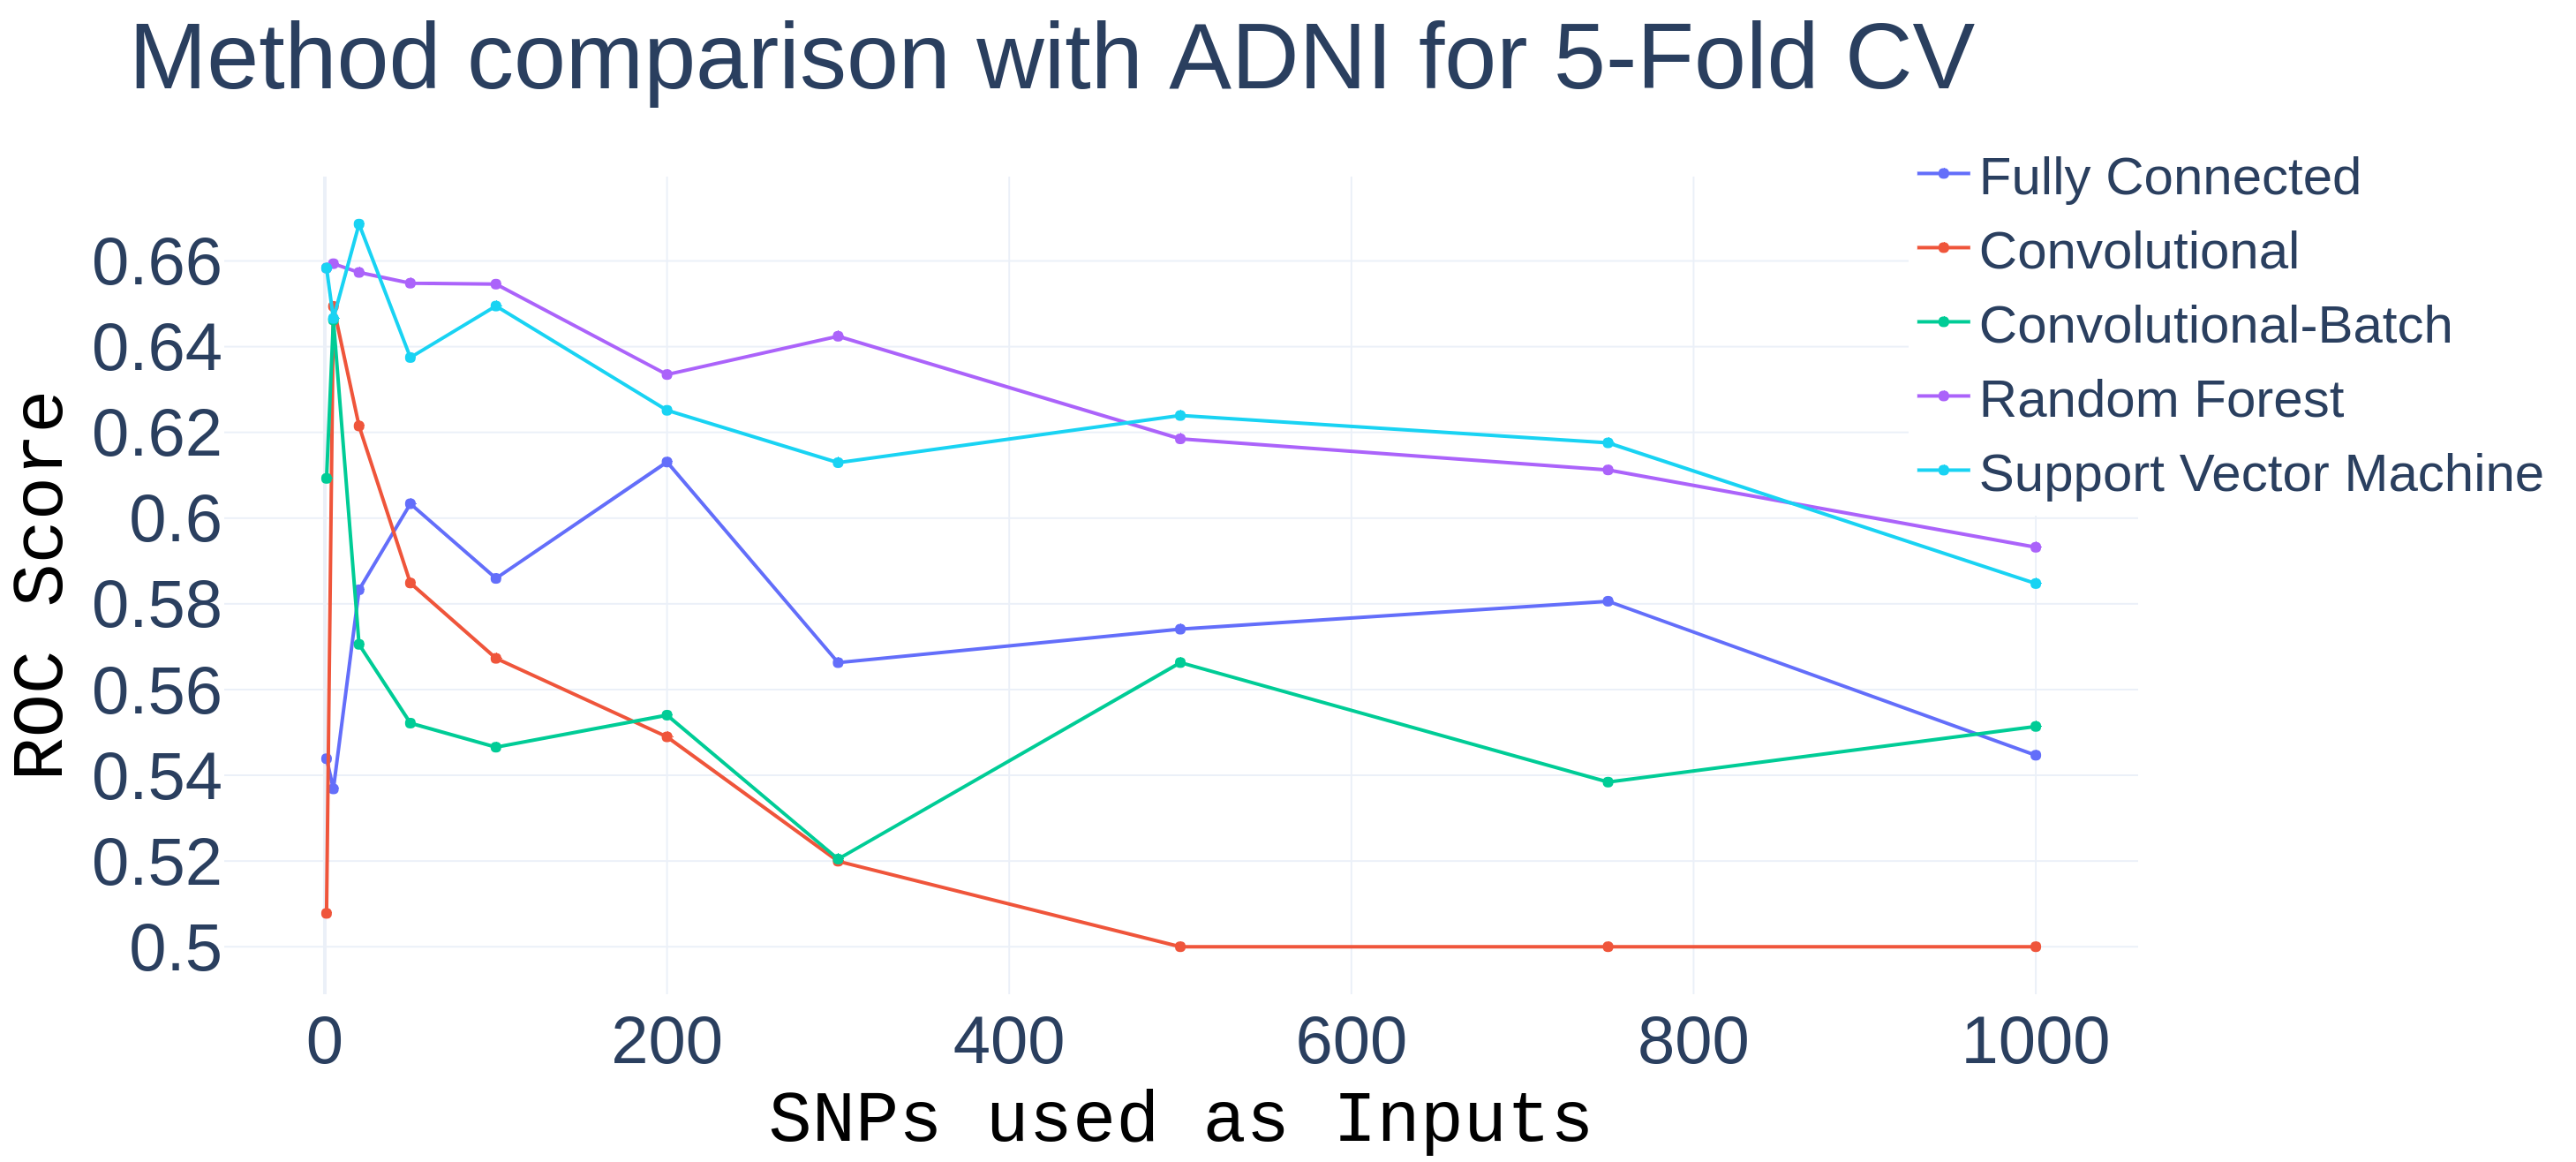
\includegraphics[width=4in]{images/results/AdniCV.png}}
\caption{{\bf Method comparison using the Complete ADNI dataset}
Analysis of the performance in terms of ROC AUC Score of the different classification methods when increasing the number of SNPs used as inputs, using 5-fold CV with the complete ADNI dataset .The SNPs used are in a descending order of statistical importance, with lower p-values as the first SNPs.}
\label{fig4}
\end{figure}

% Place figure captions after the first paragraph in which they are cited.
\begin{figure}[!ht]
\centerline{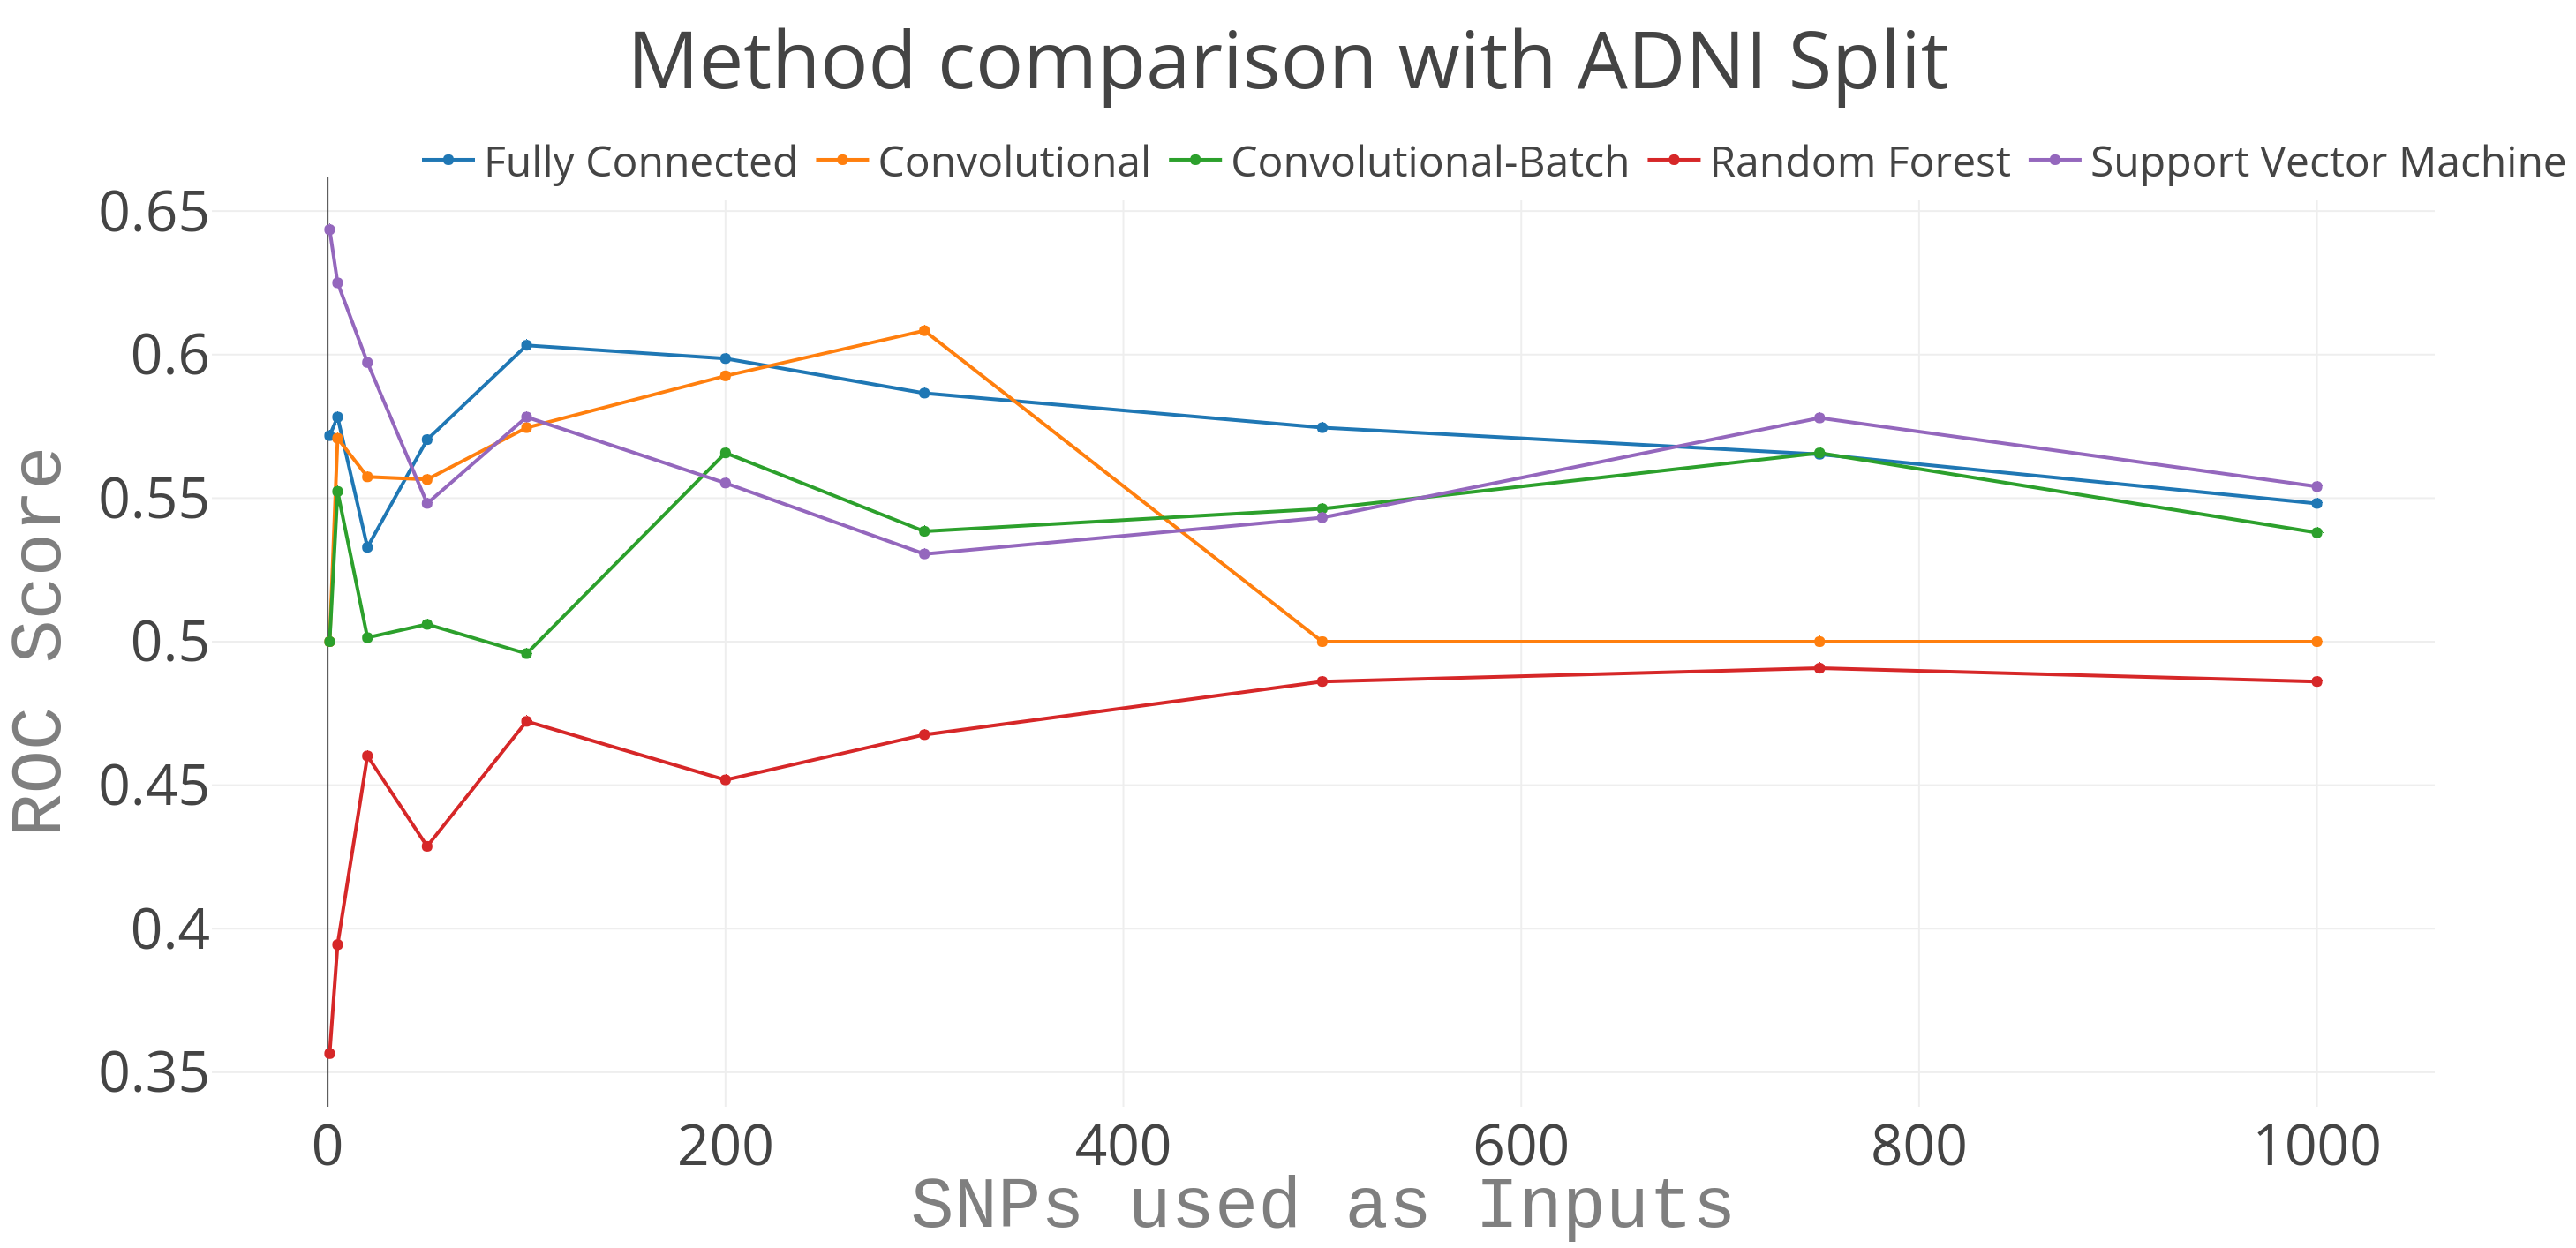
\includegraphics[width=4in]{images/results/AdniSplit2.png}}
\caption{{\bf Method comparison using the Split ADNI dataset}
Analysis of the performance in terms of ROC AUC Score of the different classification methods when increasing the number of SNPs used as inputs, training the model on the ADNI1 and ADNI GO samples and testing it in the IGAP-independent ADNI 2 Samples. }
\label{fig5}
\end{figure}

\section{Simulation}

The next step taken is to attempt to simulate a disease and find out the performance of the methods when utilizing a larger data set. With the simulation it can be clearly seen that the use of a higher number of data samples leads to a much more precise classification as shown in Figure 6. And more interestingly, the increase in the number of samples and makes it so that using a higher number of SNPs as input becomes more valuable. Thus with small data sets it makes sense to use the highest-rated SNPs, but by introducing more SNPs in large data sets the results are refined further and a more precise classification can be achieved. This can be seen in Figures 4.3, and 4.4. For a direct contrast between the performance using two different subsets (500 and 10,000 respectively) Figure 4.5 and 4.6 can be analyzed to see how the performance increase is substantial.


% Place figure captions after the first paragraph in which they are cited.
\begin{figure}[!ht]
\centerline{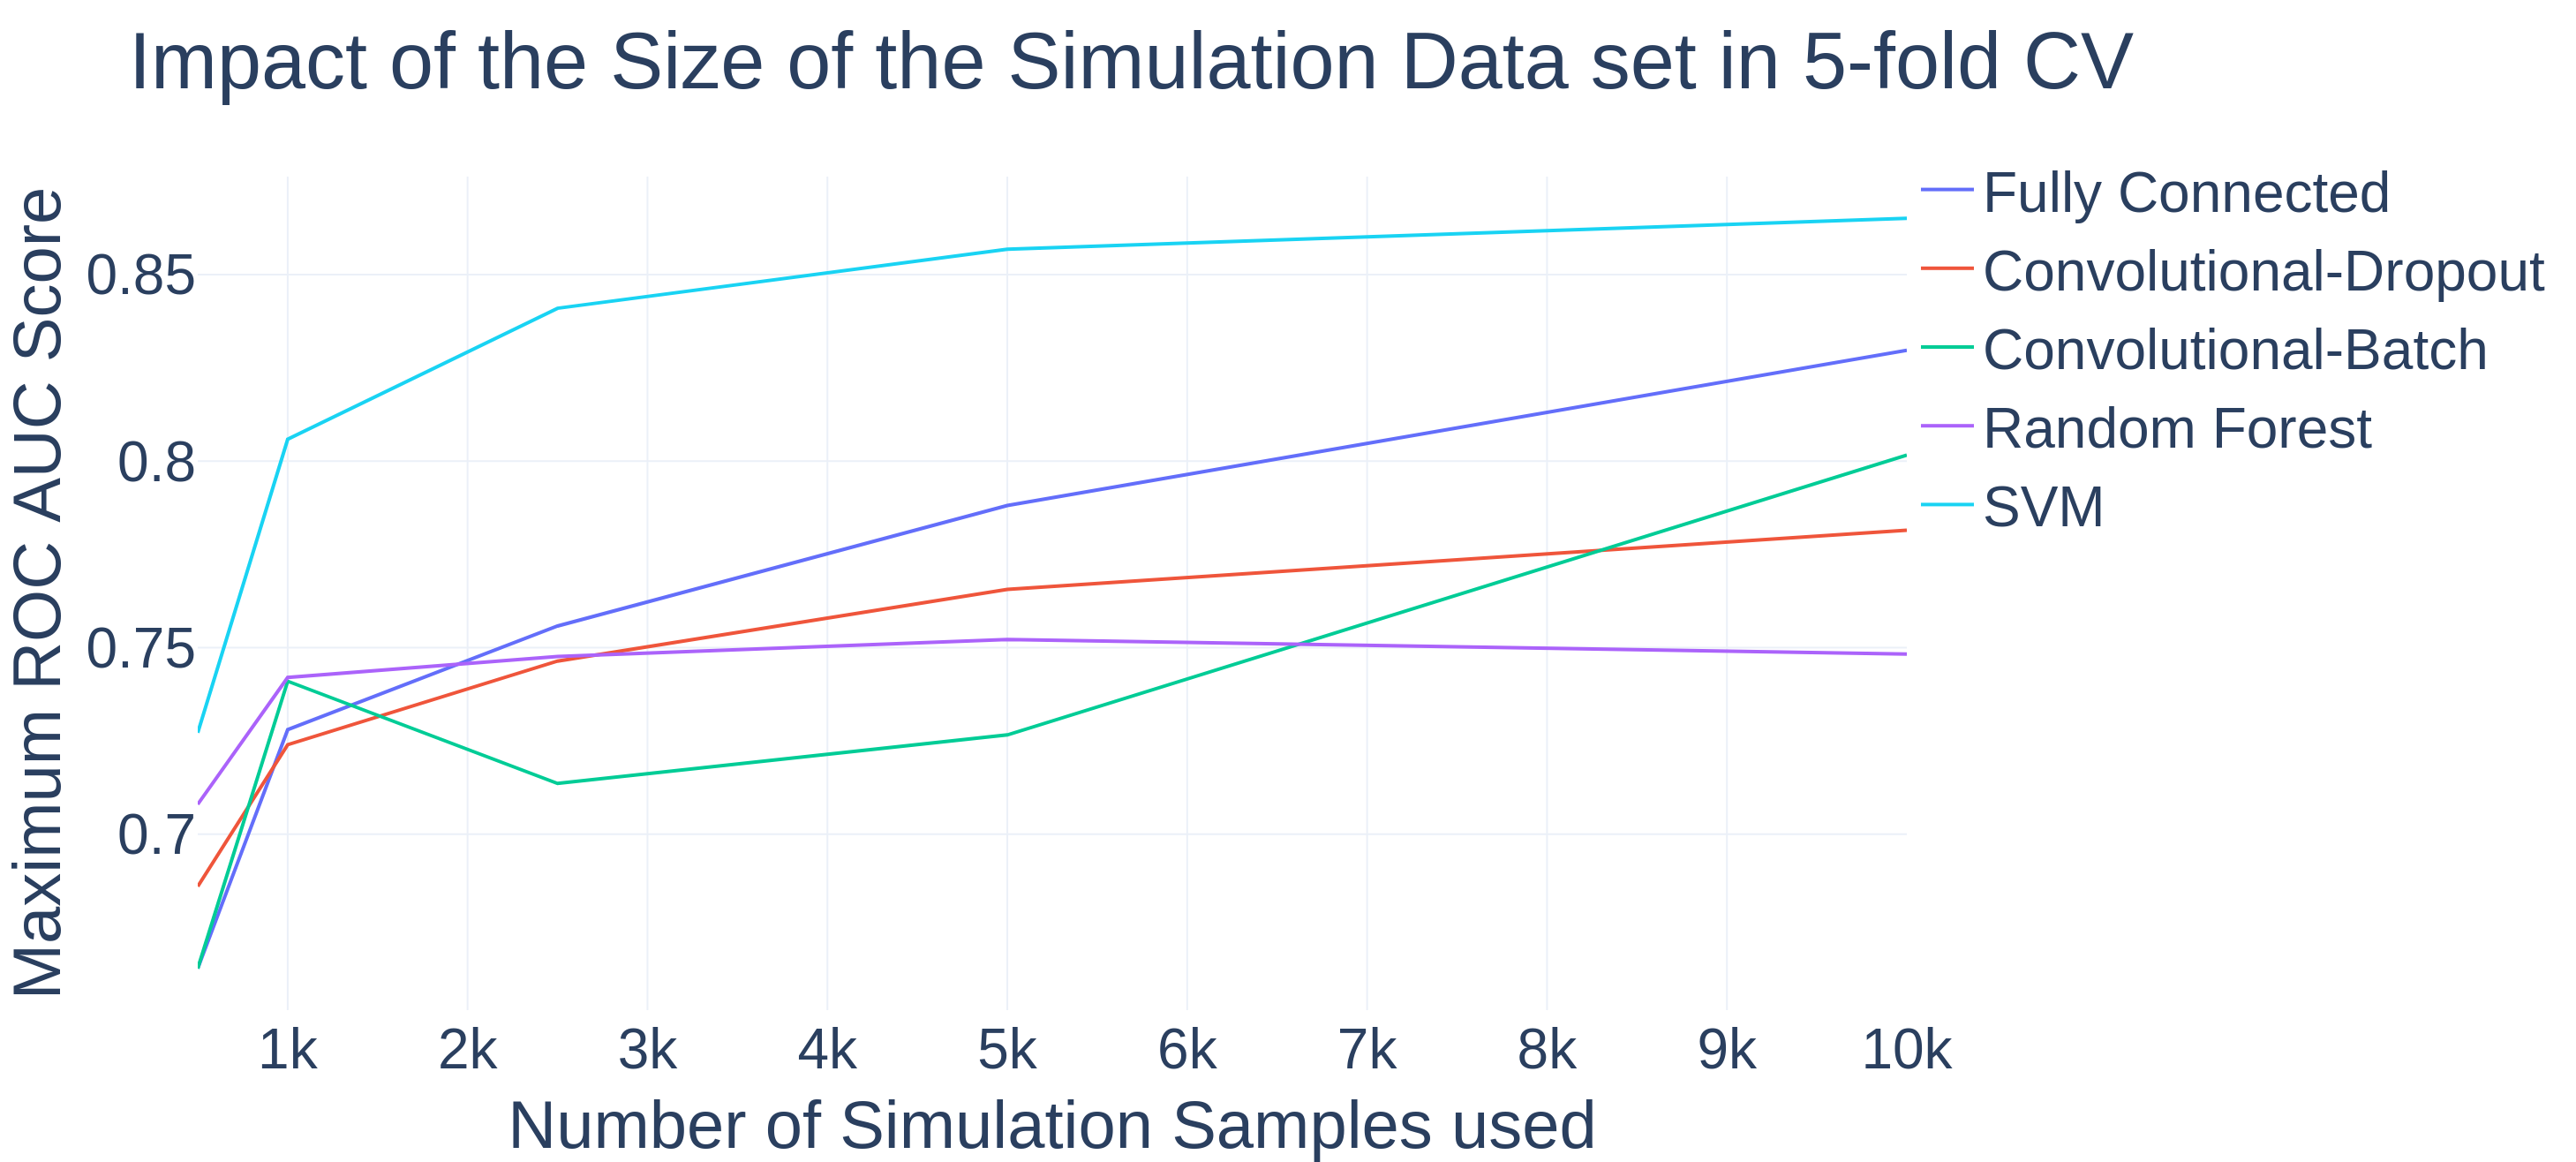
\includegraphics[width=4in]{images/results/ImpactSim.png}}
\caption{{\bf Impact of the subset size on the prediction}
Analysis of the effect in the ROC AUC Score done by increasing the number of samples used for the 5-fold CV in the simulated dataset using the different classification methods.}
\label{fig6}
\end{figure}

\begin{figure}[!ht]
\centerline{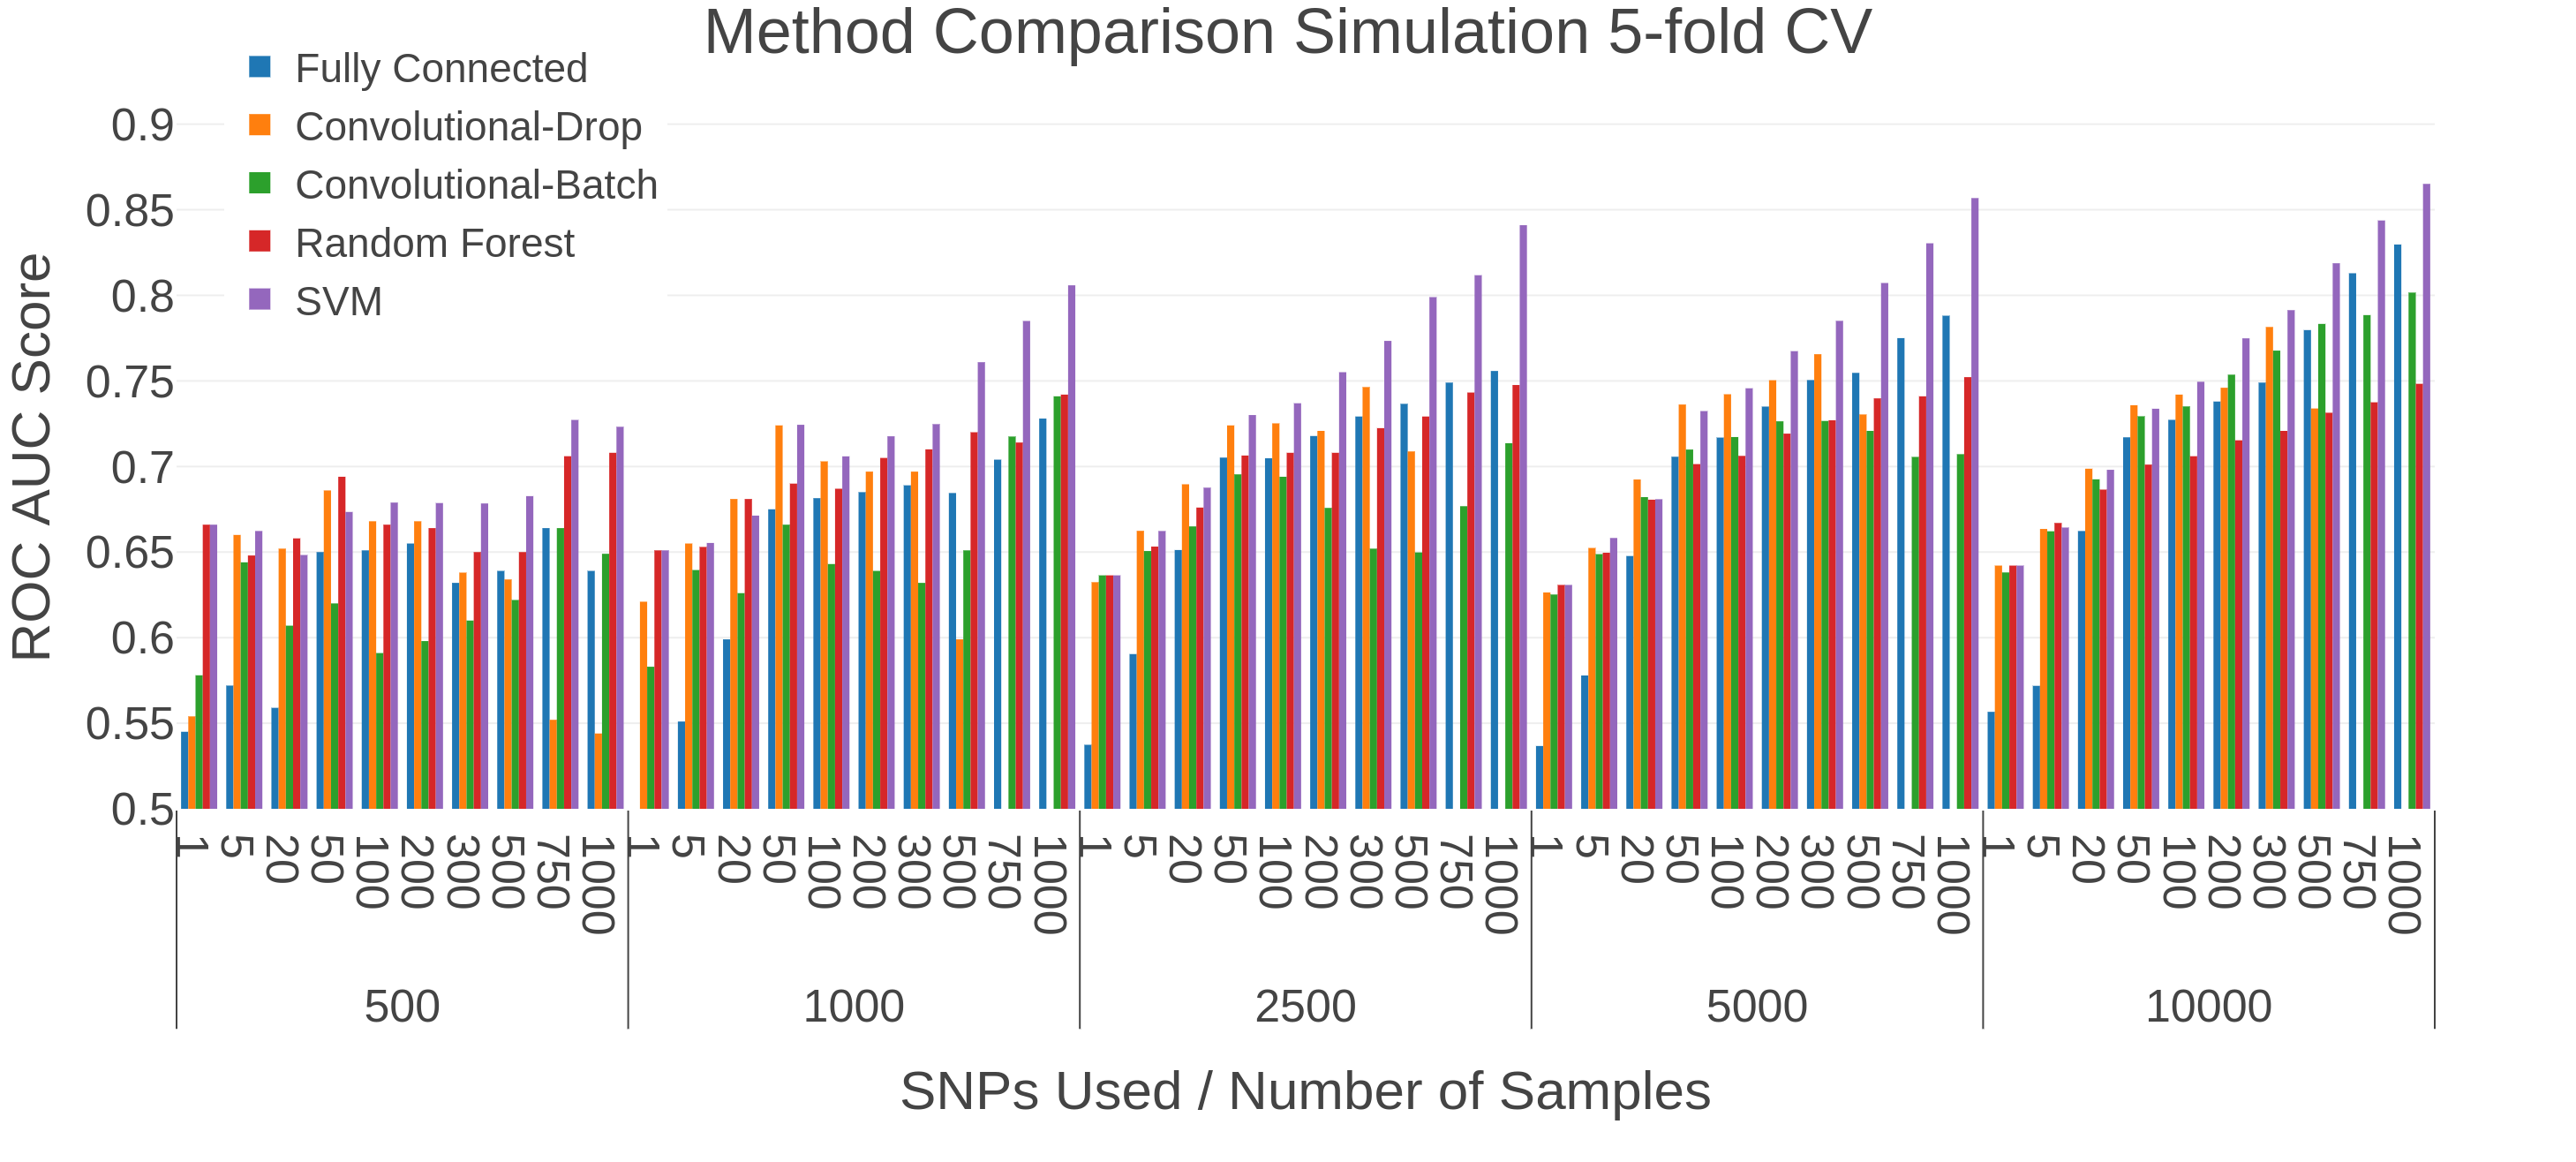
\includegraphics[width=4in]{images/results/SimComplete.png}}
\caption{{\bf Method Comparison with Simulated Dataset}
Comparison between the ROC AUC Score obtained using the different classification methods. The X axis firstly describes an increase of the number of SNPS used for classification, and afterwards an increase in the size of the simulation dataset}
\label{fig7}
\end{figure}


\begin{figure}[!ht]
\centerline{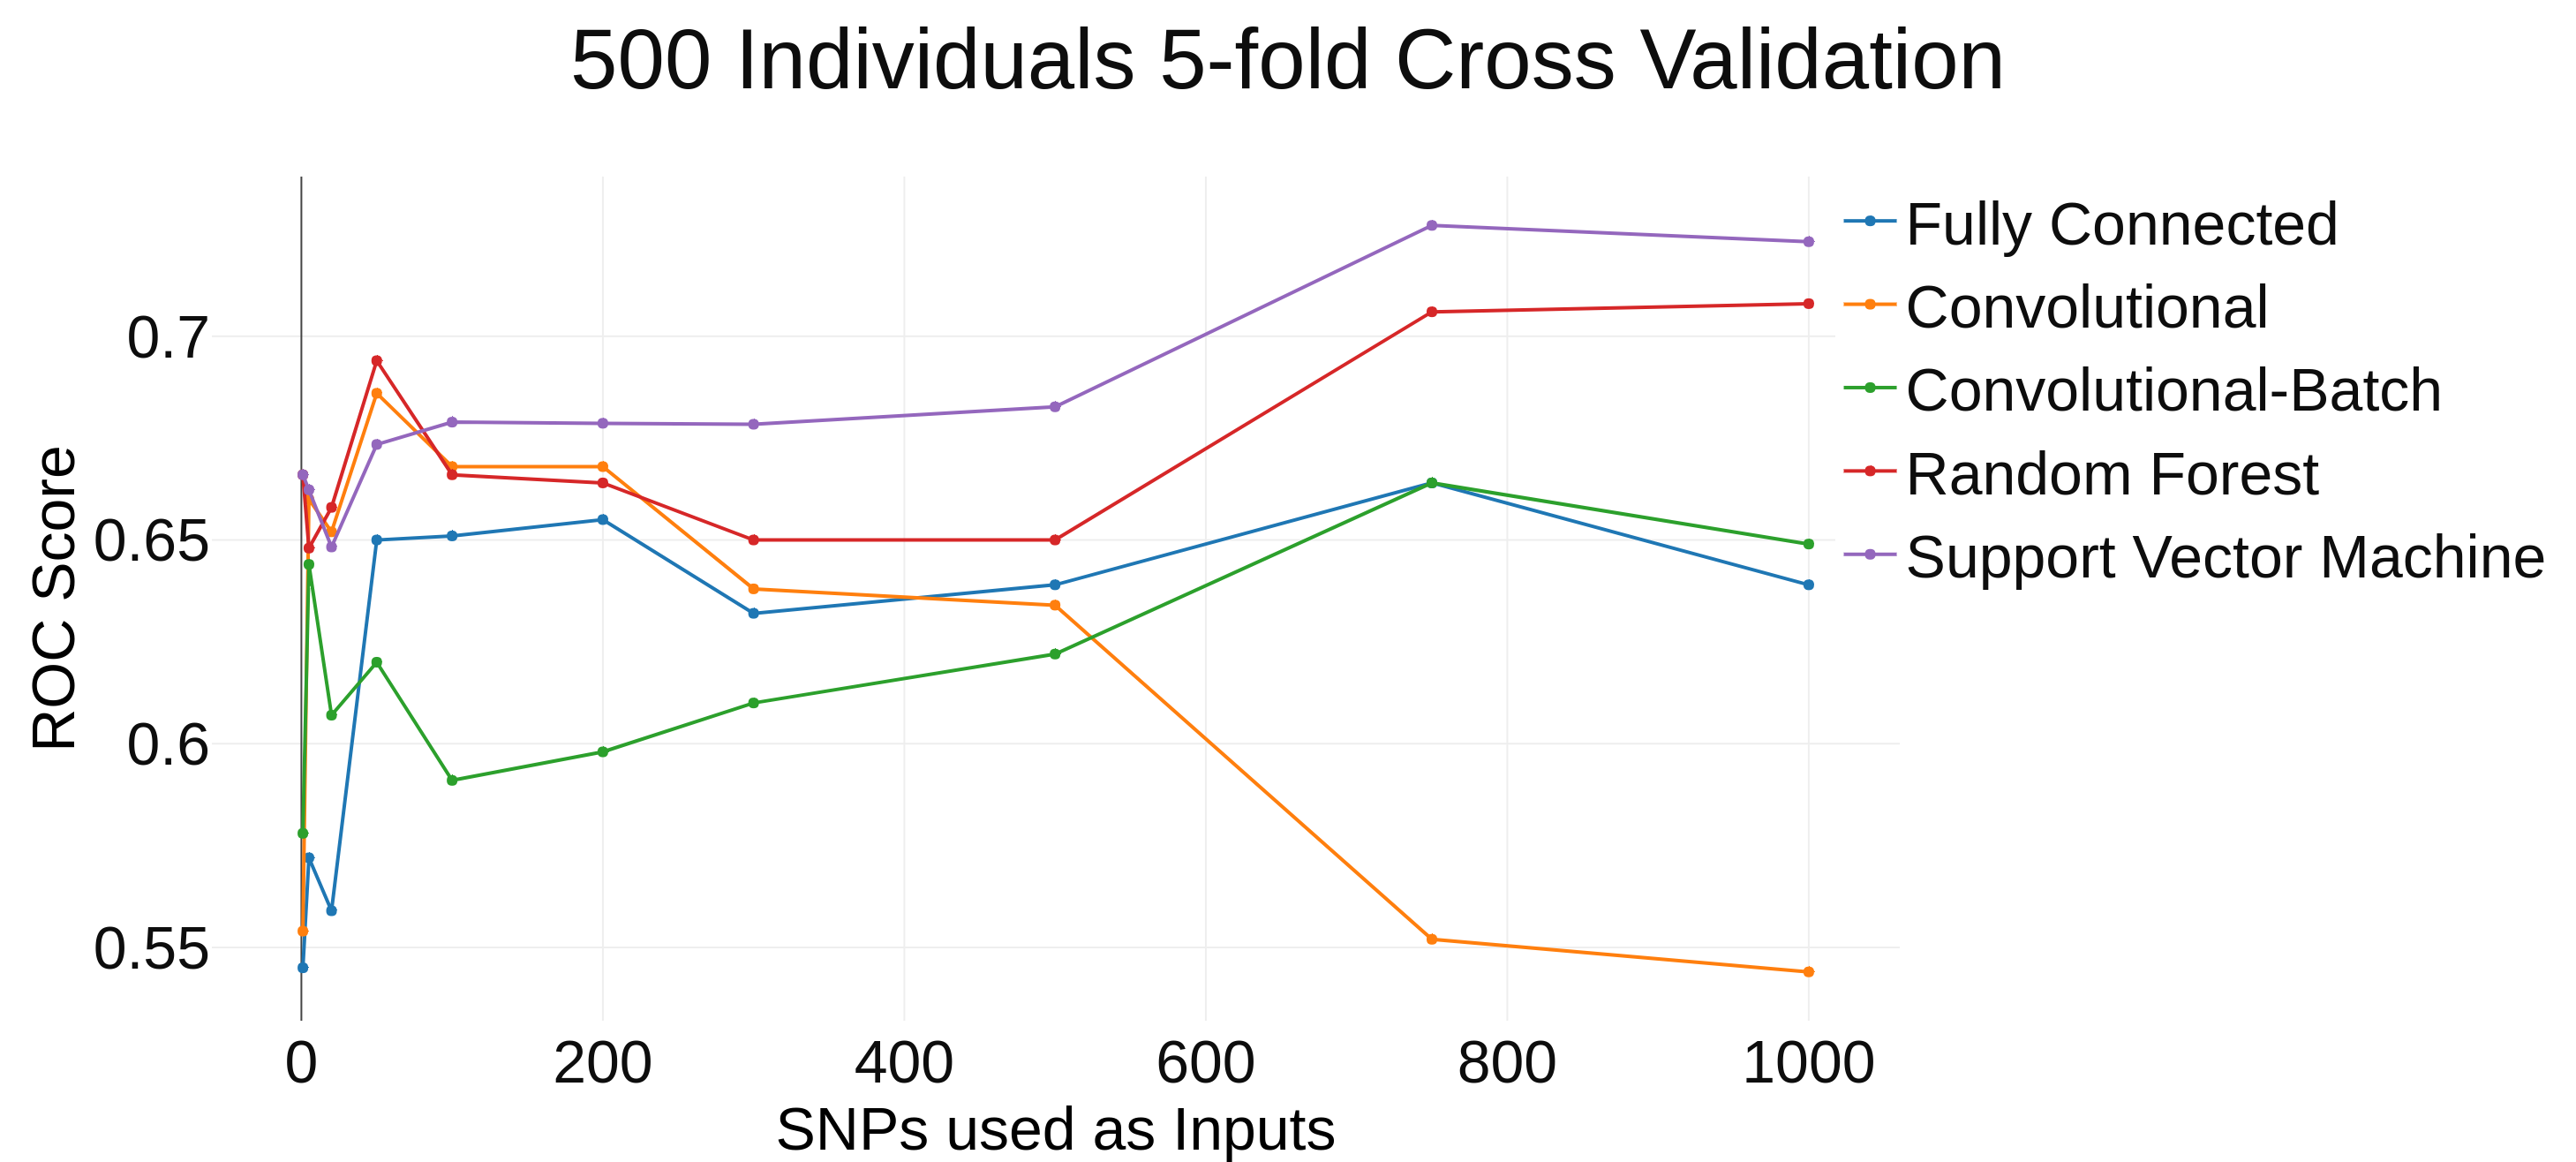
\includegraphics[width=4in]{images/results/Sim500.png}}
\caption{{\bf Method comparison with 500 Individuals}
Comparison of the ROC AUC Score from 5-fold CV using different classification methods while increasing the number of SNPs given a simulation dataset with 500 Individuals}
\label{fig8}
\end{figure}

\begin{figure}[!ht]
\centerline{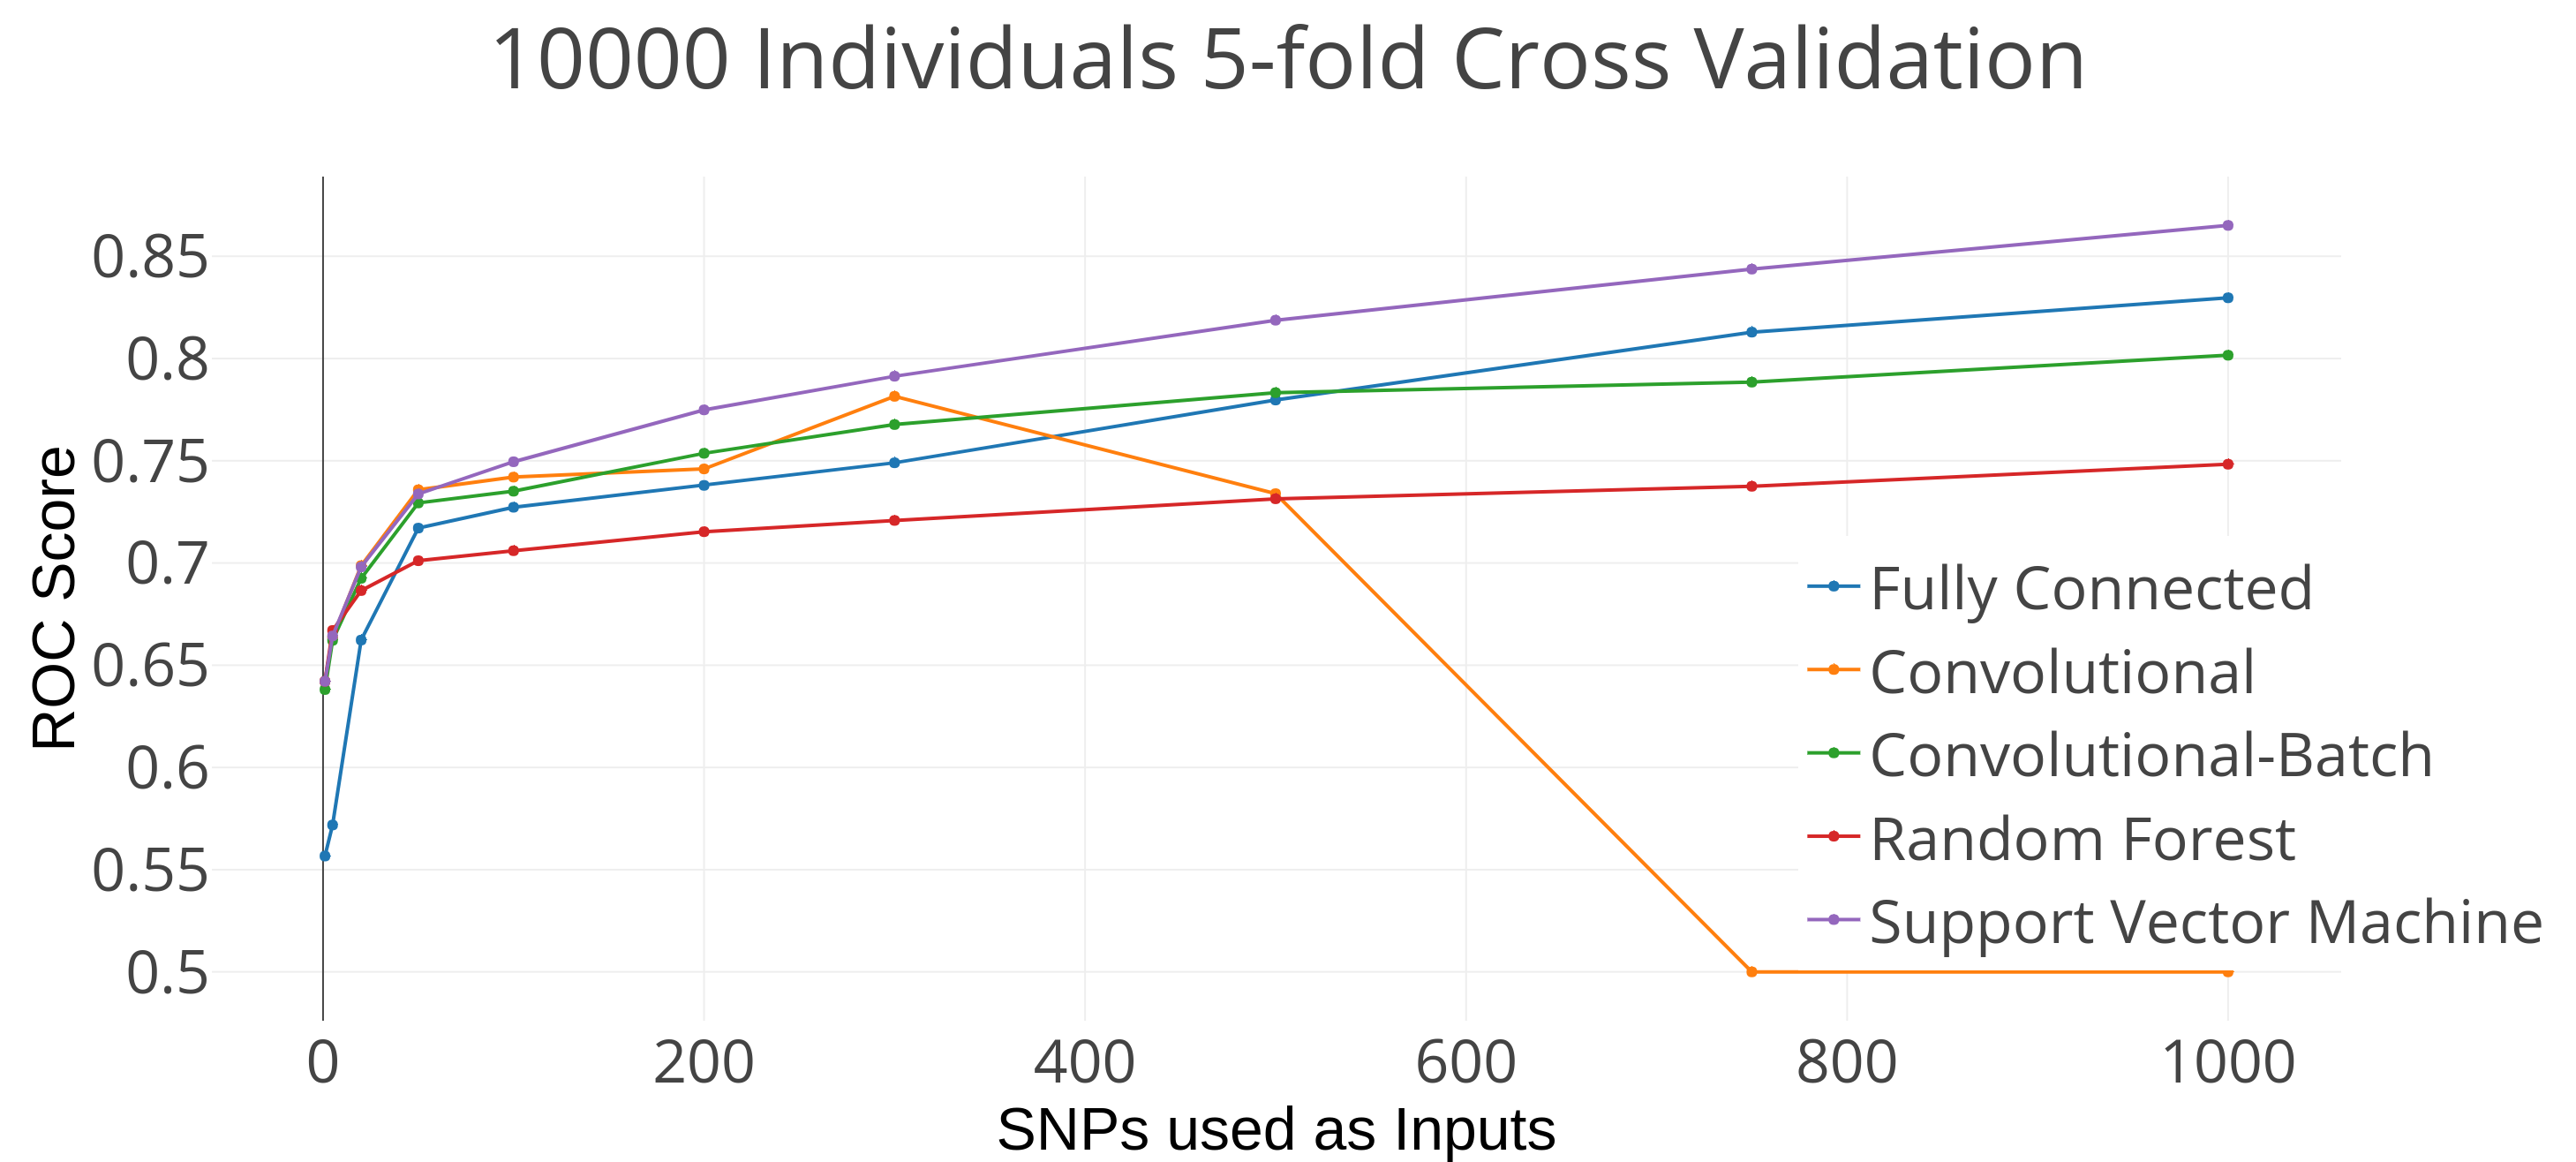
\includegraphics[width=4in]{images/results/Sim10000.png}}
\caption{{\bf Method comparison with 10000 Individuals}
Comparison of the ROC AUC Score from 5-fold CV using different classification methods while increasing the number of SNPs given a simulation dataset with 10,000 Individuals}
\label{fig9}
\end{figure}
\clearpage
\section{Data Augmentation}

The results from the previous simulation show that the use of more samples should benefit the prediction in the Alzheimer's task. Thus,  the artificially augmented data set is generated for training purposes and used the ADNI data set as the test set. In this case the increase in the number of samples did not directly mean a better performance and a higher use of SNPs, as it can be seen, once the system starts using over 100 SNPs the performance on the ADNI subset tends to decay. Plus, the increase in size of the training data set also did not mean constant increases as in the previous scenario. It is shown that the use of more SNPs coupled with a decent size of artificially-augmented samples gives the best results on the ROC Score, which shows that both of these factors have a role to play in the prediction. The convolutional dropout network did have some issues when using too much SNPs and dropped to a classification, and in general the simpler models such as Random Forest and Support Vector Machine performed better. This shows that there is only so much that can be accomplished with data augmentation, and that the disease might actually be focused on a smaller number of uncorrelated genes as supposed in the simulation. Figures 4.7 and 4.8 illustrate these results.

% Place figure captions after the first paragraph in which they are cited.
\begin{figure}[!ht]
\centerline{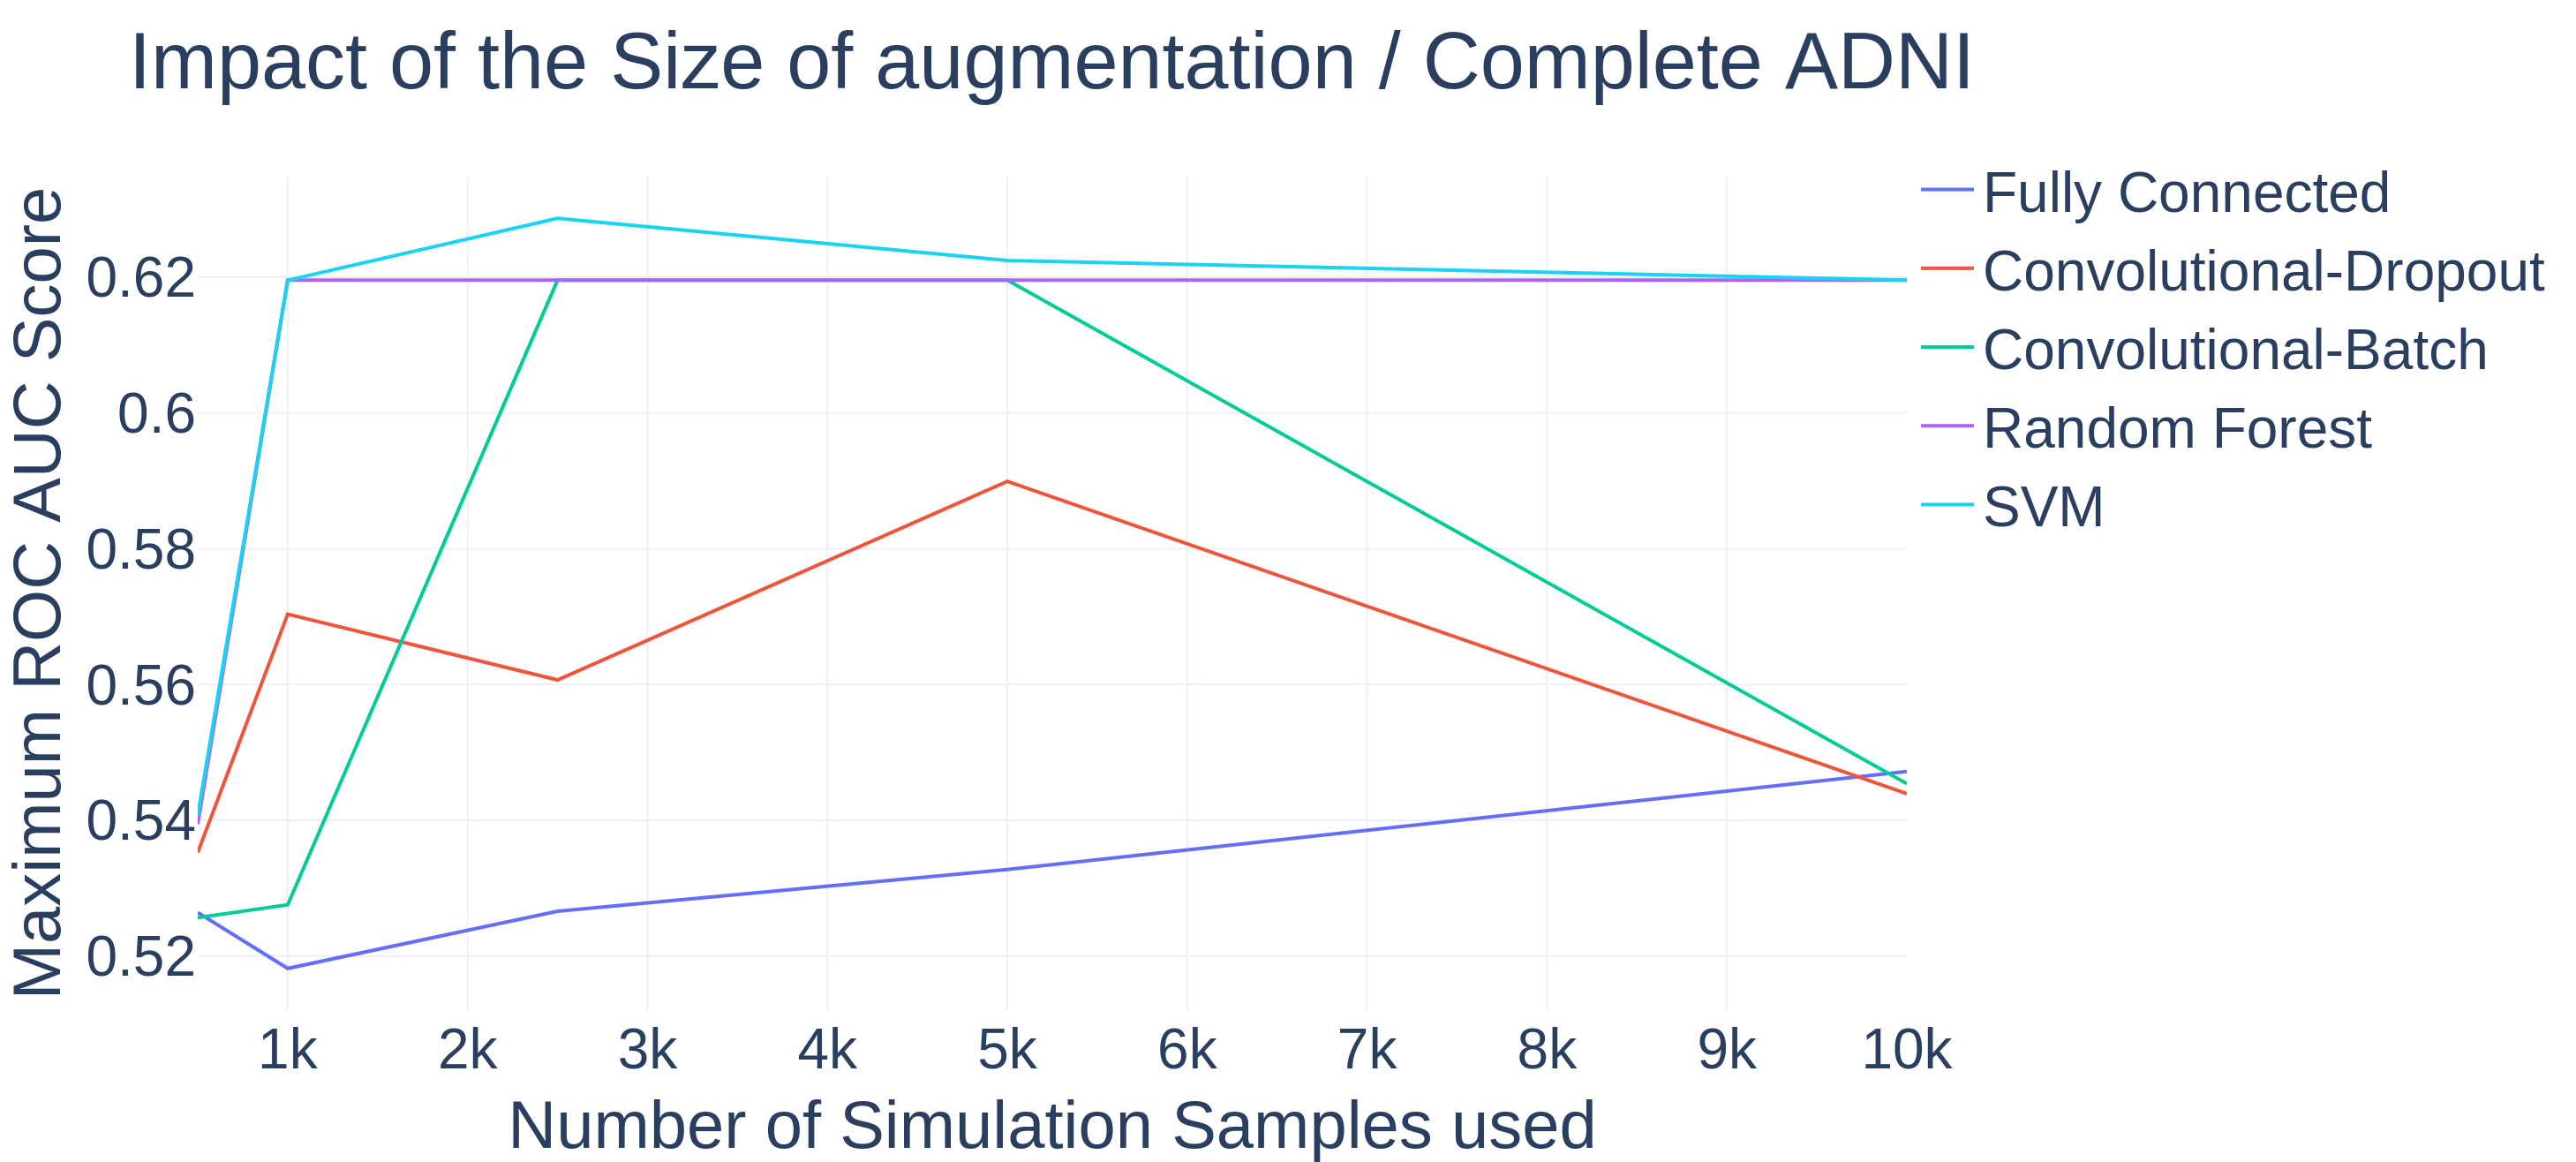
\includegraphics[width=4in]{images/results/ImpactDataAug.png}}
\caption{{\bf Impact of the augmentation size on the prediction}
Analysis of the effect in the ROC AUC Score done by increasing the number of data-augmentation samples used for the training segment validated on the complete ADNI Dataset using the different classification methods.}
\label{fig10}
\end{figure}

\begin{figure}[!ht]
\centerline{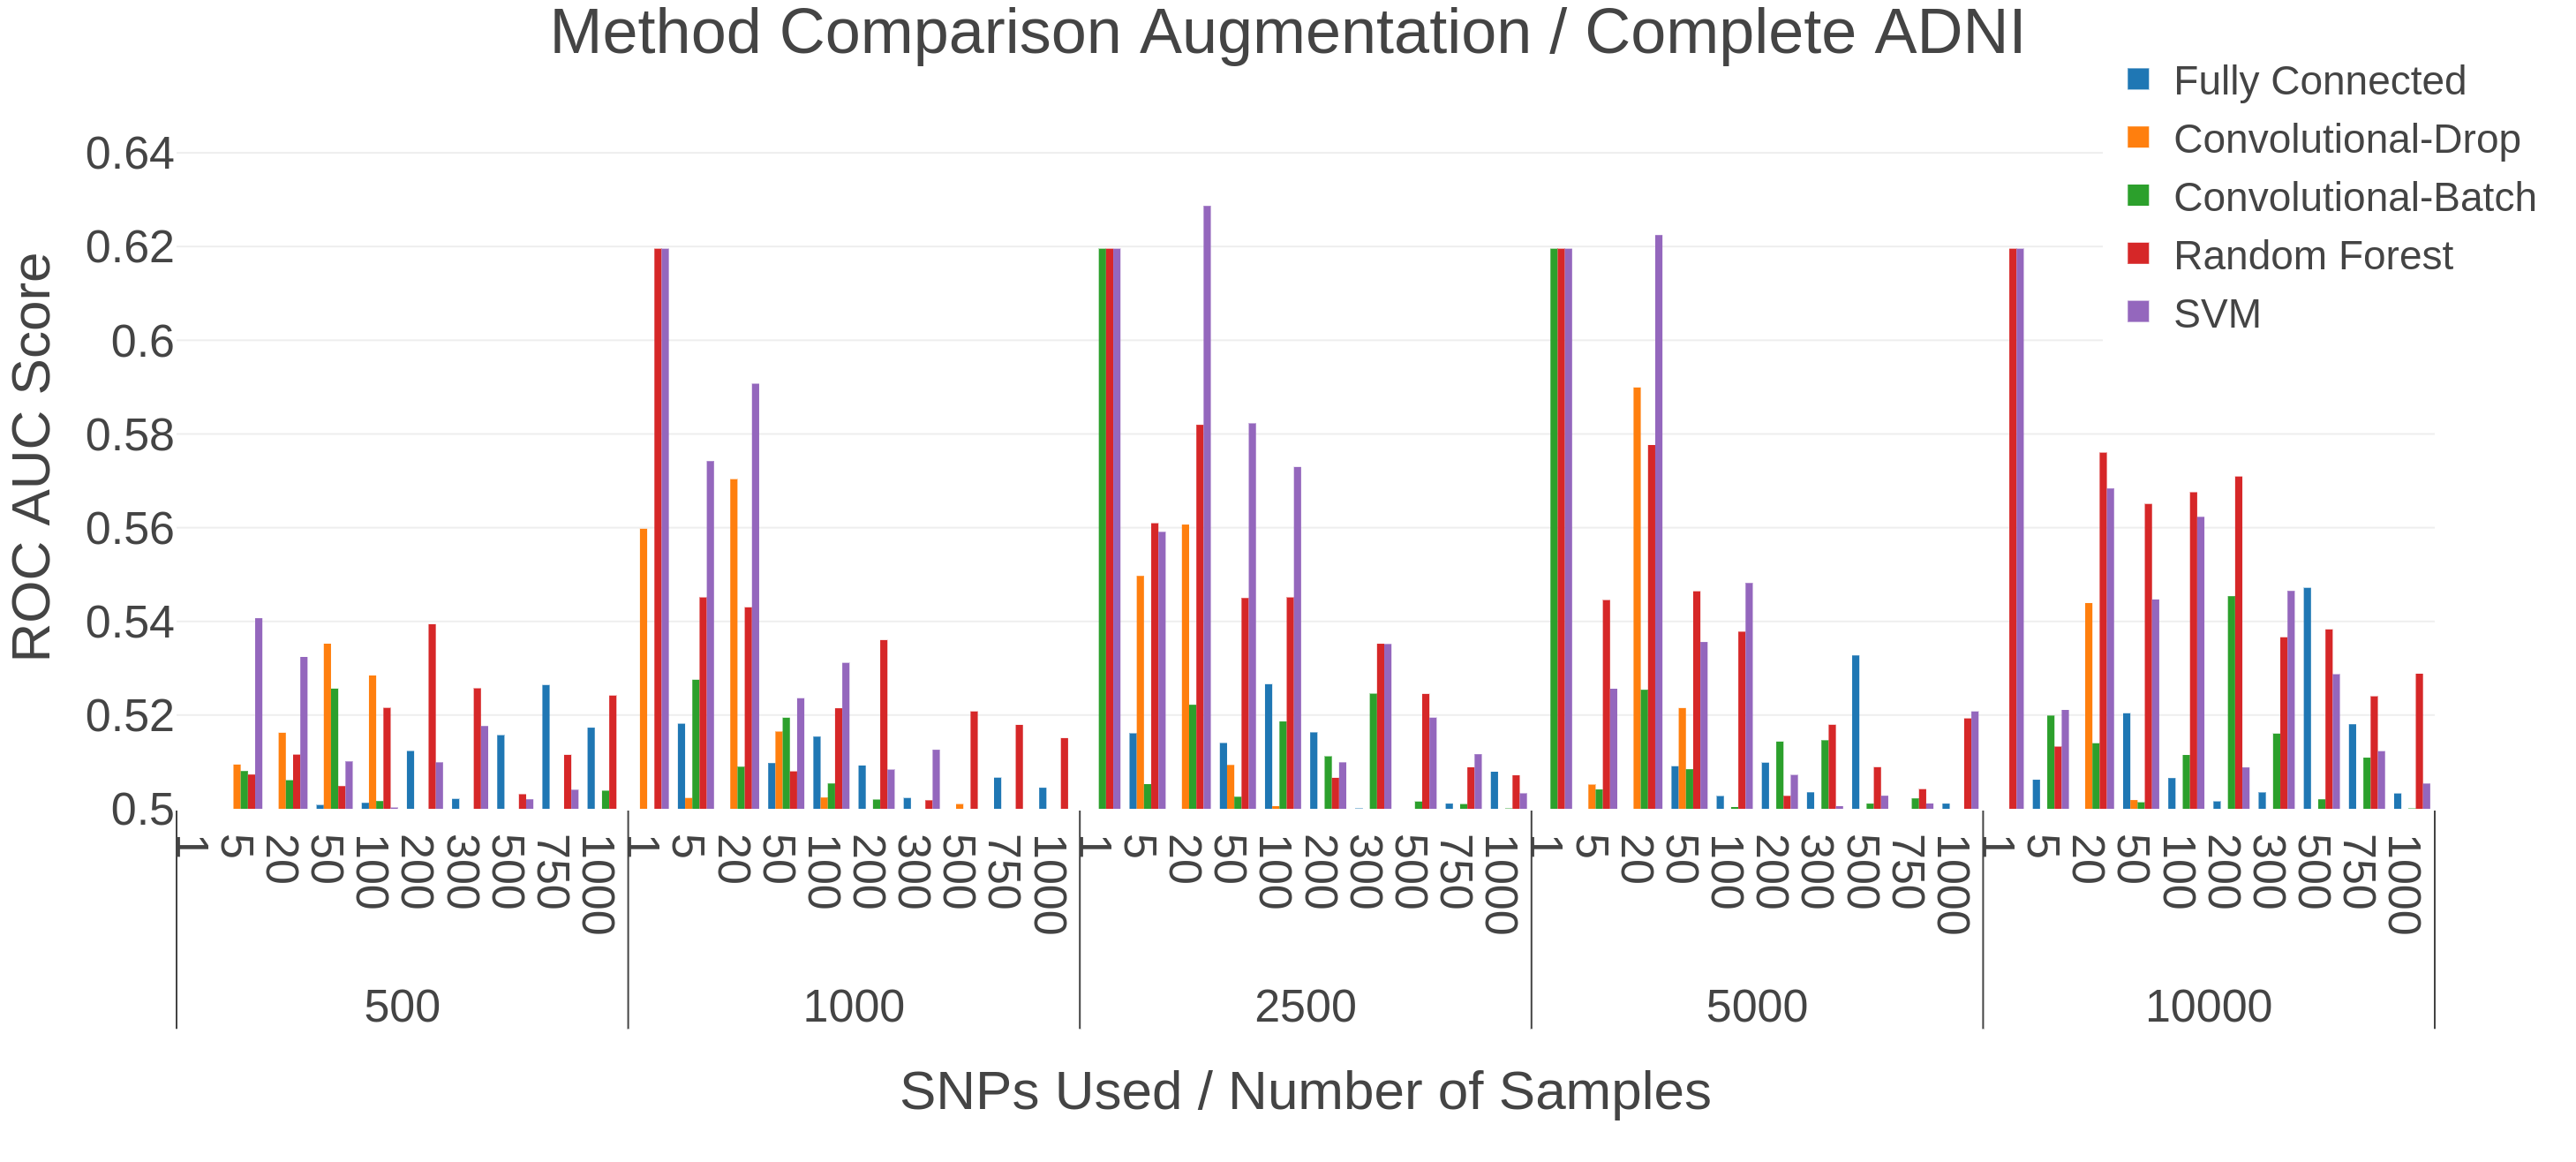
\includegraphics[width=4in]{images/results/DataAugComplete.png}}
\caption{{\bf Method Comparison with full ADNI Dataset} 
Comparison between the ROC AUC Score obtained using the different classification methods. The X axis firstly describes an increase of the number of SNPs used for classification, and afterwards an increase in the data-augmentation size validated on the complete ADNI dataset}
\label{fig11}
\end{figure}


Further restrictions are imposed on the data set used for testing, as some of the ADNI samples are also taken into account for the IGAP study. Thus the testing is restricted to those individuals who did not participate in the IGAP study. For this case it is shown in Figures 4.9 and 4.10 that due to the small sample size and the class imbalance the results are lower as the previous data set. Specifically they tend to show good results using few amounts of SNPs (APOE $\epsilon4$ mainly) and the increase in sample size used to train does not represent an increase in the prediction capability. This gives us the impression that the learning models either do not generalize correctly, or the few individuals from the unbalanced data set do not correspond to the genetic markers learned from the IGAP-based simulation. Comparing these results with the ones obtained from the ADNI split the results are in average better for the data augmentation process than from the standard. 

\begin{figure}[!ht]
\centerline{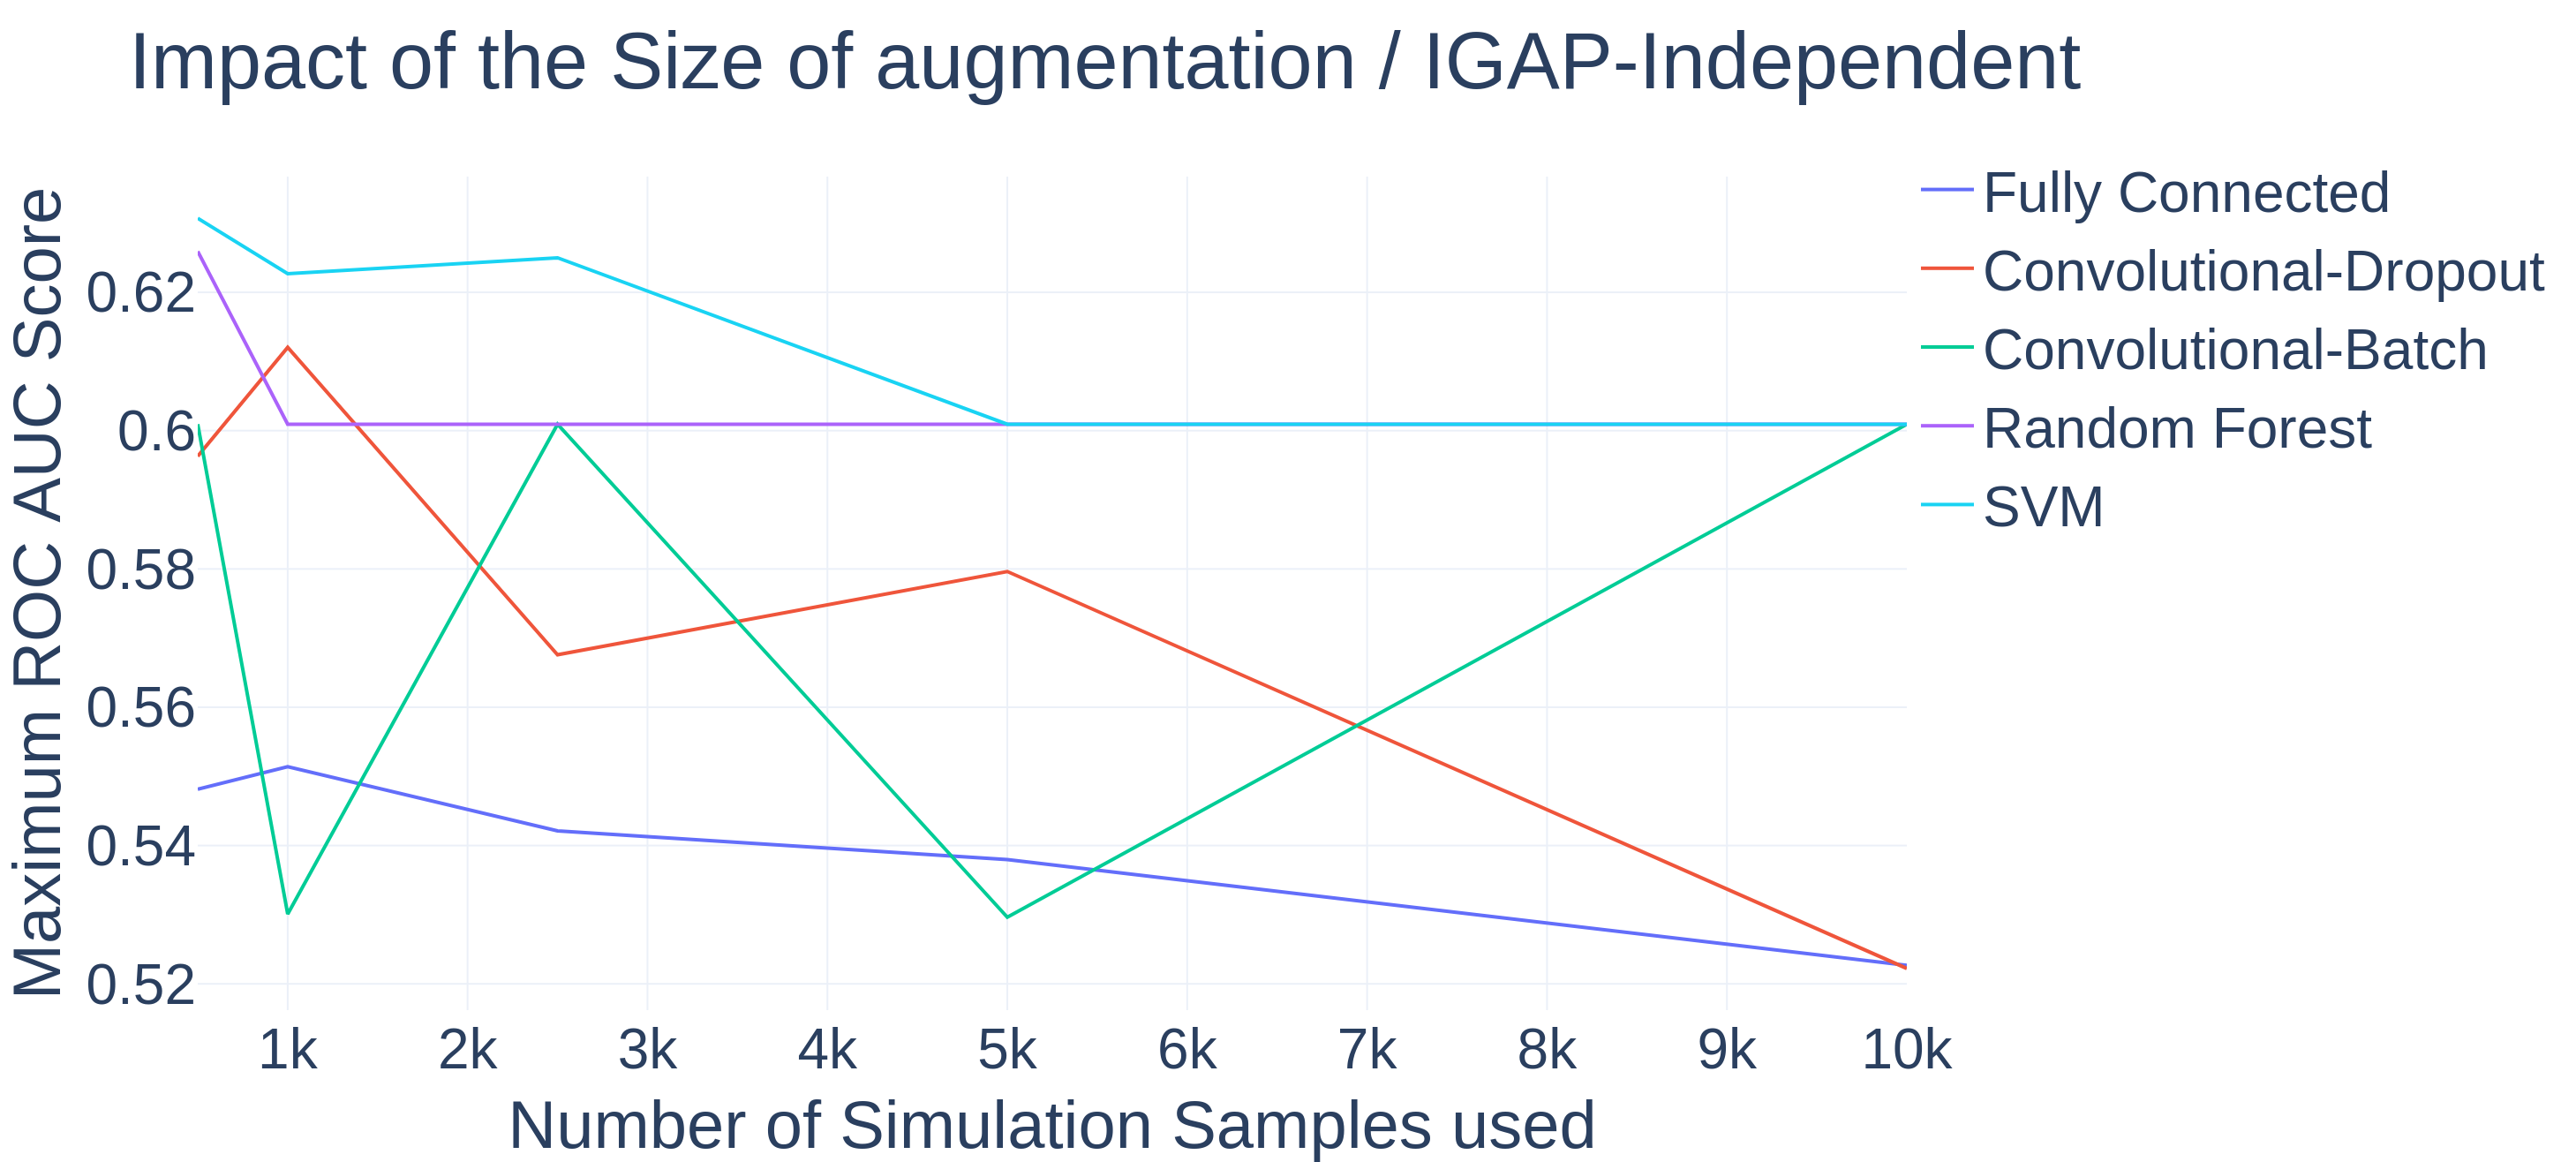
\includegraphics[width=4in]{images/results/ImpactDataAug2.png}}
\caption{{\bf Impact of the augmentation size in IGAP-Independent Subset}
Analysis of the effect in the ROC AUC Score done by increasing the number of data-augmentation samples used for the training segment validated on the IGAP-Independent subset using the different classification methods.}
\label{fig12}
\end{figure}

\begin{figure}[!ht]
\centerline{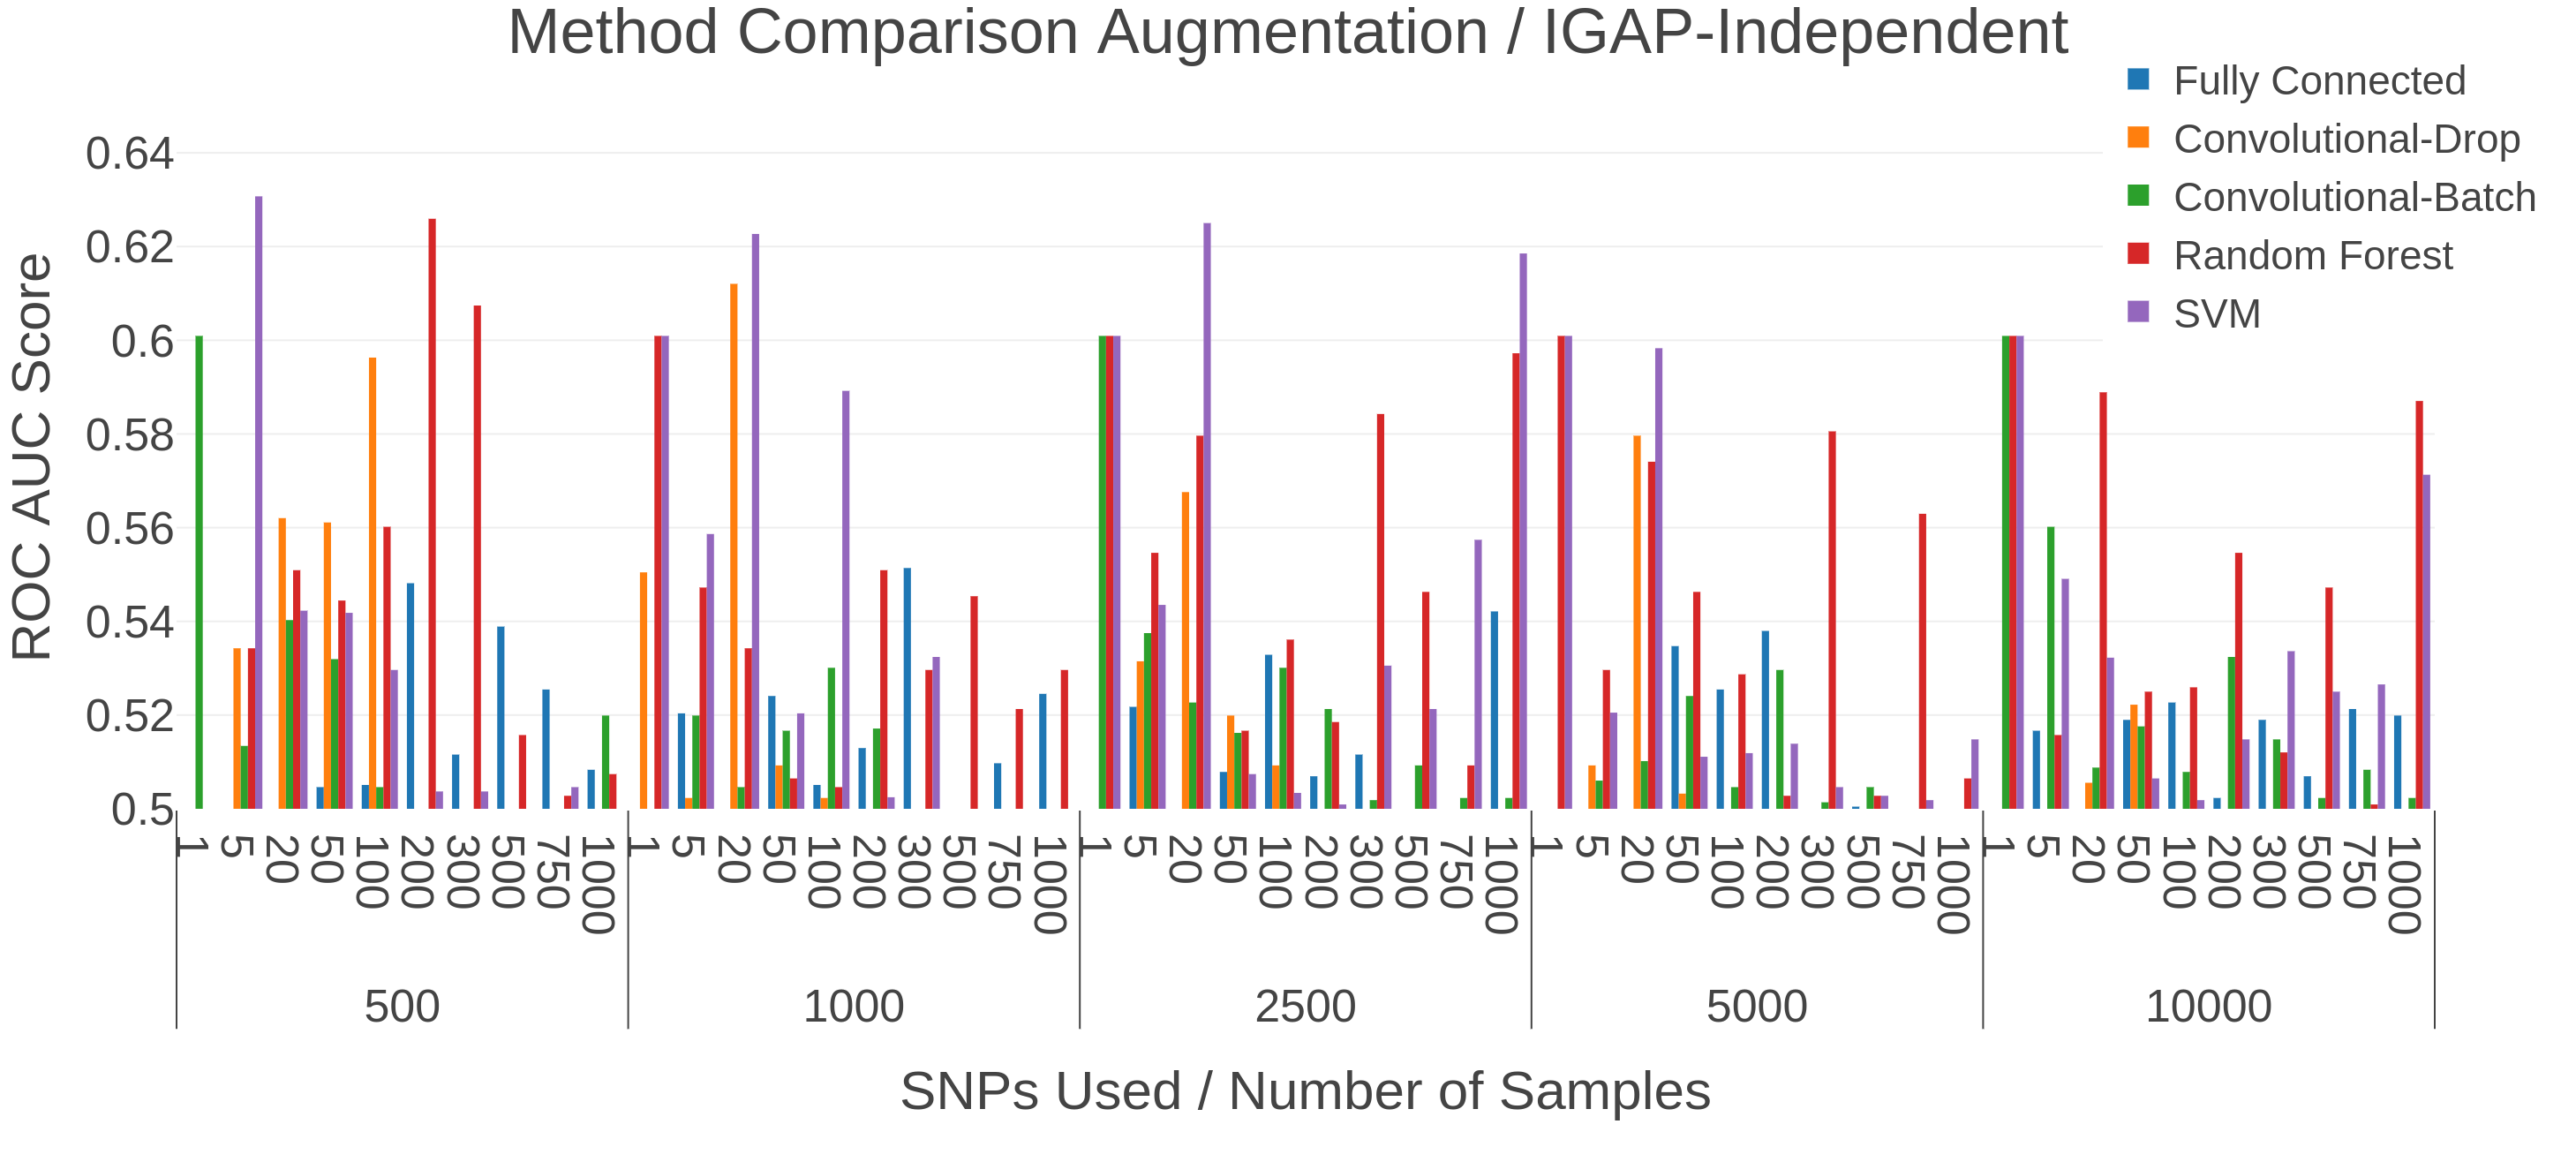
\includegraphics[width=4in]{images/results/DataAugComplete2.png}}
\caption{{\bf Method Comparison with IGAP-Independent Subset}
Comparison between the ROC AUC Score obtained using the different classification methods. The X axis firstly describes an increase of the number of SNPS used for classification, and afterwards an increase in the data-augmentation size validated on the IGAP-Independent subset.}
\label{fig13}
\end{figure}
\newpage
\section{FRESA.CAD}


The first analysis to perform is on the full ADNI dataset using the top 2,500 SNPs. As before, this comes with a caveat, as the full ADNI dataset does include some samples which were present in the IGAP and as such are not completely independent. The results begin by seeing the ROC AUC Score obtained by the different classifiers. Figure 4.11 and 4.12 show this, where it can be seen that the algorithms perform in the order of 0.60\~0.70. BSIWMS, LASSO and RPART show the best results in this case, and definitely the ensemble of the methods is the one with the best performance, achieving a ROC score of 0.719. Thus it can be seen how the use of the ensemble of methods appears to give the best results for the full dataset case, and they appear to outdo the previous methods. 

 \begin{figure}[!ht]
\centerline{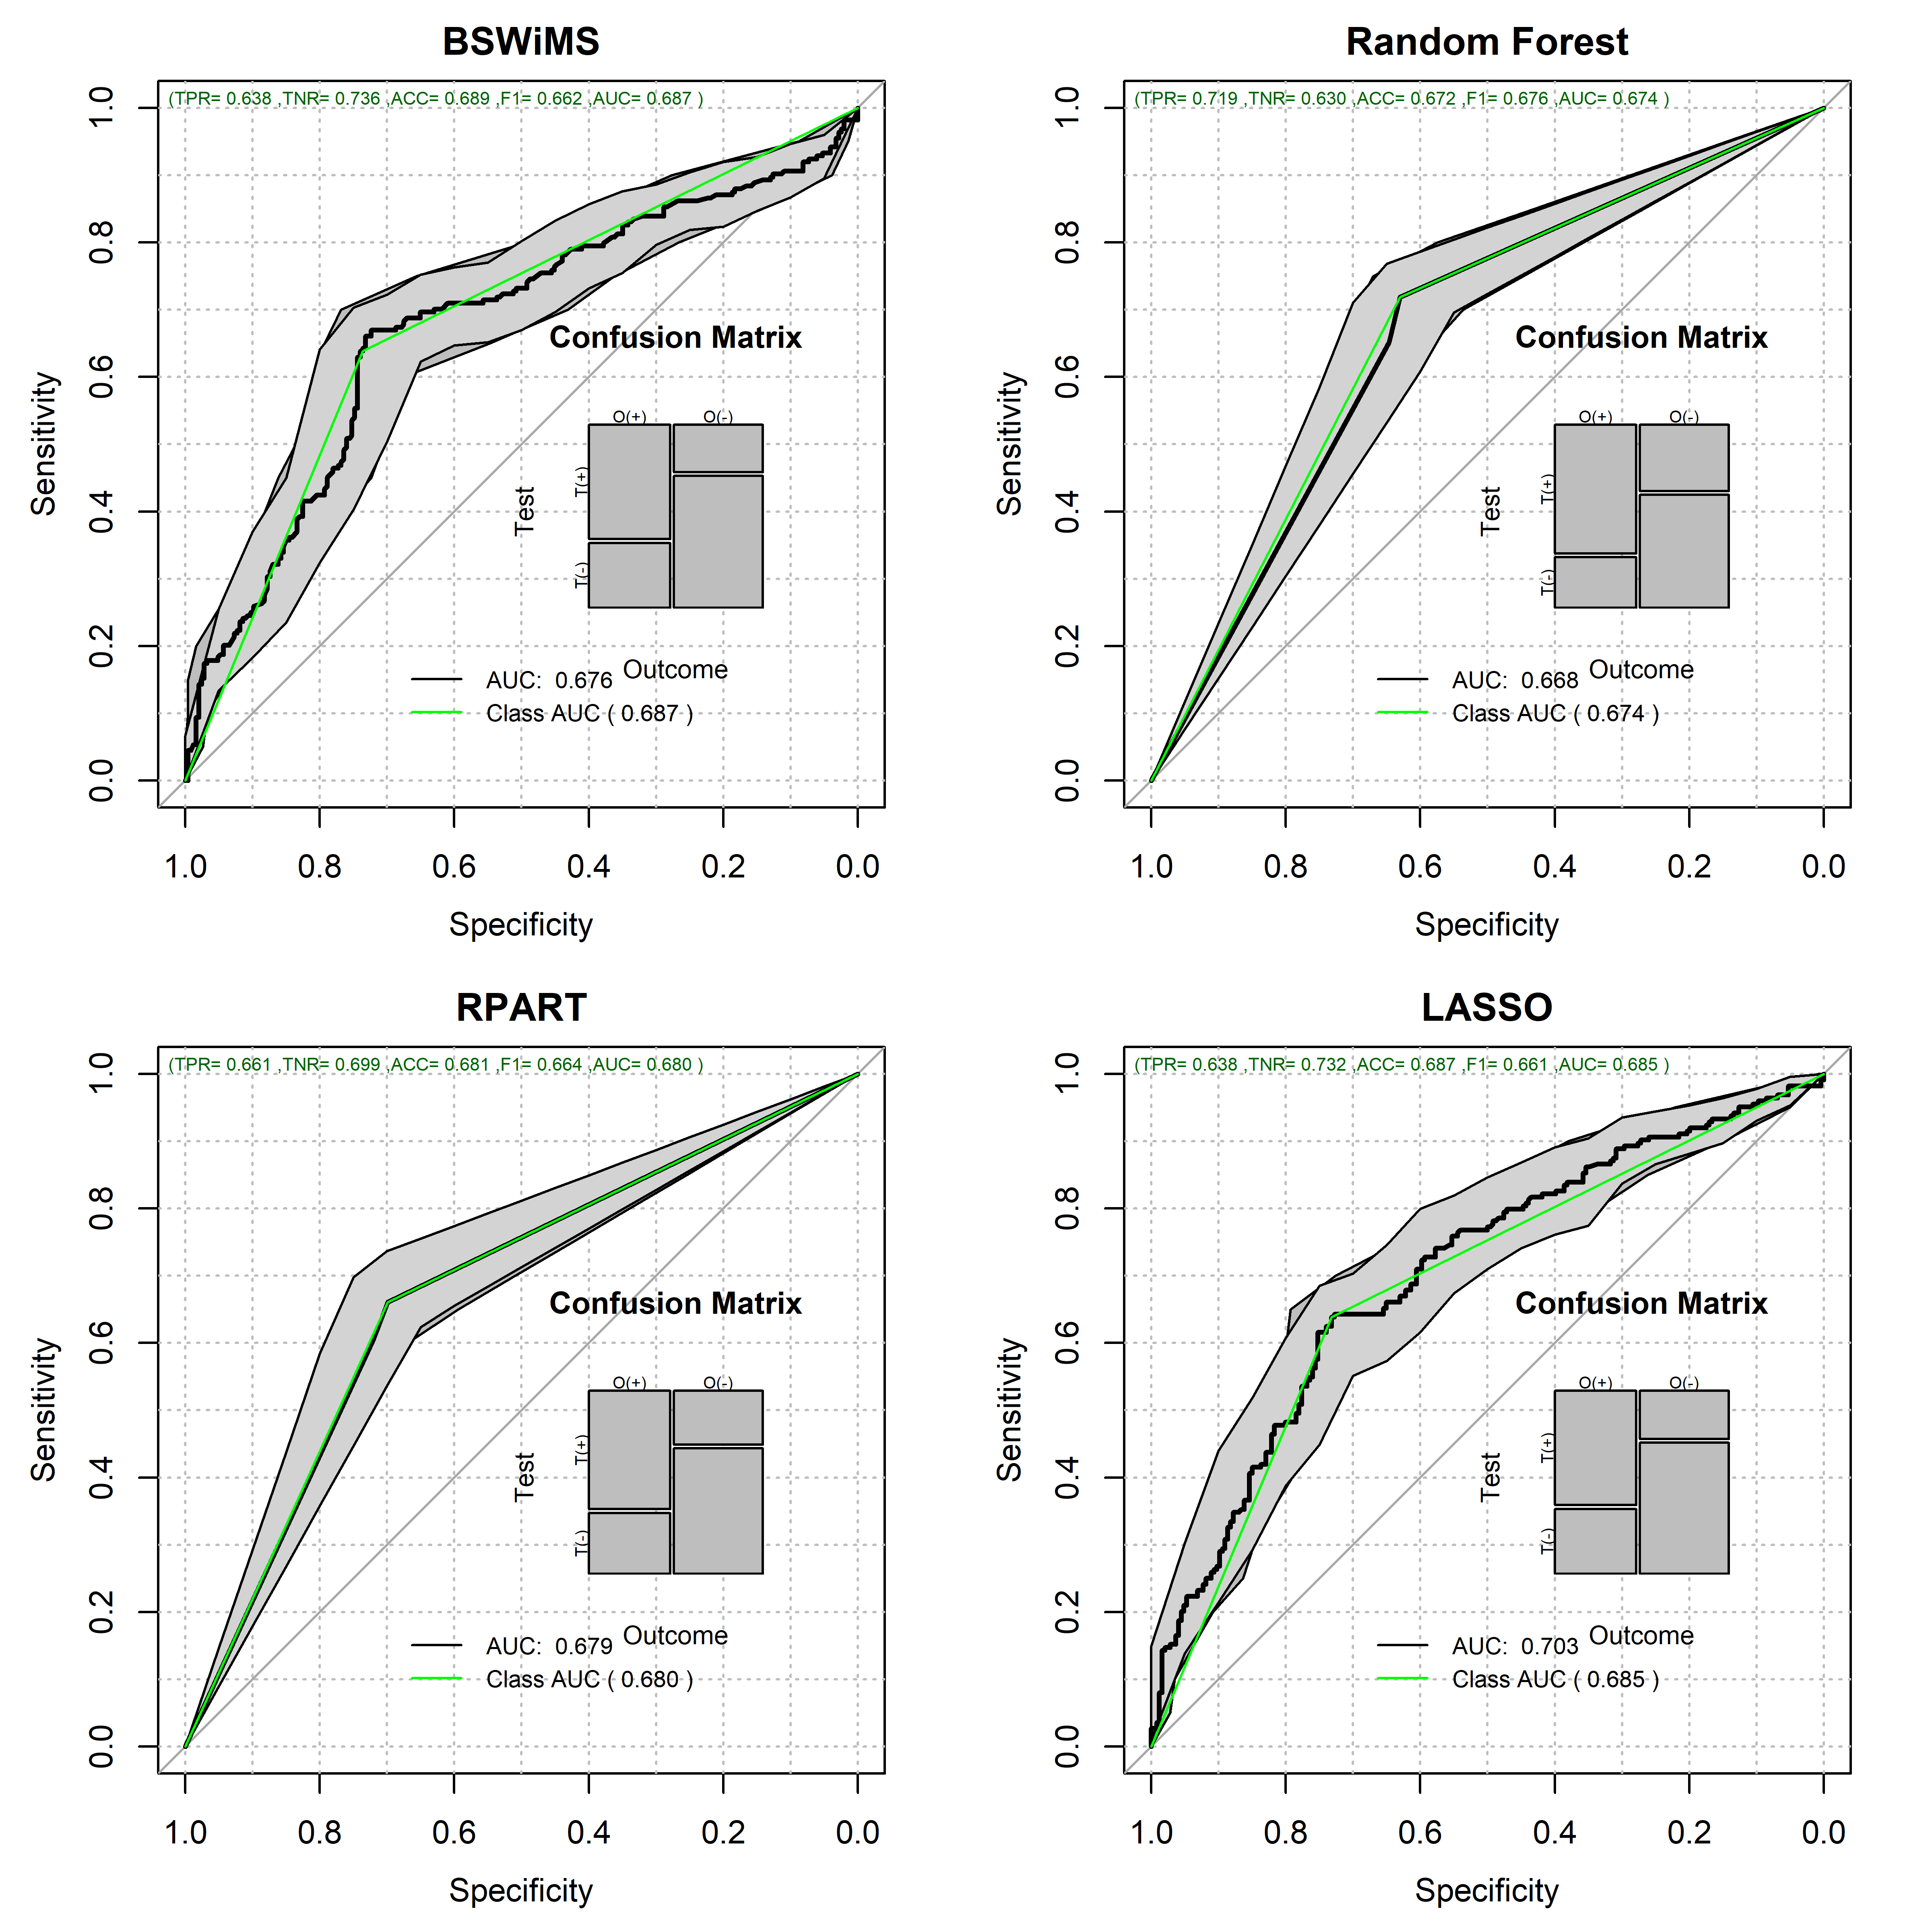
\includegraphics[width=3in]{images/results/fresaCurves1.png}}
\caption{{\bf ROC Curves for the FRESA.CAD Benchmarking Classifiers} 
ROC Curves obtained using BSWiMS, Random Forest, RPART and LASSO of the FRESA.CAD Benchmarking with the complete ADNI dataset for the Cross-Validation and the top 2,500 SNPs as inputs}
\label{fig14}
\end{figure}

 \begin{figure}[!ht]
\centerline{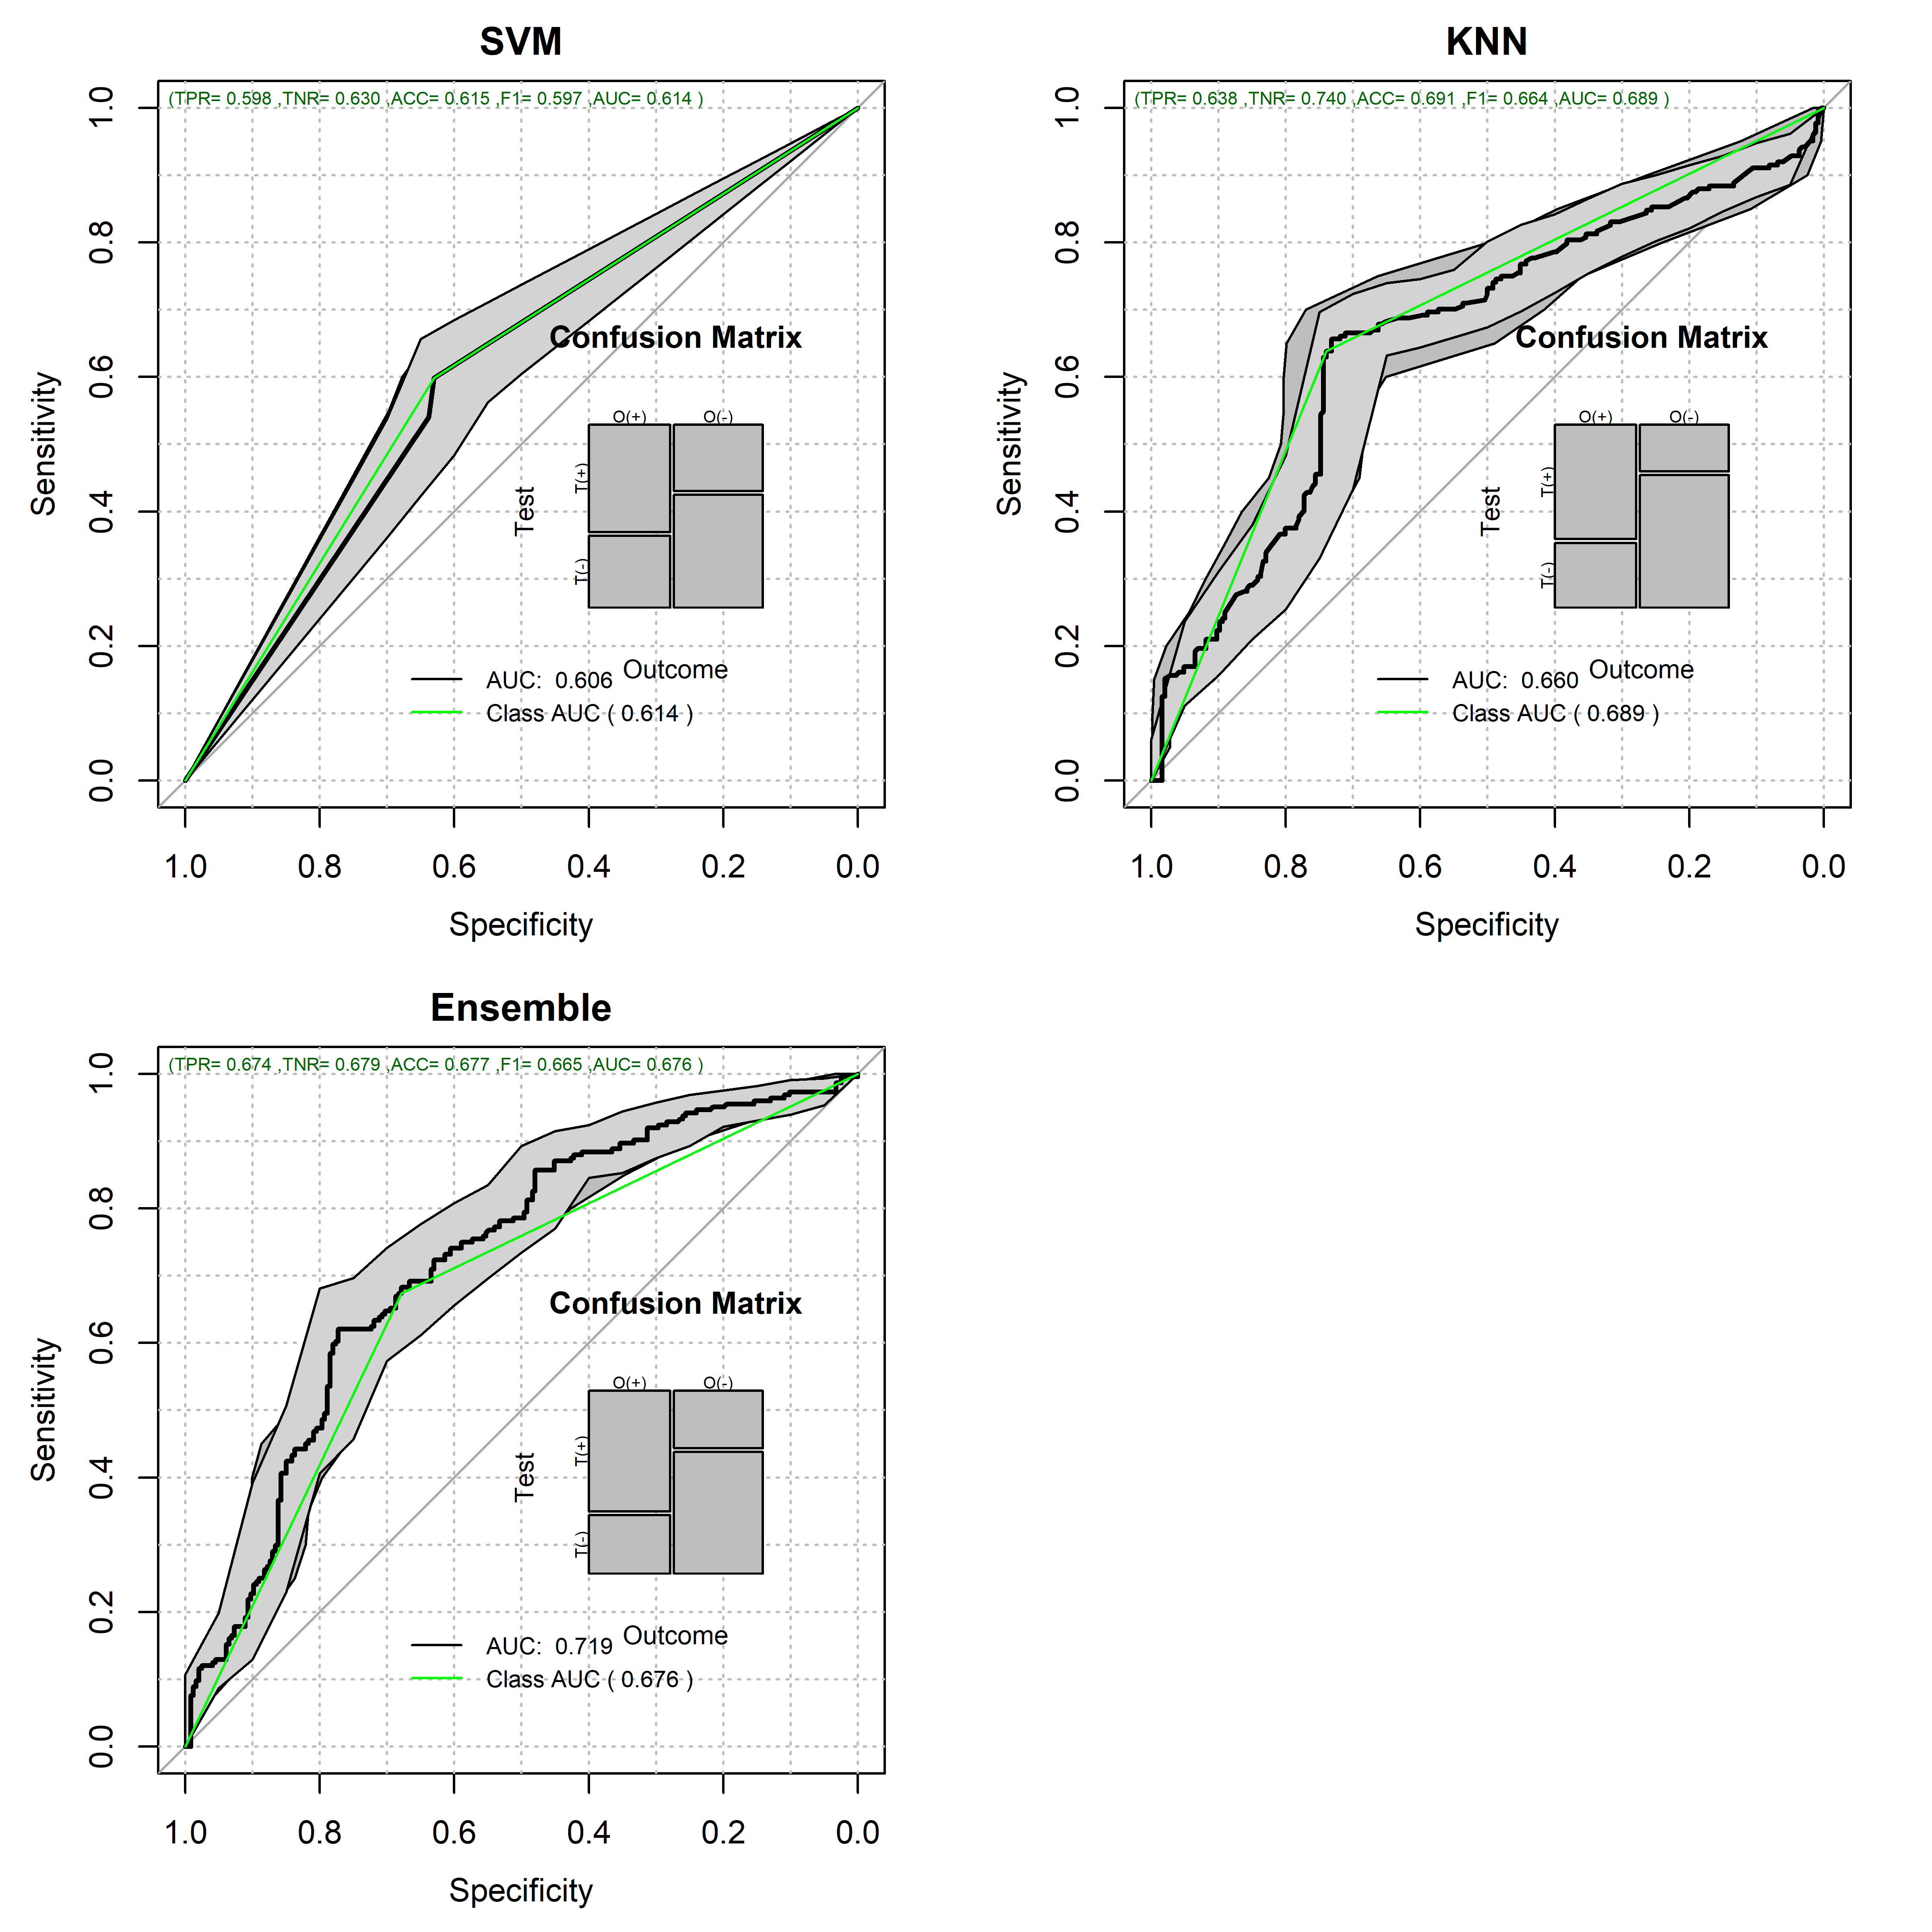
\includegraphics[width=3in]{images/results/fresaCurves2.png}}
\caption{{\bf ROC Curves for the FRESA.CAD Benchmarking Classifiers (Continued)} 
ROC Curves obtained using SVM, KNN and the Ensemble of the FRESA.CAD Benchmarking with the complete ADNI dataset for the Cross-Validation and the top 2,500 SNPs as inputs}
\label{fig141}
\end{figure}

The first characteristic to analyze with the benchmark is the similarity of classifiers across the classification. In figure 4.13 this is shown, and it can be observed that for cases and controls the values seem to be evenly classified for all SVMs, which means they are learning roughly the same variables and results. In the case of the LASSO it appears to be having trouble with some samples where there is not a clear difference (This can be seen in the Ensemble in a smaller manner). These methods are not entirely certain an individual belongs to either category. BSWIMS and KNN do classify some cases very strongly, but then do not perform that well in some other cases (Which could be due to selecting few features). The ensemble obtains a point in between these two groups which can be seen in the final results. In general it can be seen that in general the algorithms misclassify almost all of the same samples either for cases or for controls (Except the SVM with mRMR feature selection) and as such could give an idea of samples that either share characteristics that make them hard to classify, there is not enough information to further classify the problem or that they could be samples that could become cases in the future.
 
 \begin{figure}[!ht]
\centerline{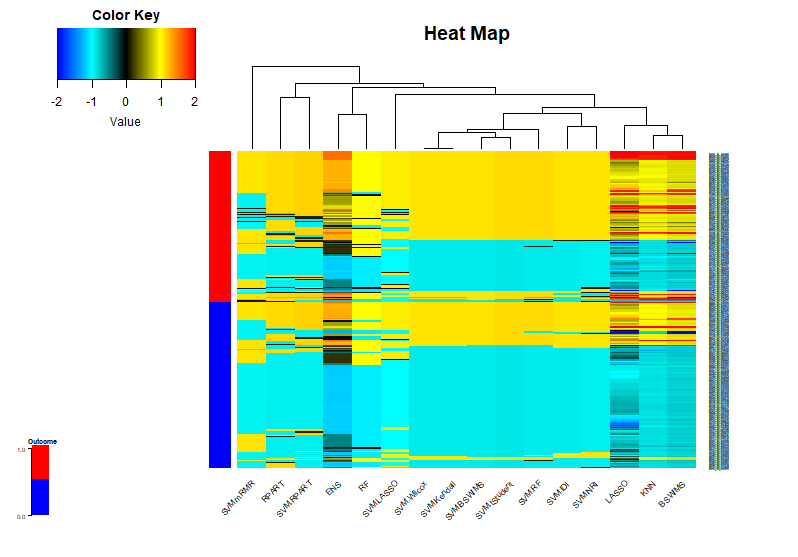
\includegraphics[width=3in]{images/results/fresaHM.png}}
\caption{{\bf Heatmap prediction comparison between FRESA.CAD Benchmark classifiers} 
Heatmap comparison of the prediction performance across classifiers. The Y axis describes each sample of the dataset with the real value (colour bar on the left) as well as the predicted value, while the X axis describes the different classifiers of the FRESA.CAD Benchmarking with the complete ADNI dataset for the Cross-validation and using the top 2,500 SNPs as input}
\label{fig15}
\end{figure}



In Figure 4.14 the Jaccard index is shown on the left; that is, the similarity between classifiers according to the features selected by each. In the dataset it can be observed that the BSWIMS has a high Jaccard Index and shows that the few features selected in that model are shared in more models. This makes sense as BSWiMS is choosing the APOE $\epsilon4$ gene as the main indicator, which has a high prediction power compared to all others and they do tend to choose it. As shown, an increase in the number of features (Right side of the figure) means that the Jaccard index starts to go lower as is the case for LASSO and RPART which are some of the best performers. The number of SNPs for these two models ranges from 30 to 75 SNPs, and as such it would seem using a higher number of SNPs could add additional information, although other models do use lower number of SNPs with good precision. There exists a balance that could show a number of variants in the range of decades is the best solution.

\begin{figure}[!ht]
\centerline{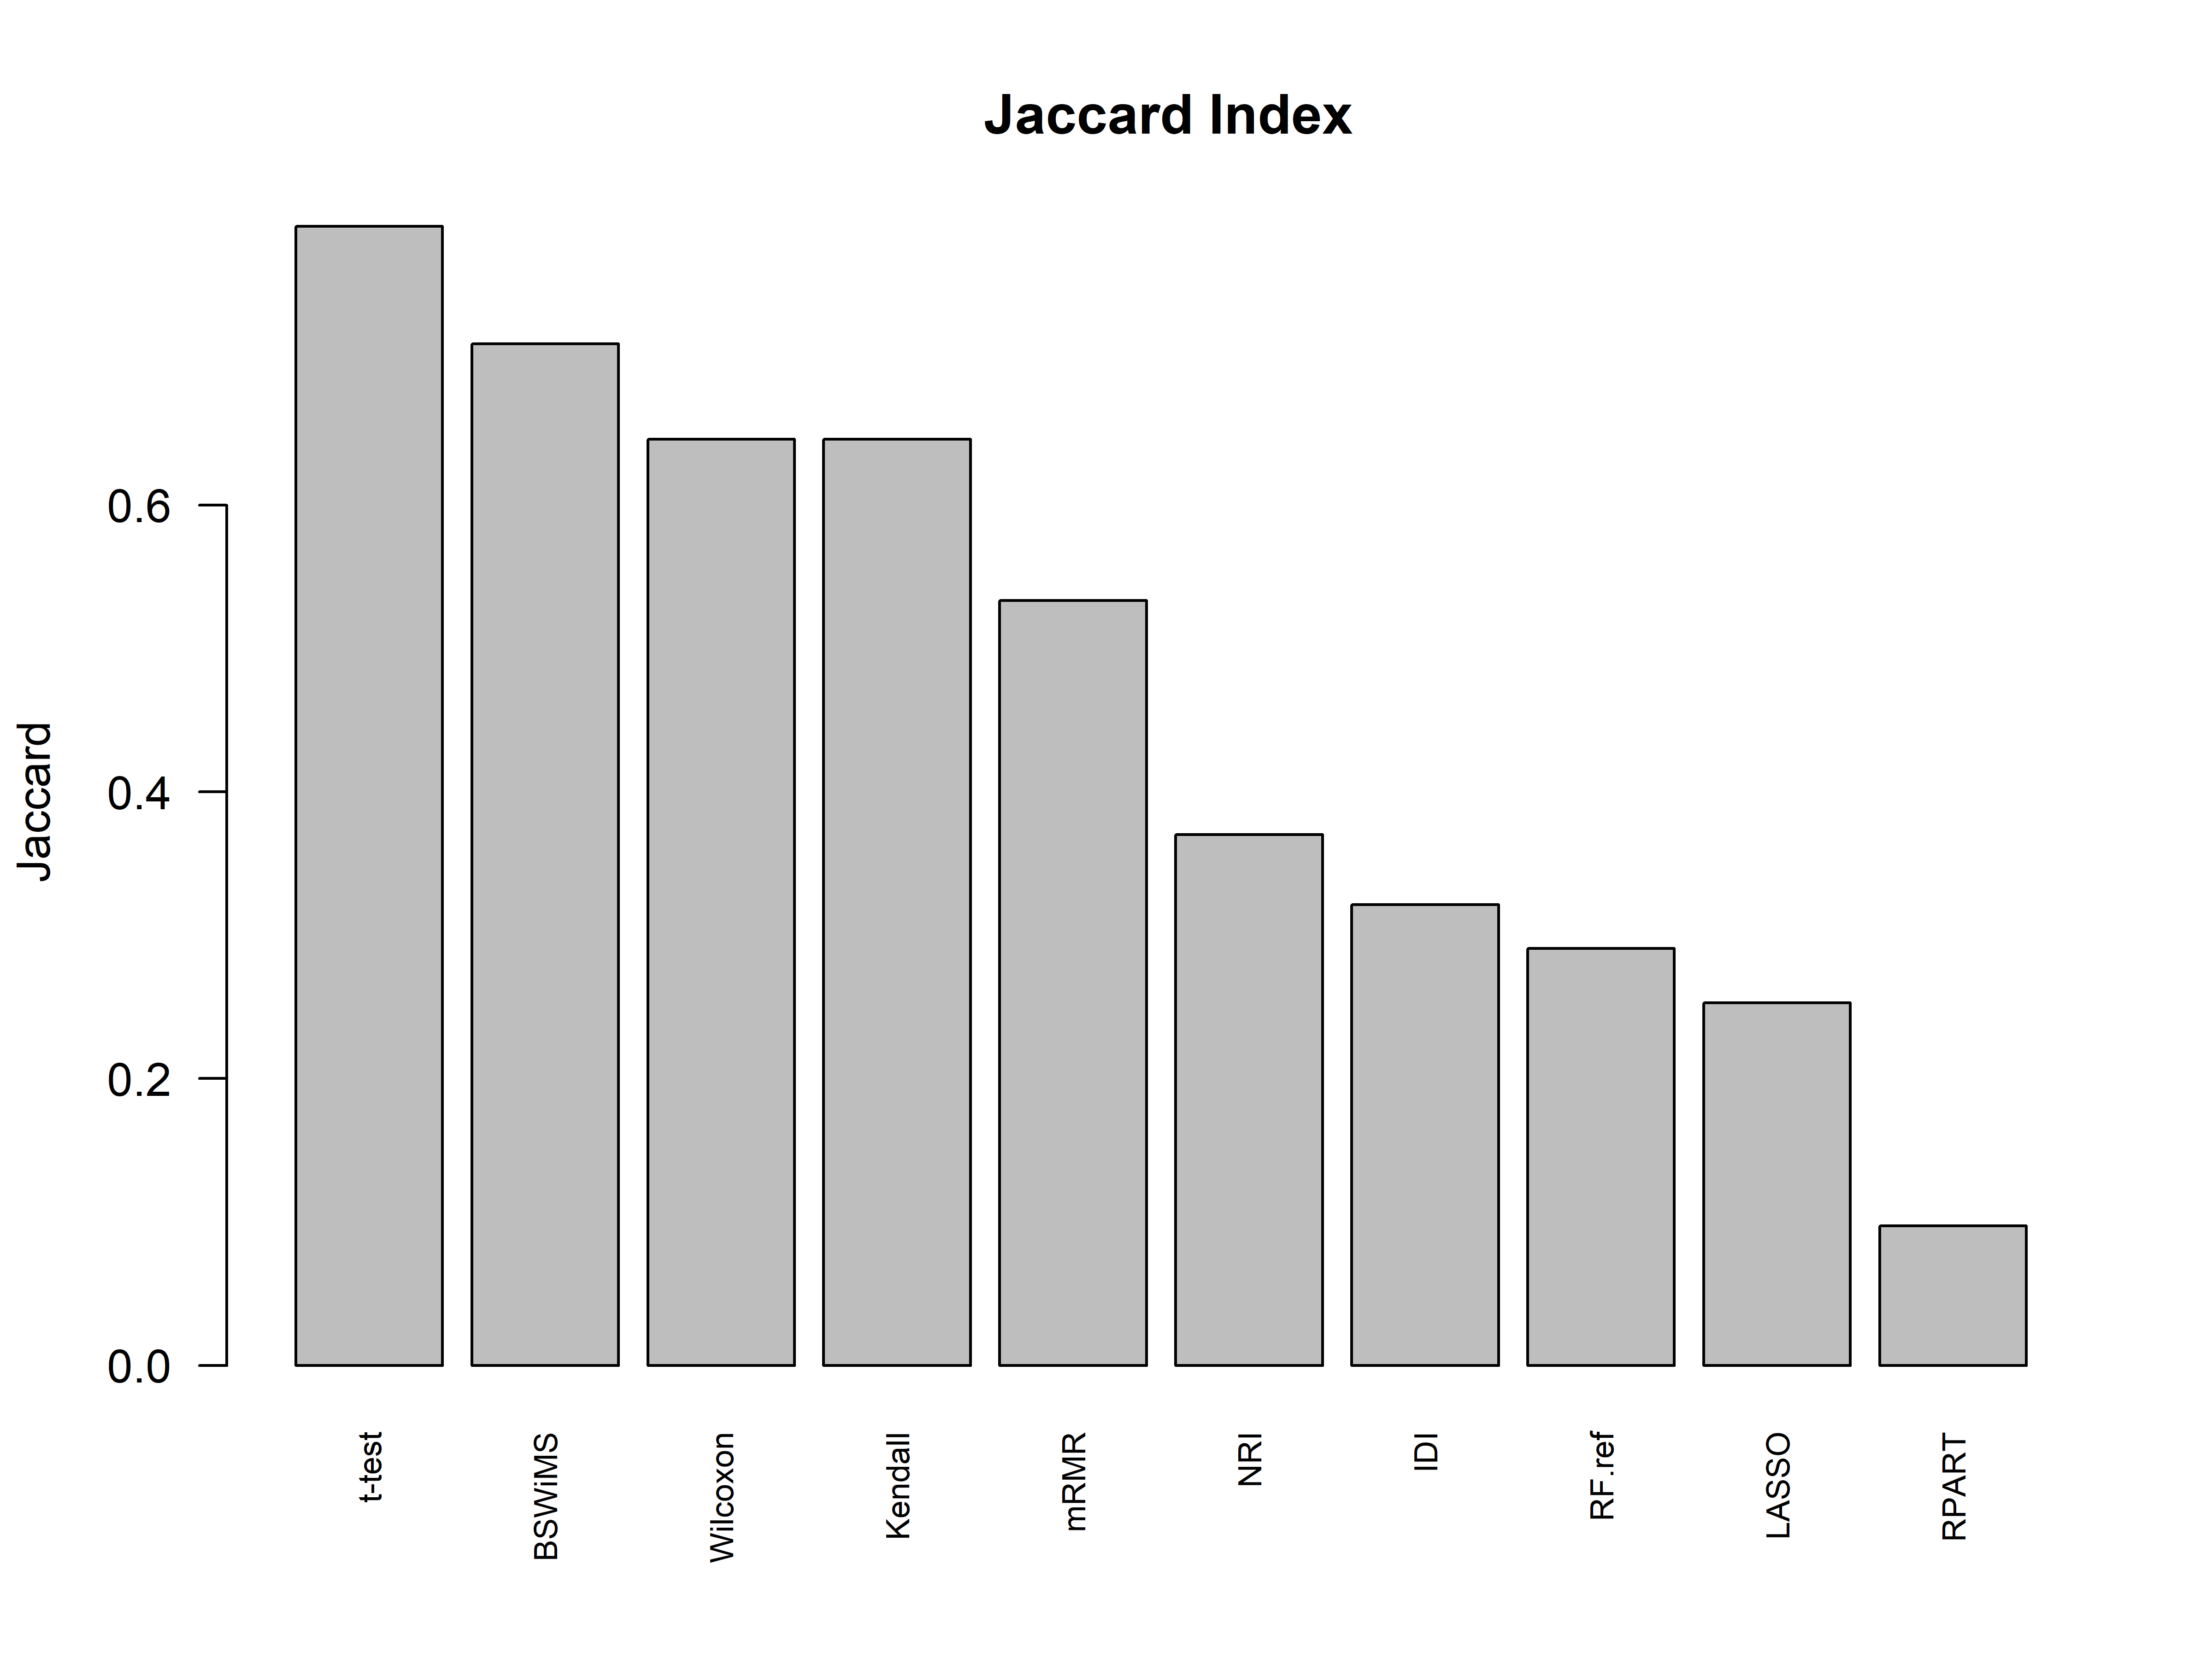
\includegraphics[width=2in]{images/results/fresaJac.png}}
\centerline{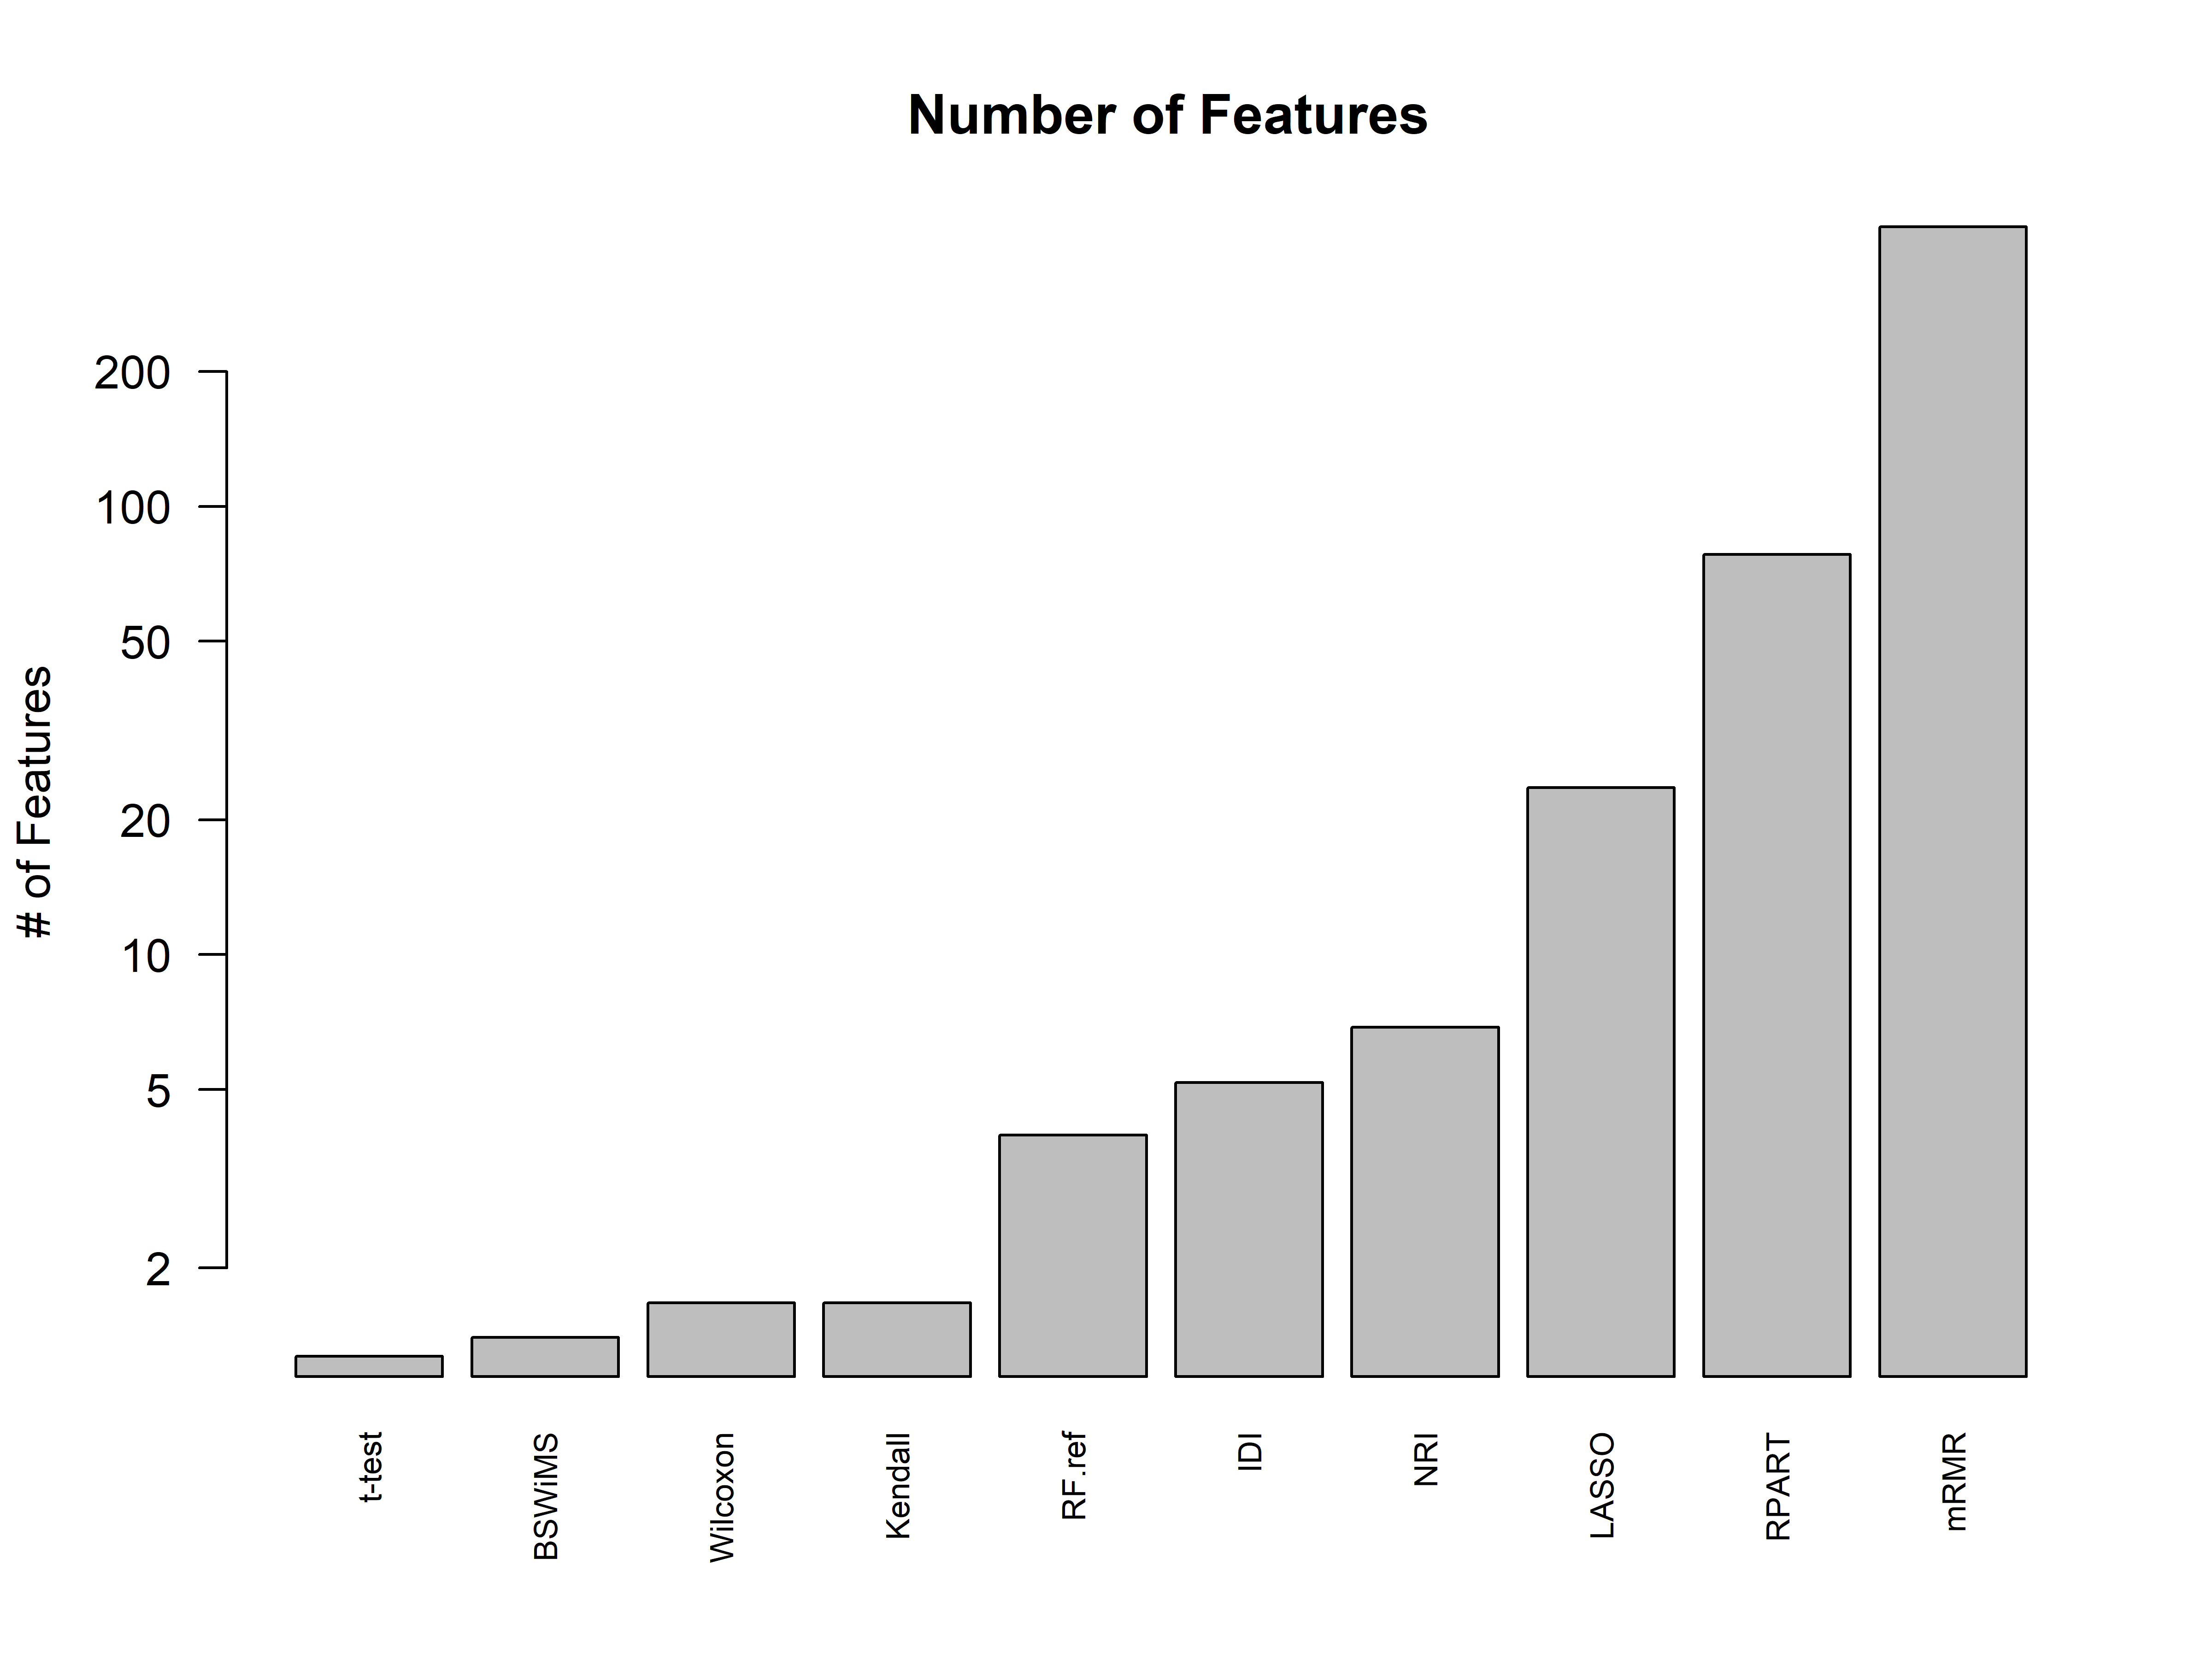
\includegraphics[width=2in]{images/results/fresaFeatures.png}}
\caption{{\bf Jaccard Index and Number of Features} 
Jaccard Index metric of the different classifiers between features selected as well as the number of features selected by each classifier of the FRESA.CAD Benchmarking with the complete ADNI dataset for the Cross-validation and using the top 2,500 SNPs as input }
\label{fig16}
\end{figure}
\newpage
With Figure 4.15 and 4.16 the analysis can be further expanded to see the balanced Error, AUC, Accuracy as well as Specificity and Sensitivity for both classifiers and the combinations with filters. As expected, BSWiMS performs quite well in the Balanced Error and the other metrics, then the ensemble, while RPART and LASSO perform slightly worse. In the filters the Random Forest filter gives the best results for the ROC, while some other filters such as Spearman or KNN perform well in just one of the two cases, as such it might be better to use certain combinations depending on the importance of detecting a case or a control more precisely. And thanks to the confidence intervals given it can be seen that only SVMs would perform worse than the others. This supports the idea seen in the heatmap analysis.
\clearpage
 \begin{figure}[!ht]
\centerline{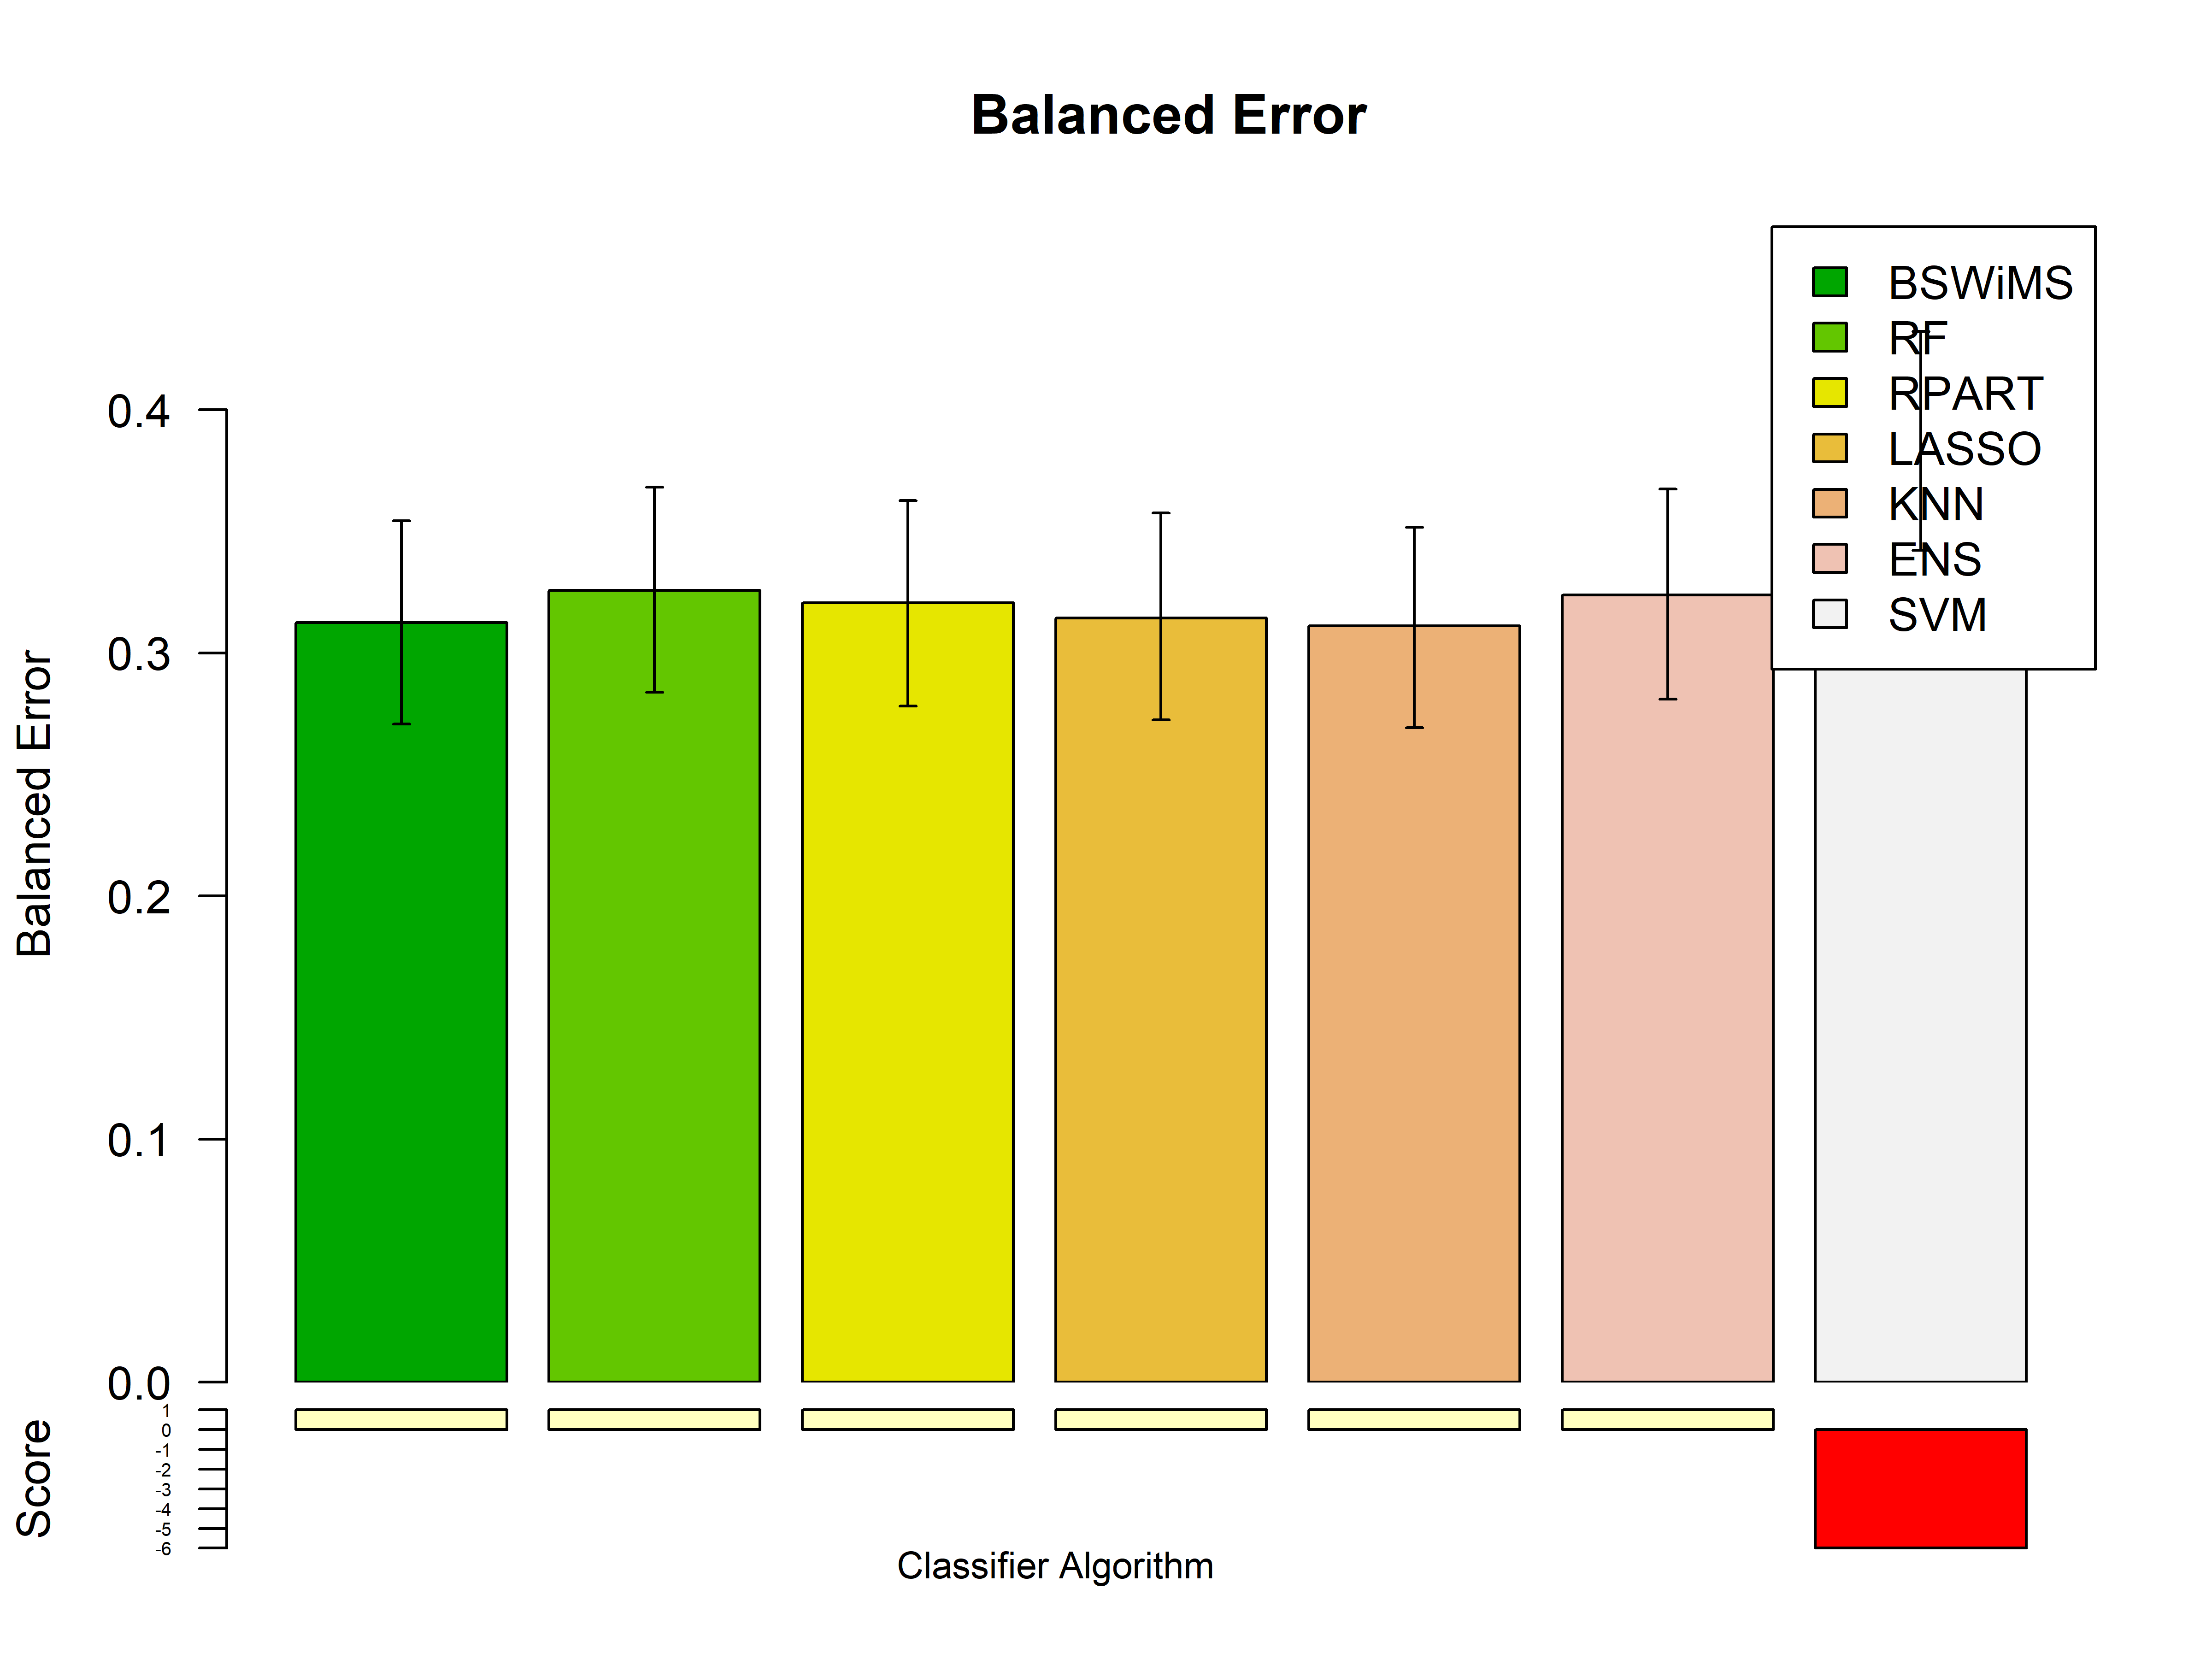
\includegraphics[width=5in,height=2in]{images/results/fresaBE.png}}
\centerline{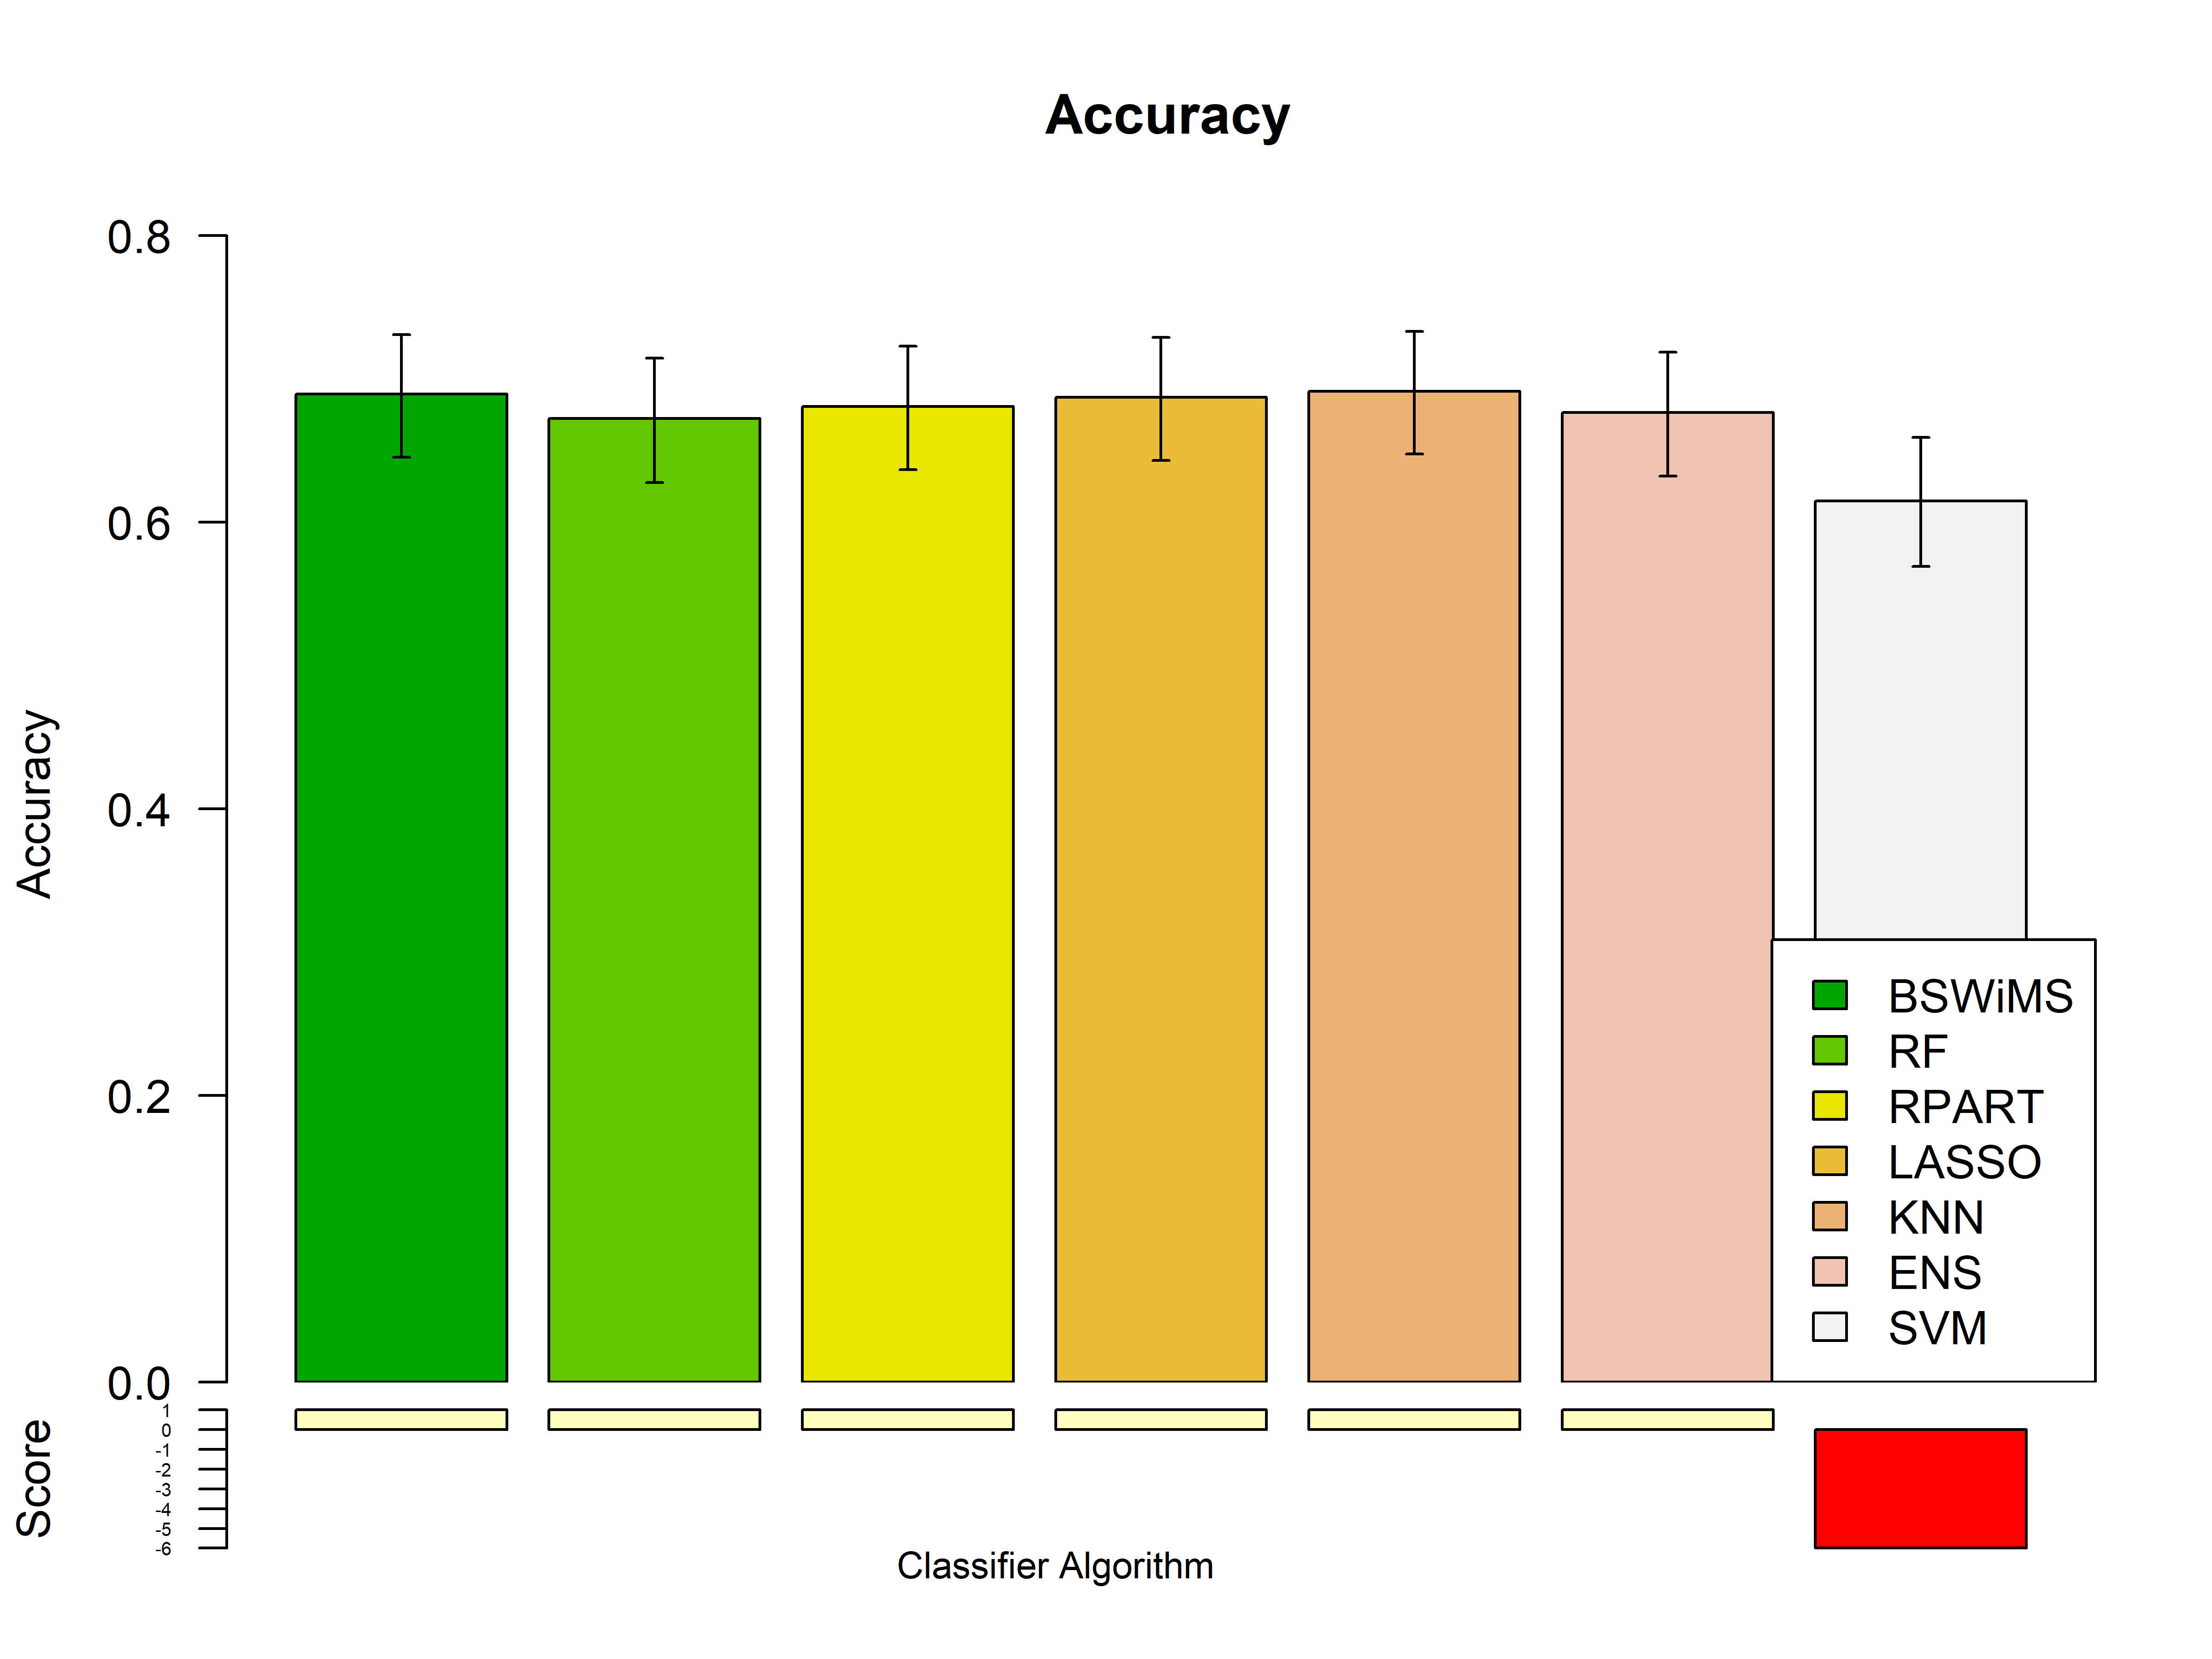
\includegraphics[width=5in,height=2in]{images/results/fresaAcc.png}}
\centerline{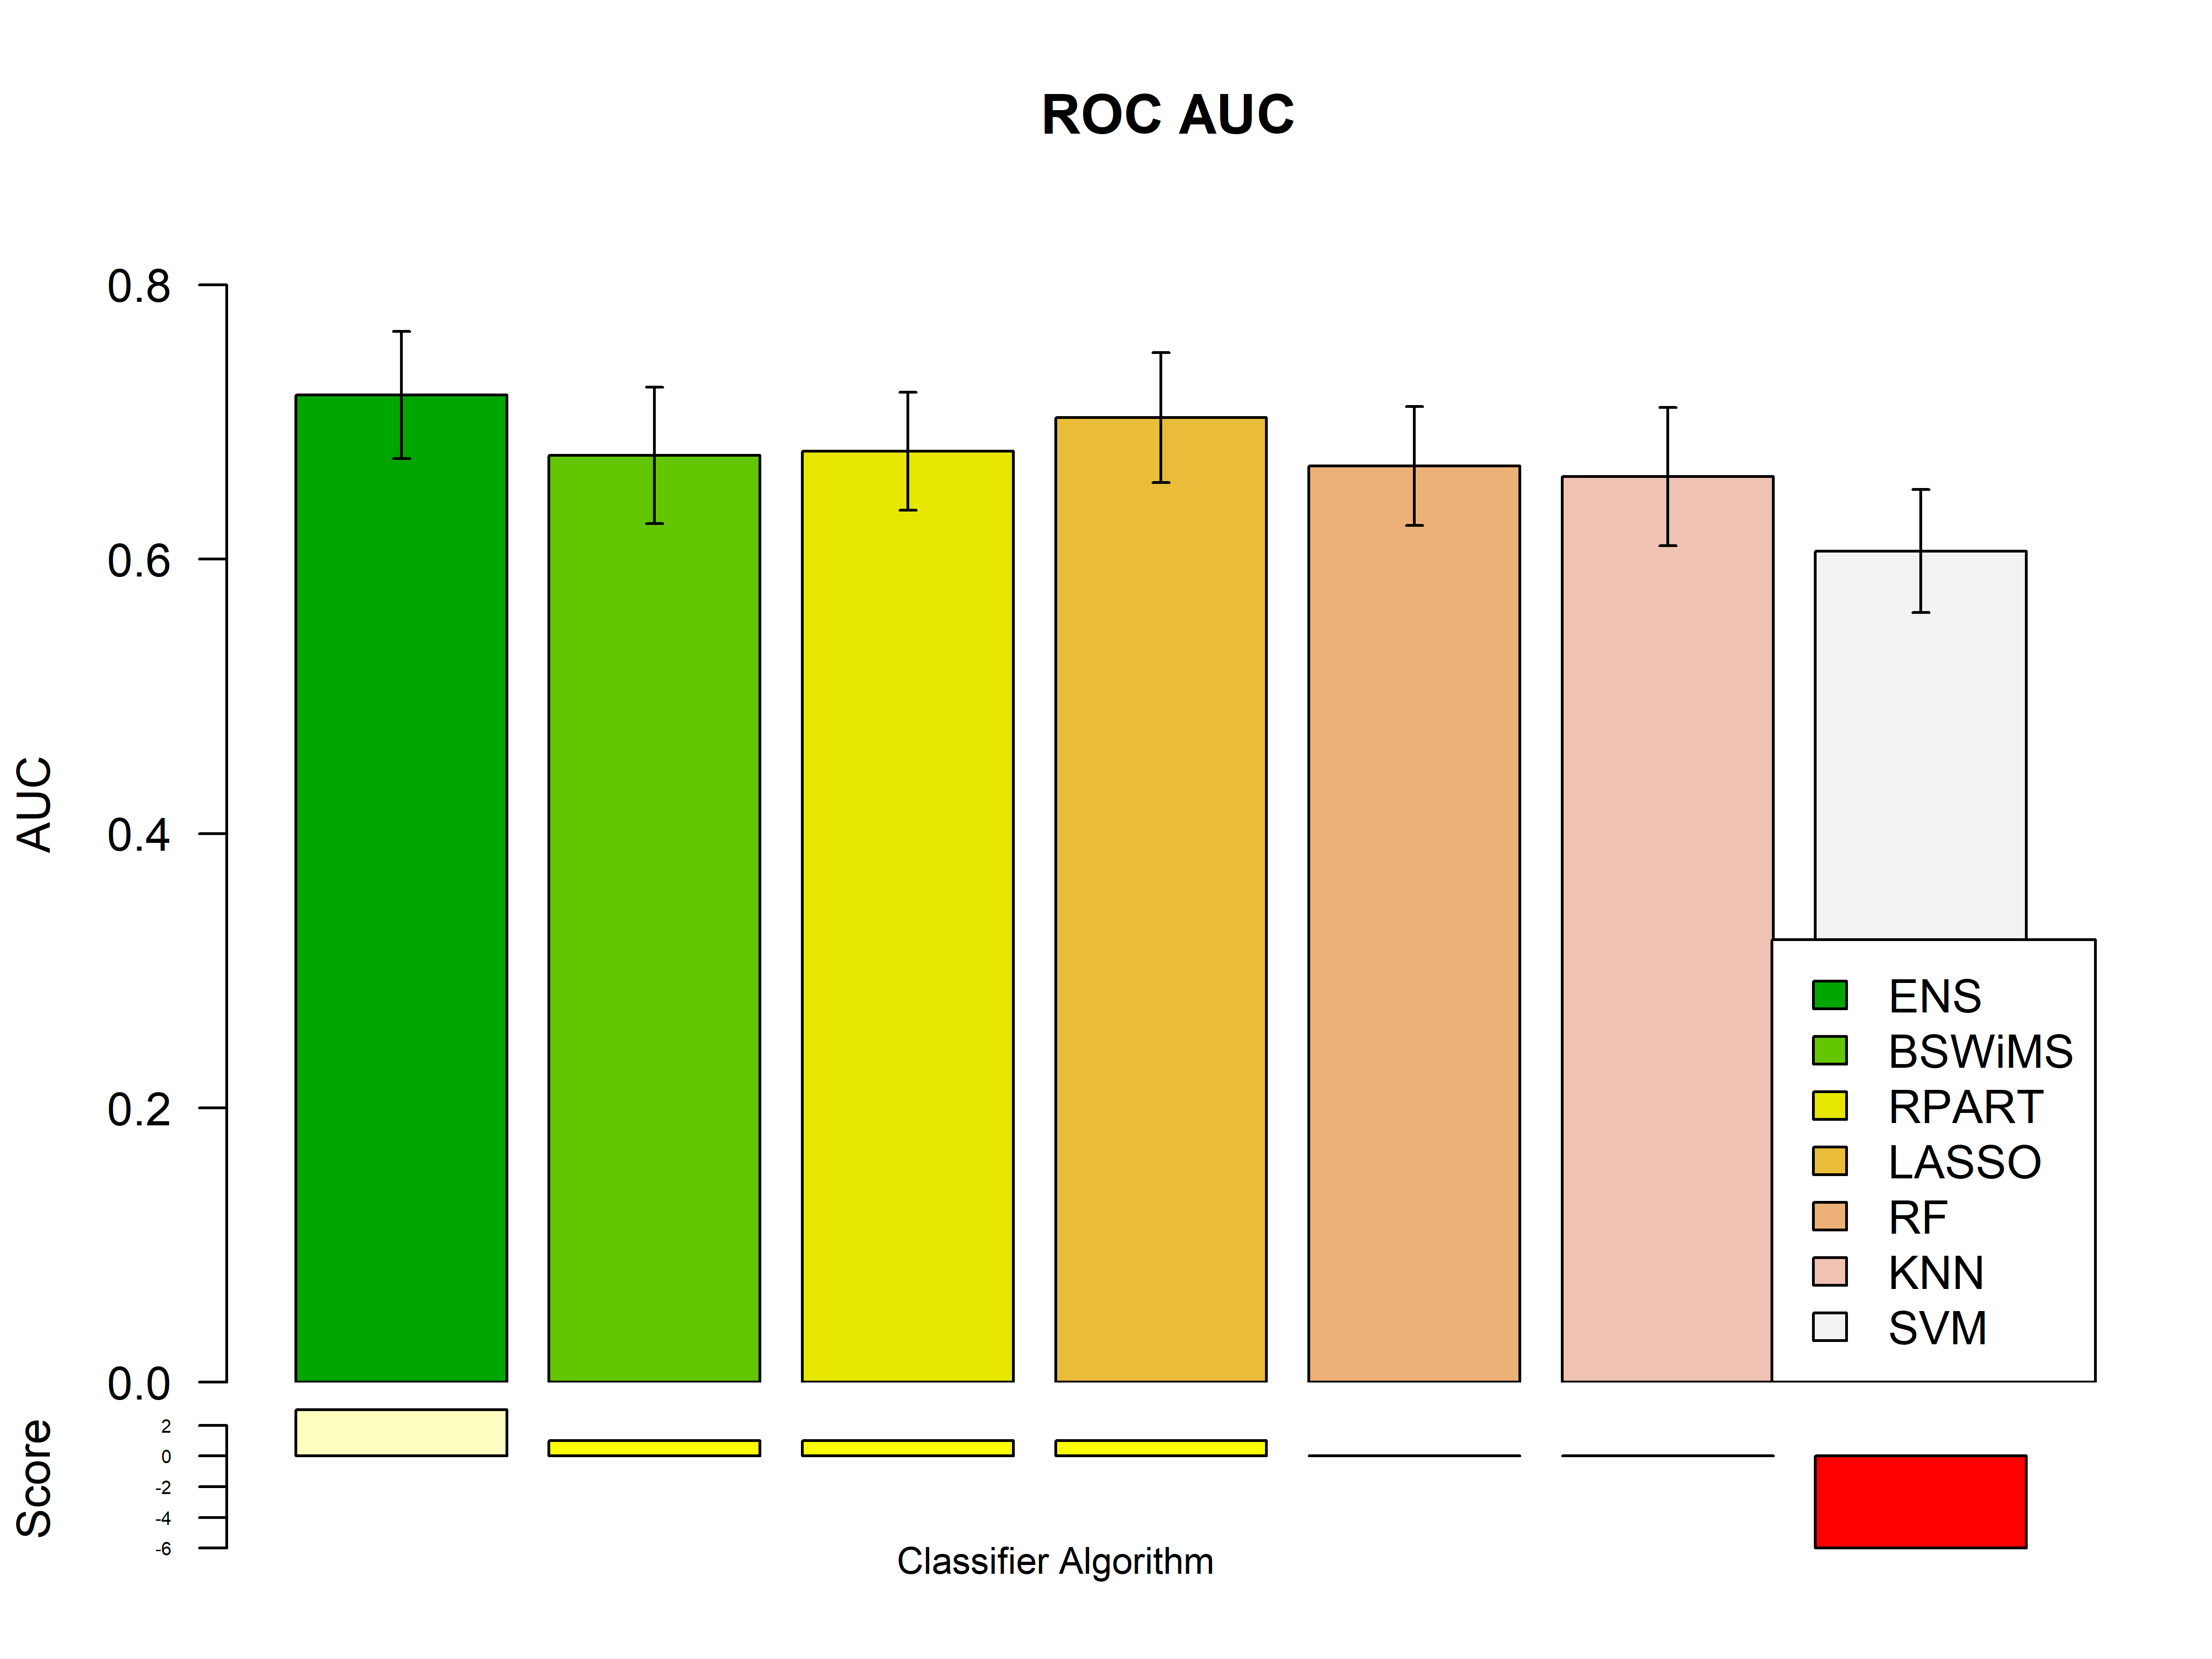
\includegraphics[width=5in,height=2in]{images/results/fresaAUC.png}}
\caption{{\bf Balanced Error, Accuracy and AUC of the FRESA.CAD Benchmark classifiers} 
Comparison between the Balanced Error, Accuracy and AUC Score obtained using the different classification methods of the FRESA.CAD Benchmarking with the complete ADNI dataset for the Cross-validation and using the top 2,500 SNPs as input}
\label{fig17}
\end{figure}

   
\begin{figure}[!ht]
\centerline{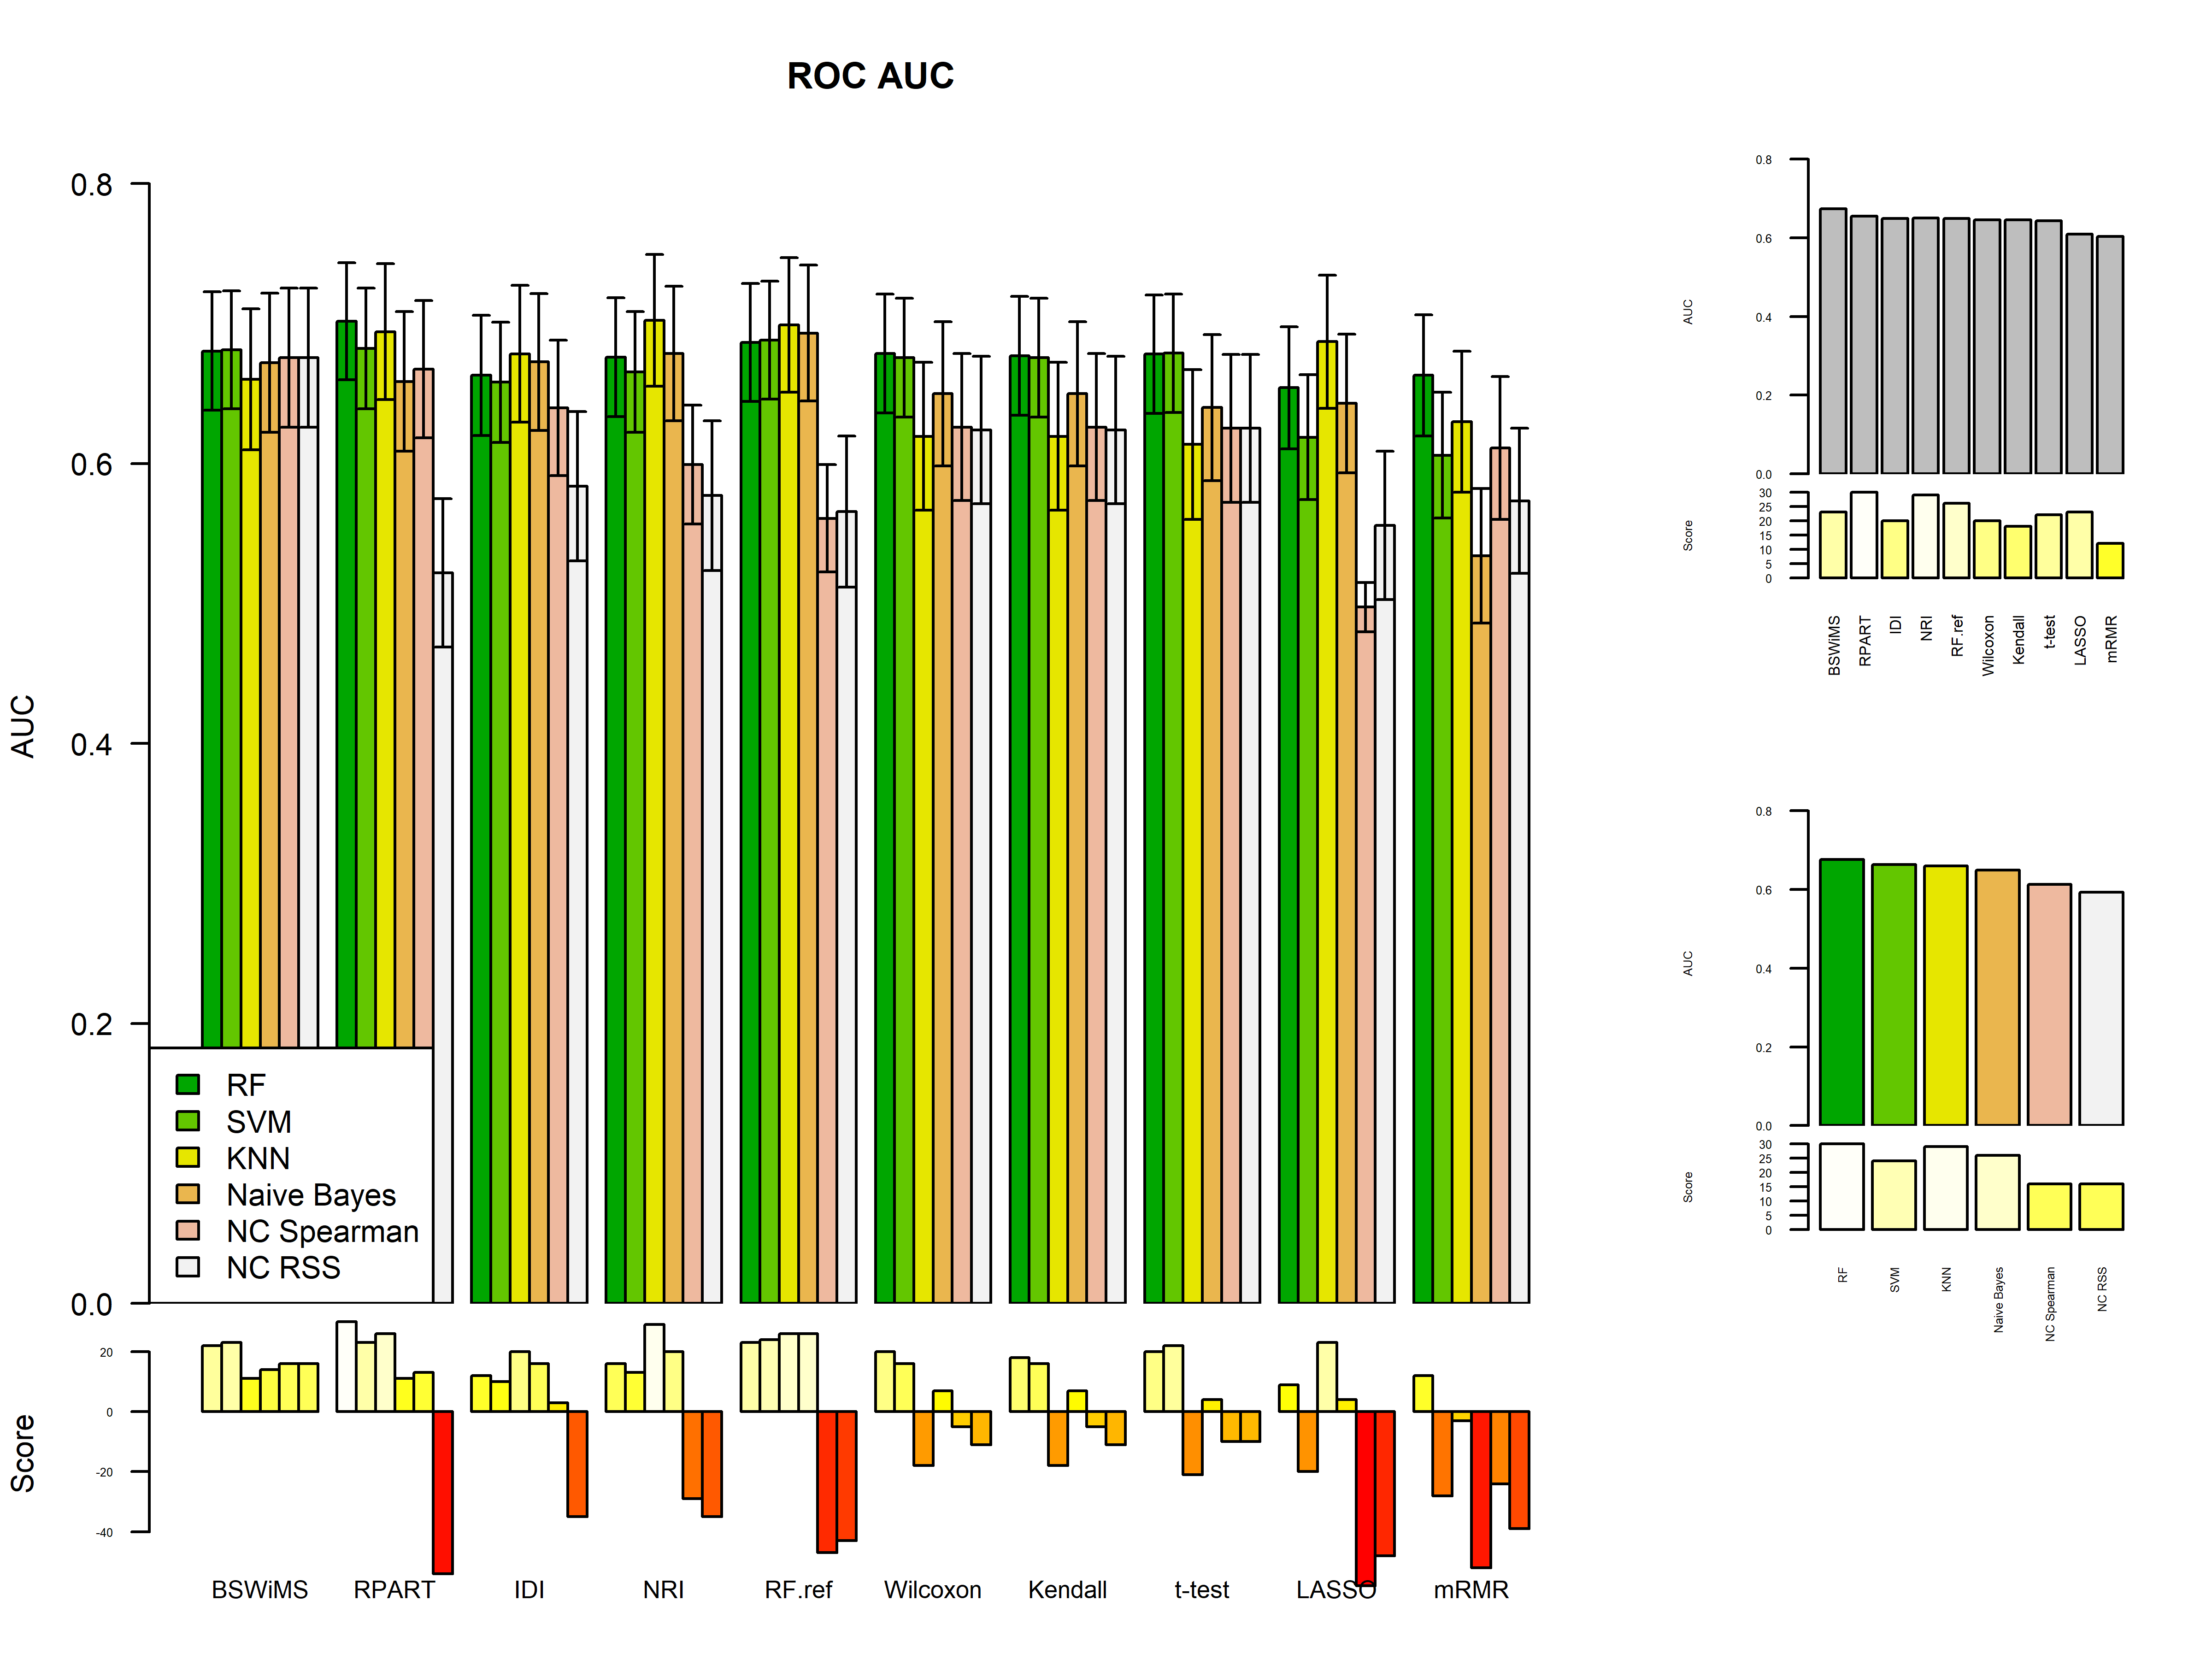
\includegraphics[width=5in,height=2in]{images/results/fresaConc.png}}
\centerline{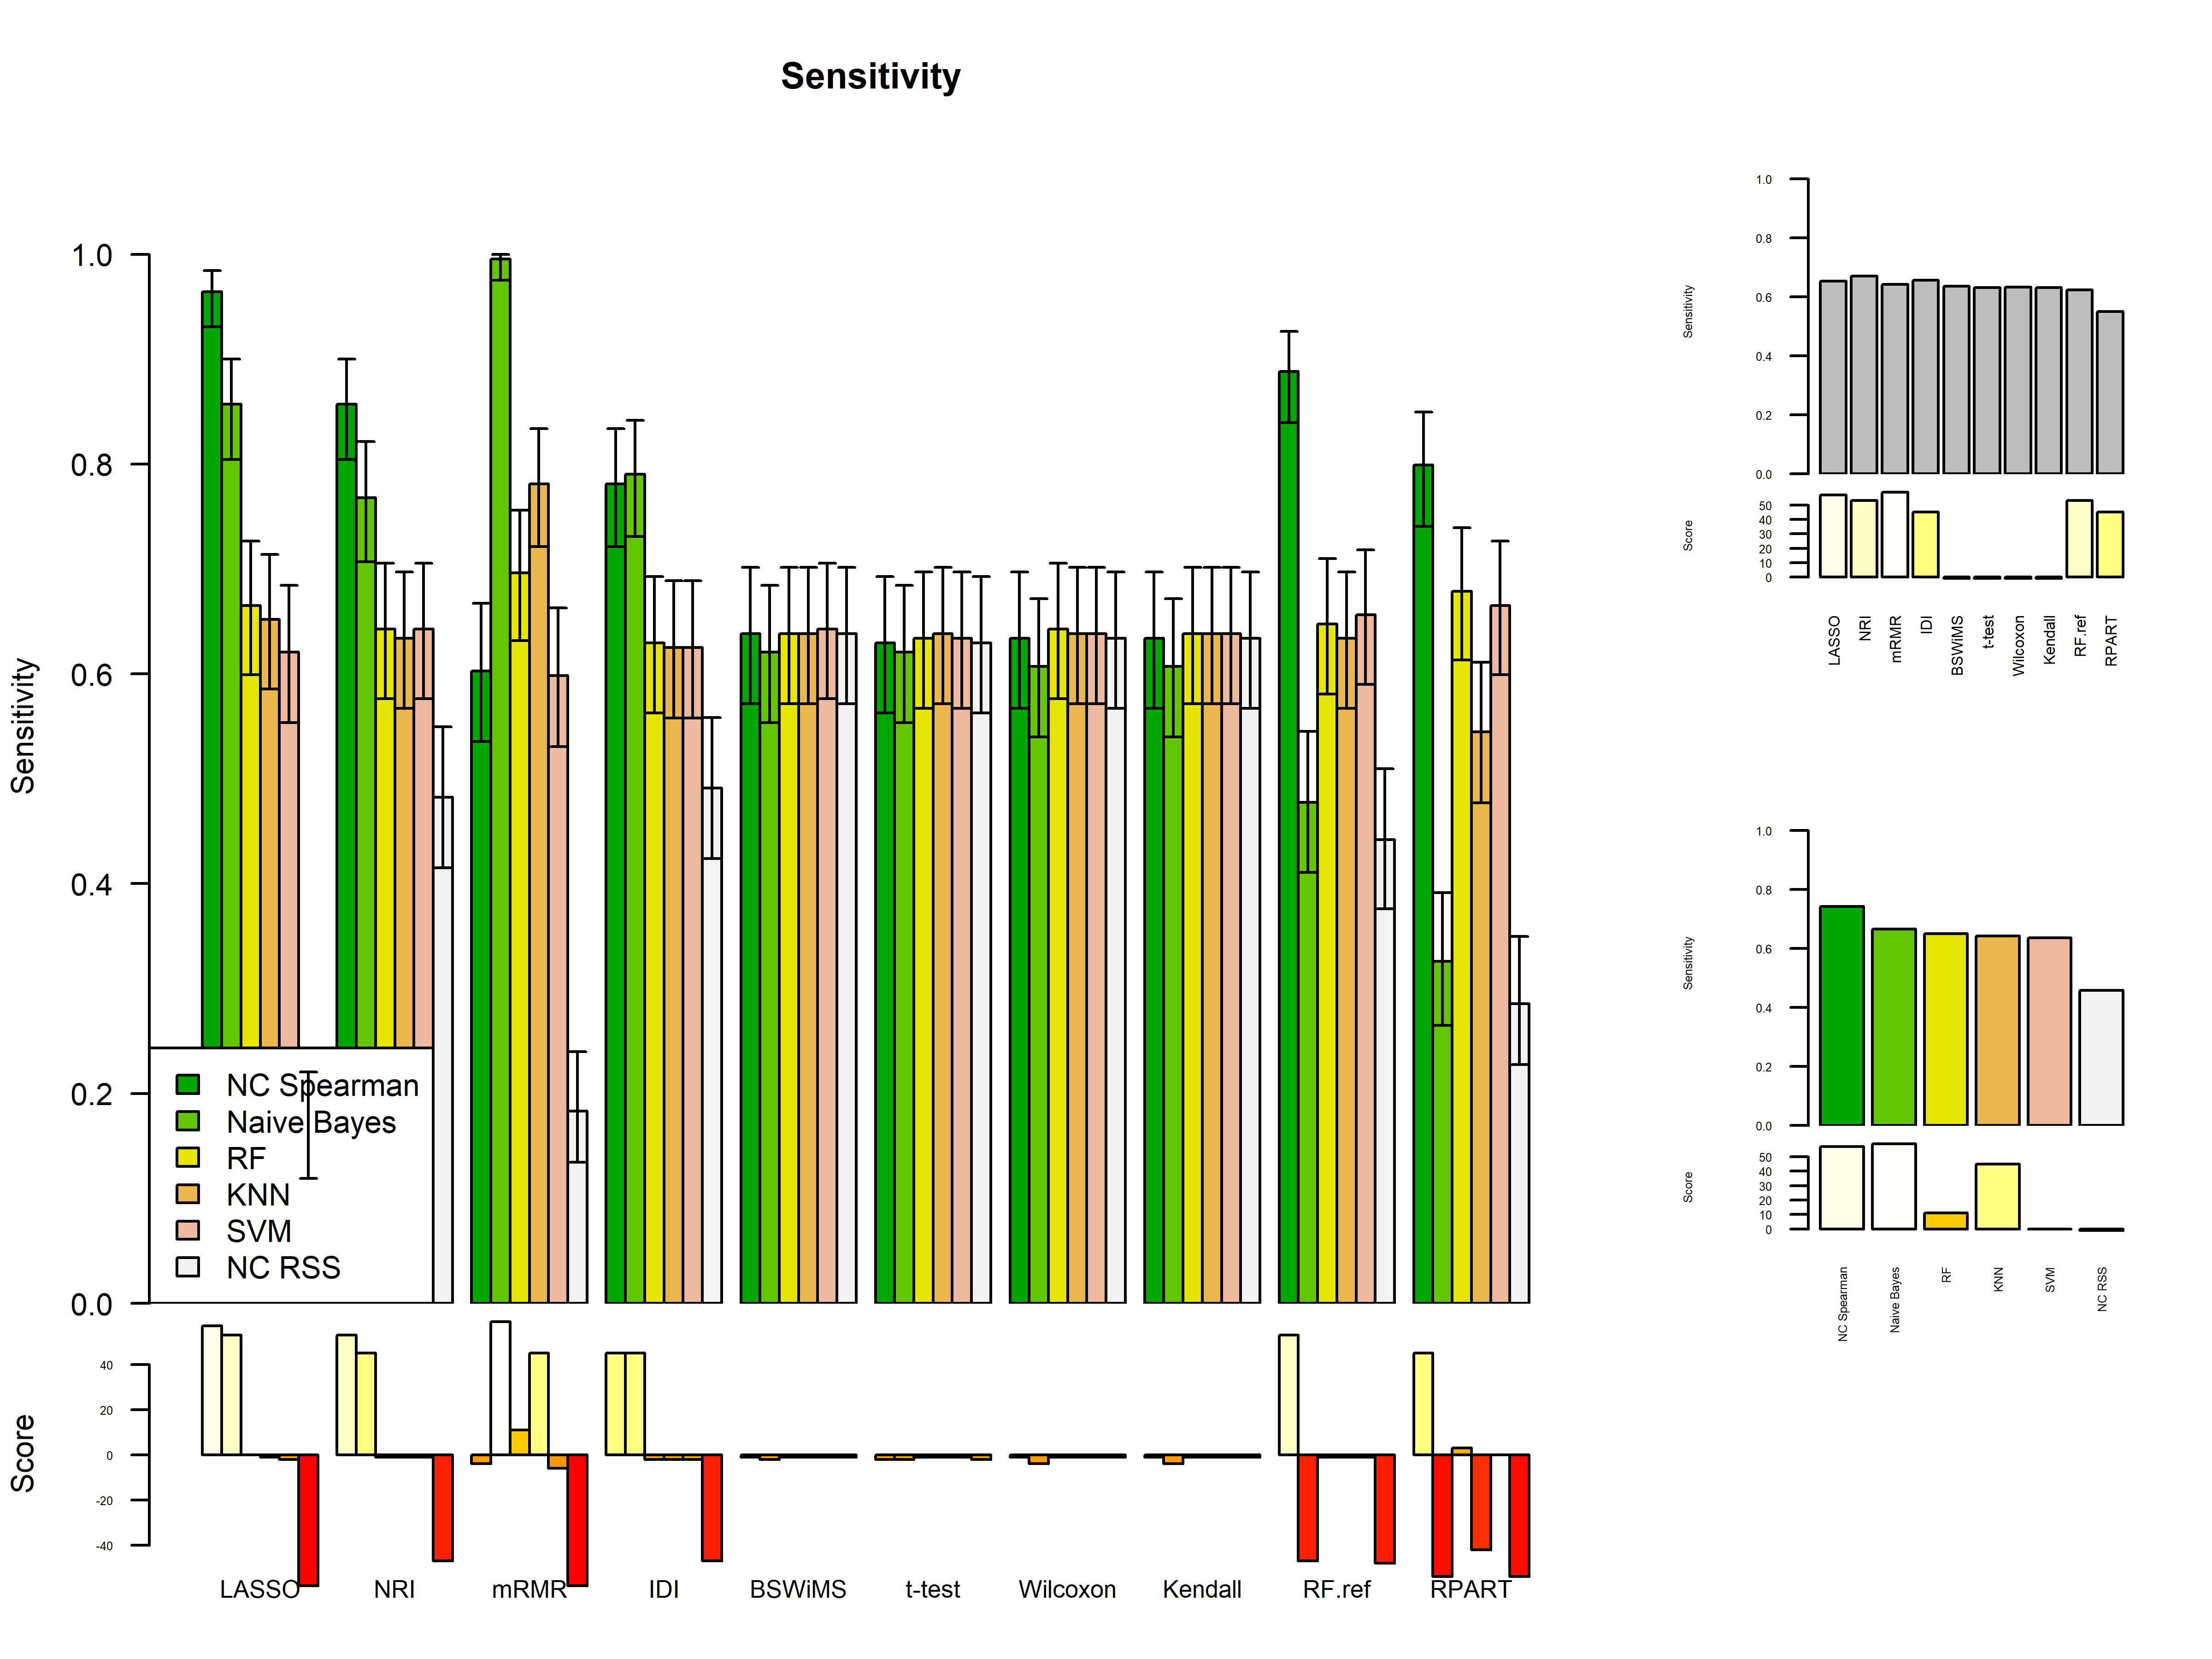
\includegraphics[width=5in,height=2in]{images/results/fresaSens.png}}
\centerline{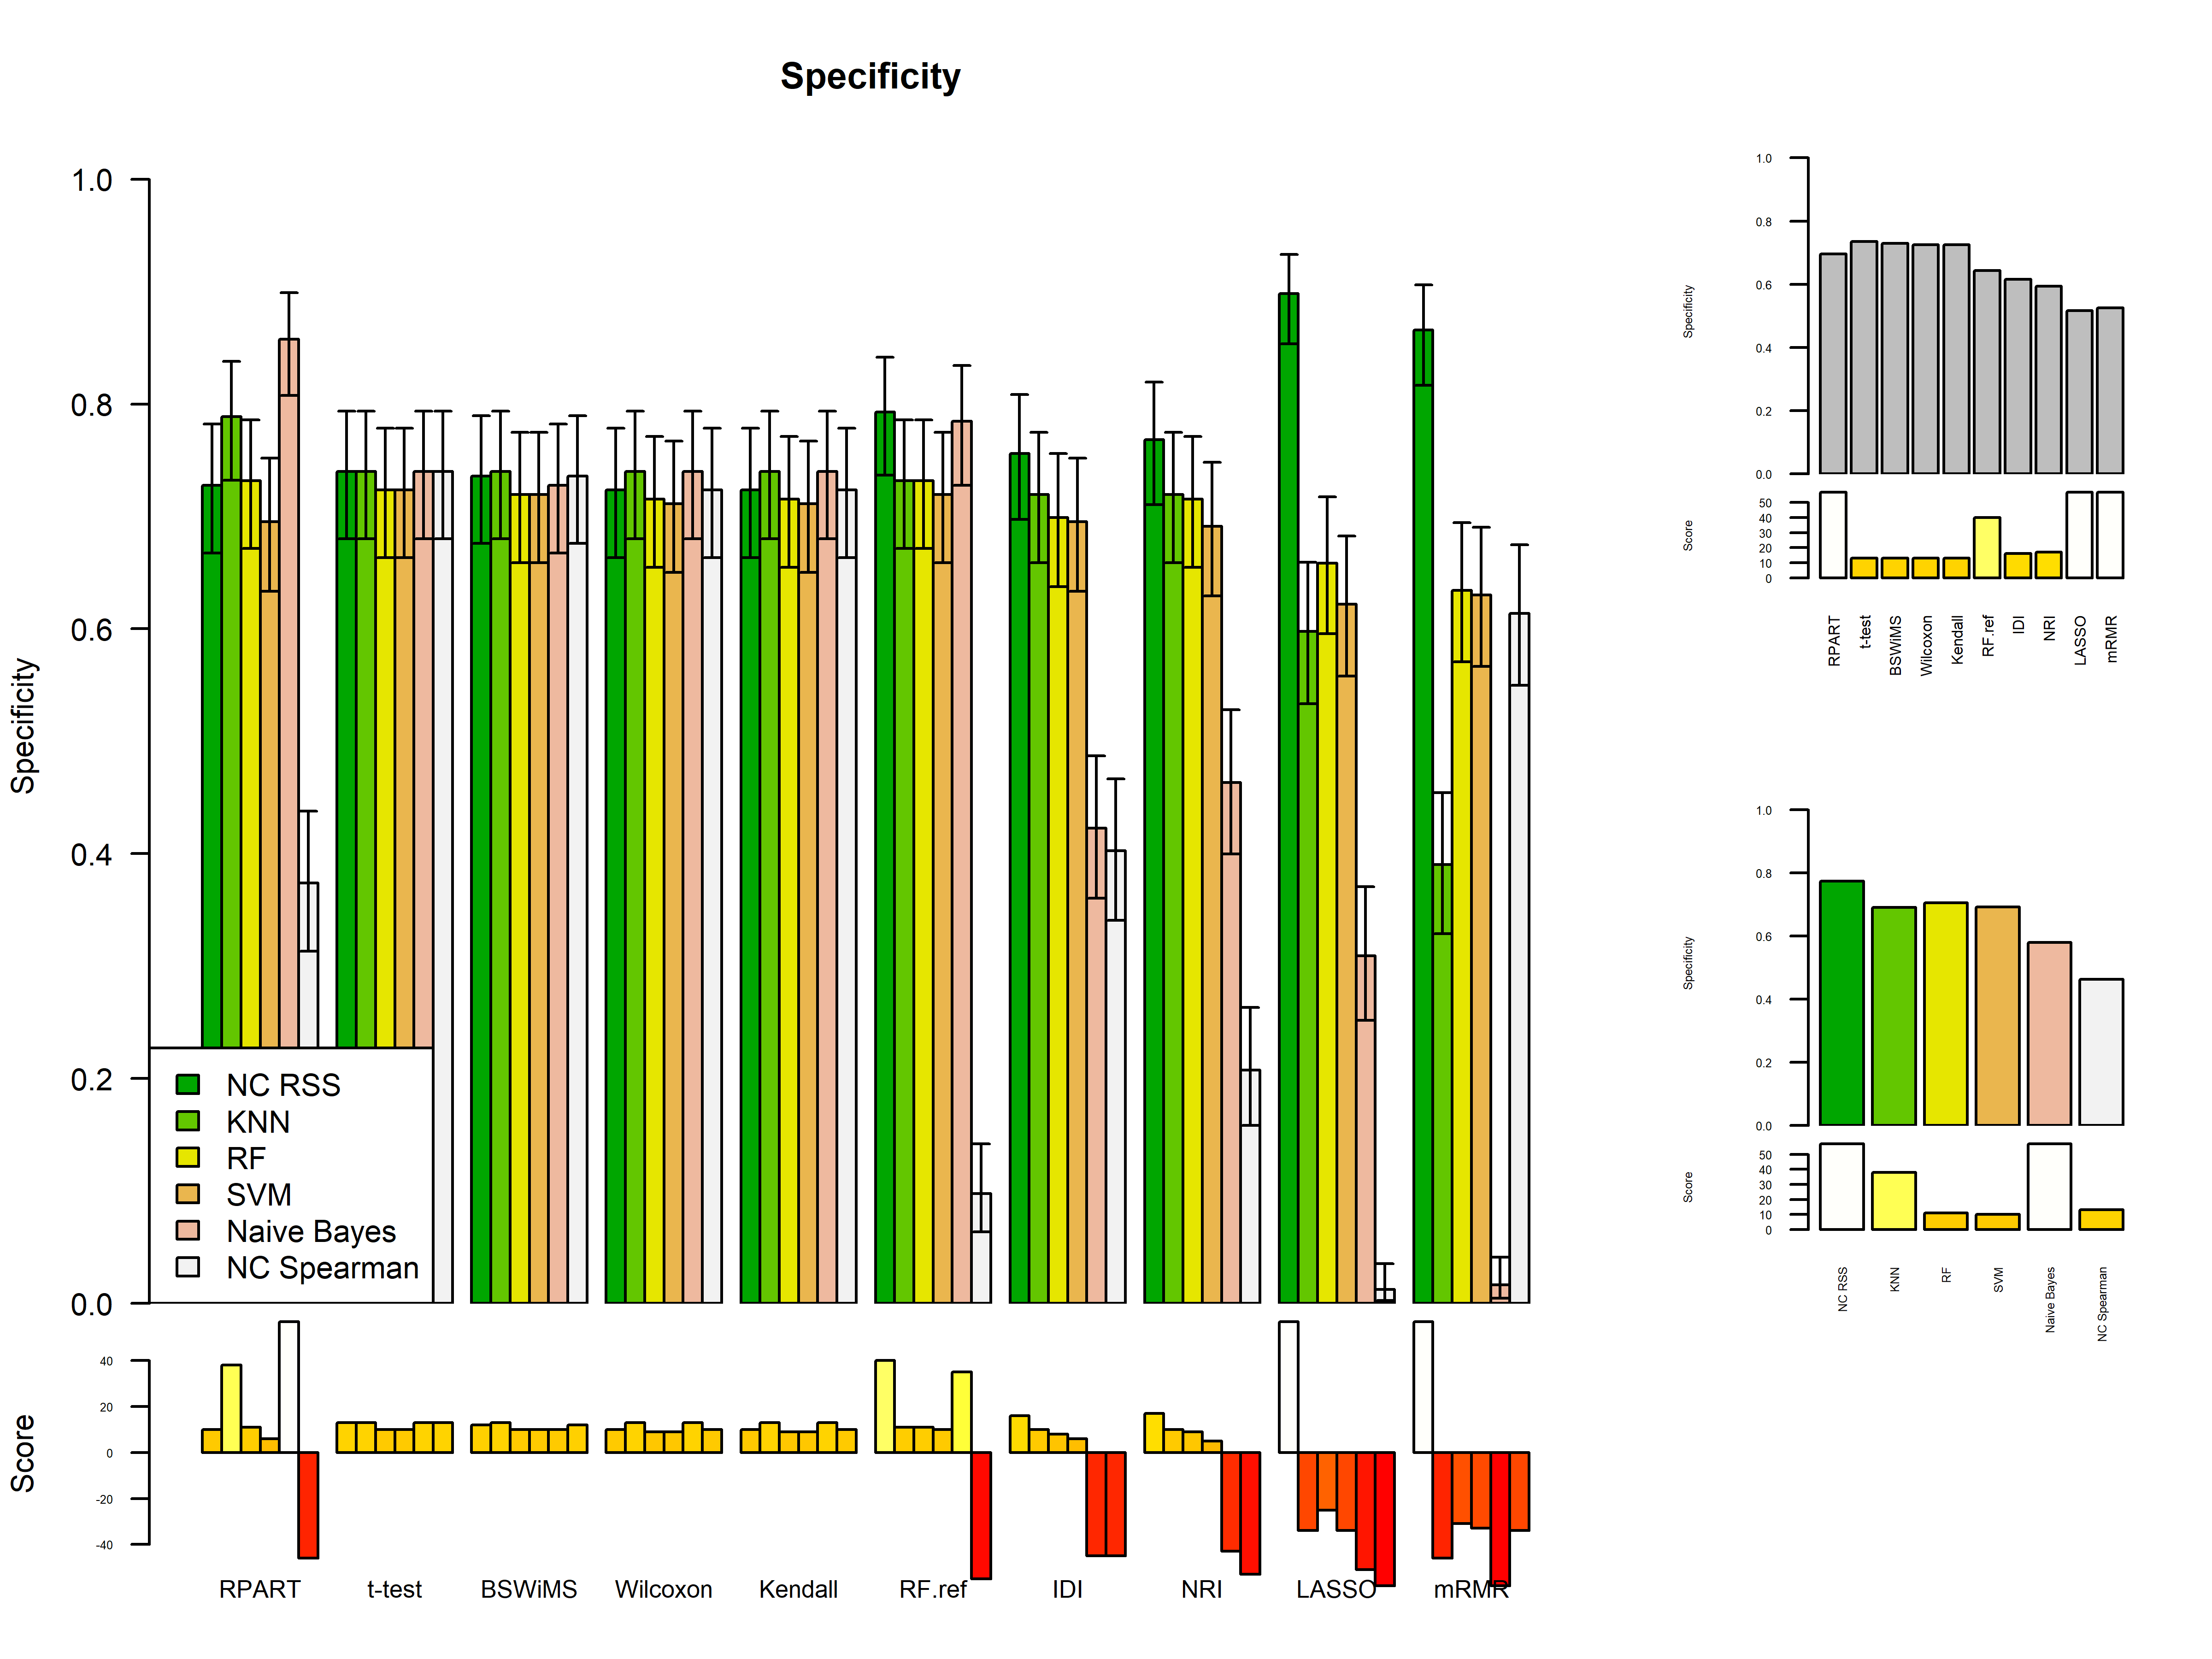
\includegraphics[width=5in,height=2in]{images/results/fresaSpec.png}}
\caption{{\bf ROC AUC, Sensitivity and Specificity of the FRESA.CAD Filter combinations} 
Comparison the ROC AUC, Sensitivity and Specificity Score obtained using the different combinations of classification methods plus filters of the FRESA.CAD Benchmarking with the complete ADNI dataset for the Cross-validation and using the top 2,500 SNPs as input}
\label{fig18}
\end{figure}
\newpage
A balanced comparison across metrics for the different classifiers can be seen in Figure 4.17. For the prediction models they all roughly perform the same with just the SVM varying from the others, but on the Filter method it can be seen how mRMR, Lasso, and RF filter give a worse Balanced Error than the others. BSWiMS features appear to be the best all around filter method.

\begin{figure}[!ht]
\centerline{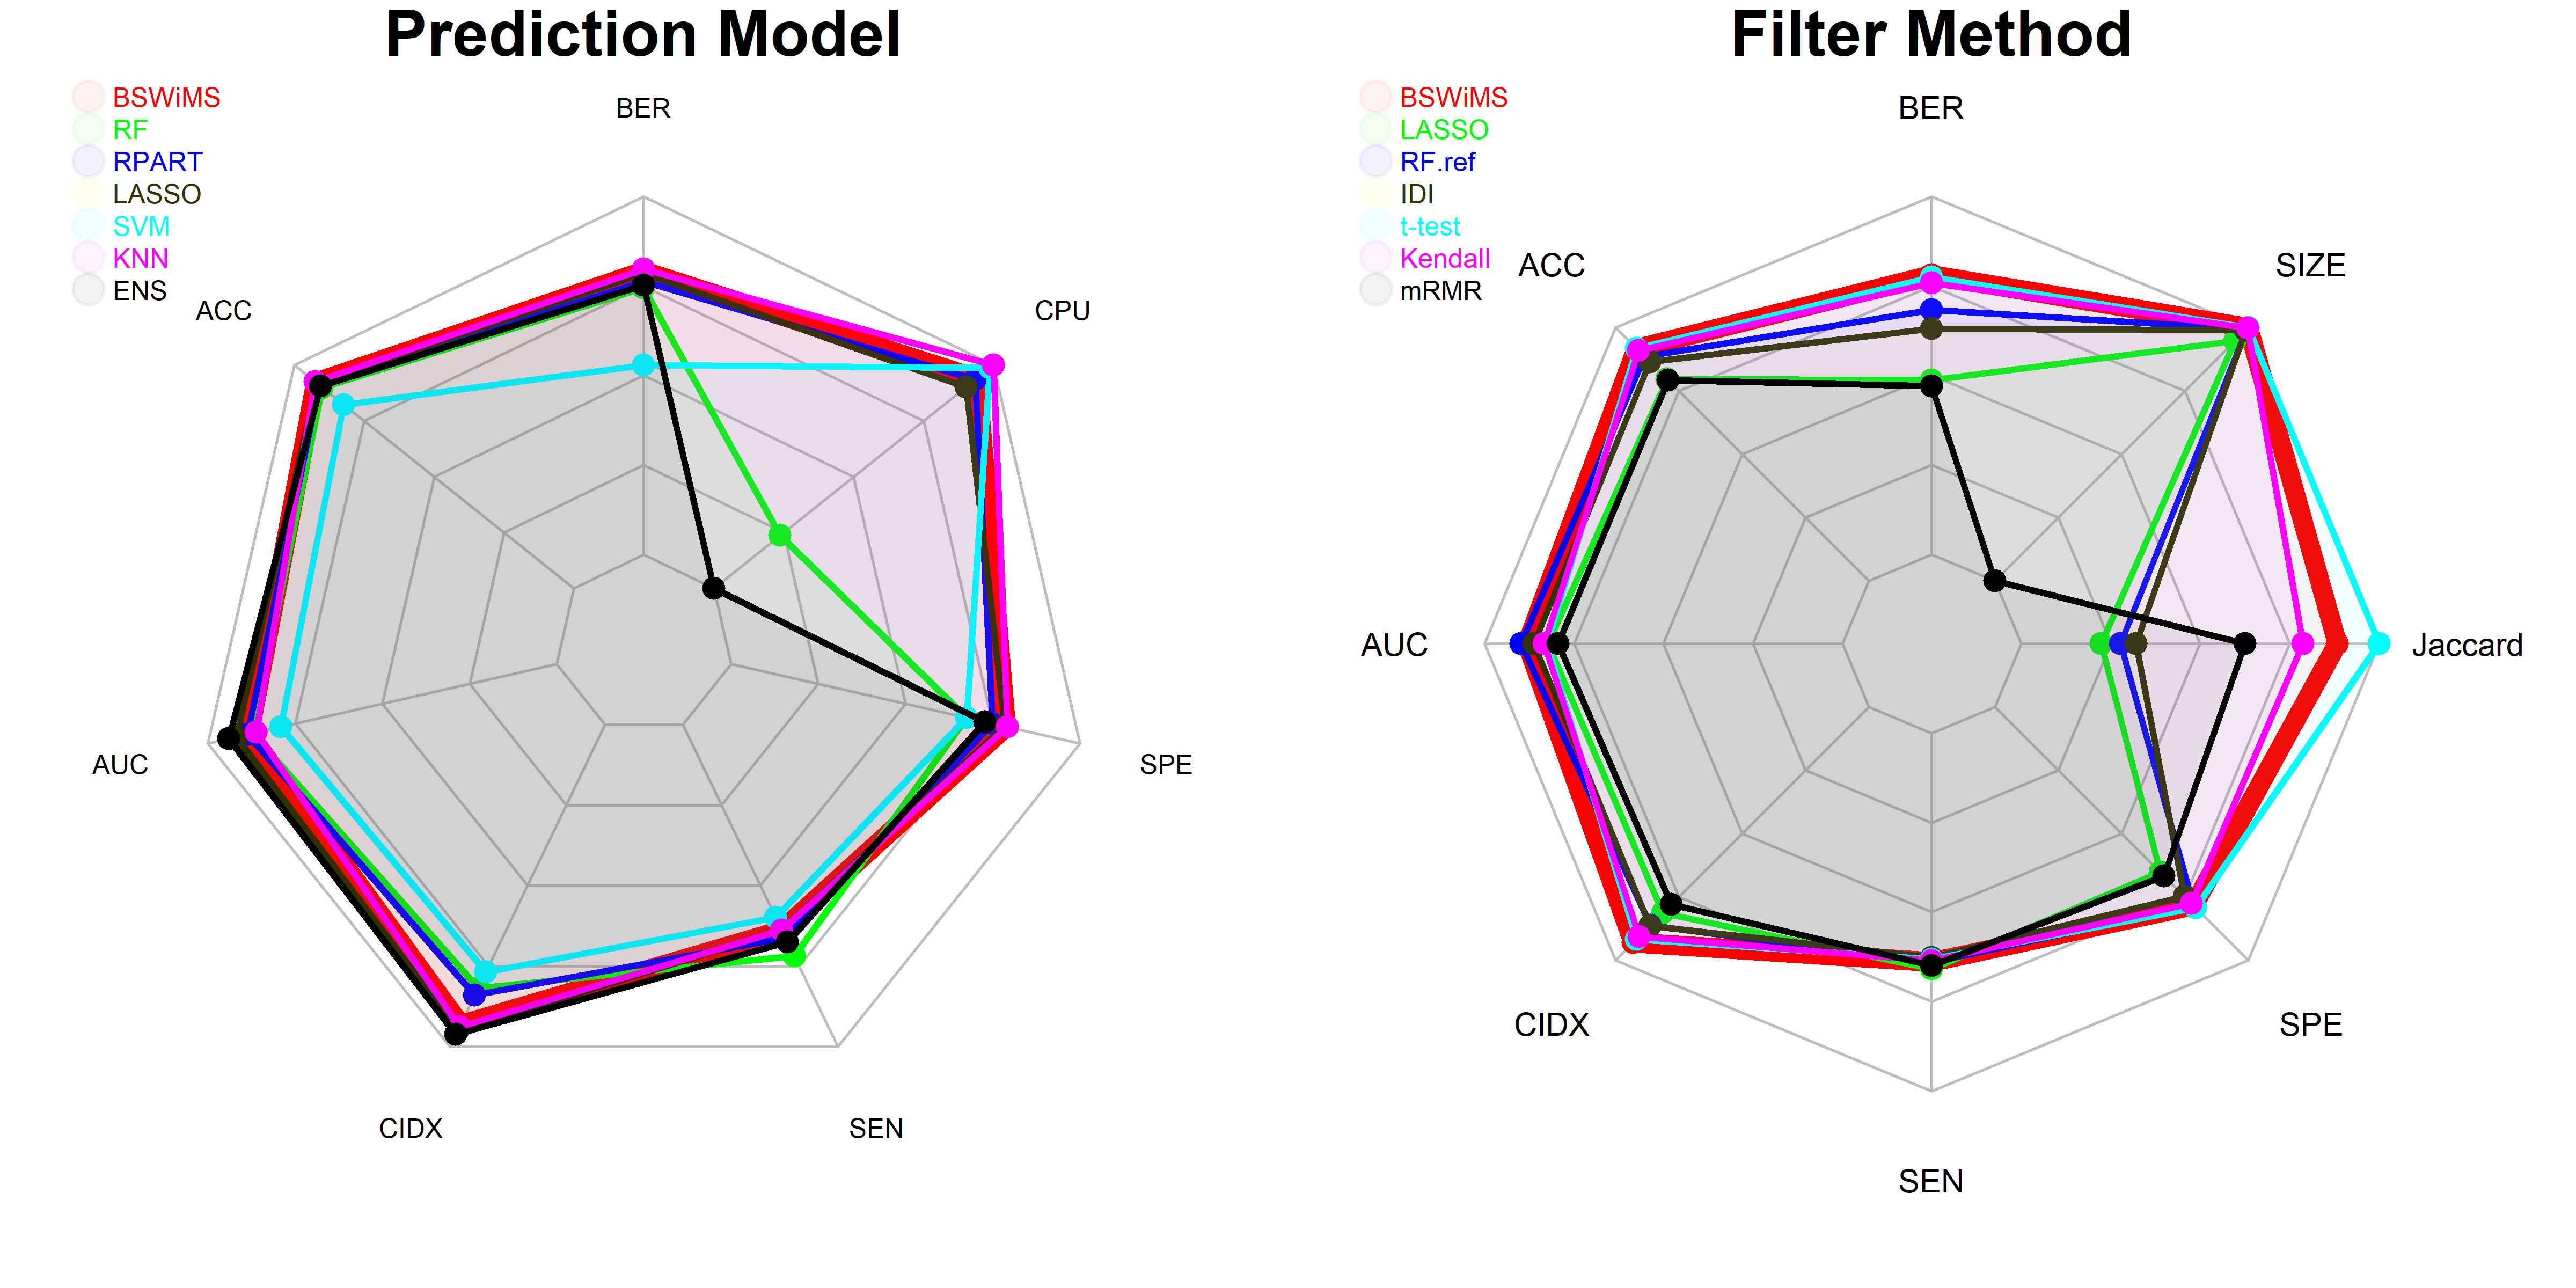
\includegraphics[width=4in]{images/results/fresaRadar.png}}
\caption{{\bf Comparison between the different classifiers and filters of the FRESA.CAD Benchmark } 
Radar plot analysing different metrics to evaluate the performance using different metrics as well as the CPU time between the different classifiers as well as filters of the FRESA.CAD Benchmarking with the complete ADNI dataset for the Cross-validation and using the top 2,500 SNPs as input}
\label{fig19}
\end{figure}

The main goal of the analysis is not only to classify the samples into the two types of diagnosis to better analyze it and treat it, but most importantly to detect precisely which are the given gene variants that could be responsible for the disease as well as to ensure the chosen SNPs have a biological and chemical basis. As such further analysis on the Feature selection process gives insight into those SNPs selected by the different methods as being critical to the decision-making boundary, which enables doctors to precisely genotype only those given genes when a patient comes in and get the results quickly, and also allows researchers to delve into the biochemical reasons of new candidates if found.

The result of one such analysis is shown in Figure 4.18, and shows that there are multiple variants being used by the different methods and they have statistical significance. Definitely the APOE $\epsilon4$(rs429358) marker is being chosen by all the classification methods and this comes as no surprise due to its strong impact on the prediction. RPART is using multiple genes which are not being selected by other methods, and LASSO is using more SNPs but which are also being selected by the other methods. Both of these approaches are giving good results in the classification. mRMR is selecting all of the most frequent markers, but as seen before this does not mean it will perform better. Interesting candidates for further analysis could be rs67636621, rs76566842 and rs16905109 based on this figure.

\begin{figure}[!ht]
\centerline{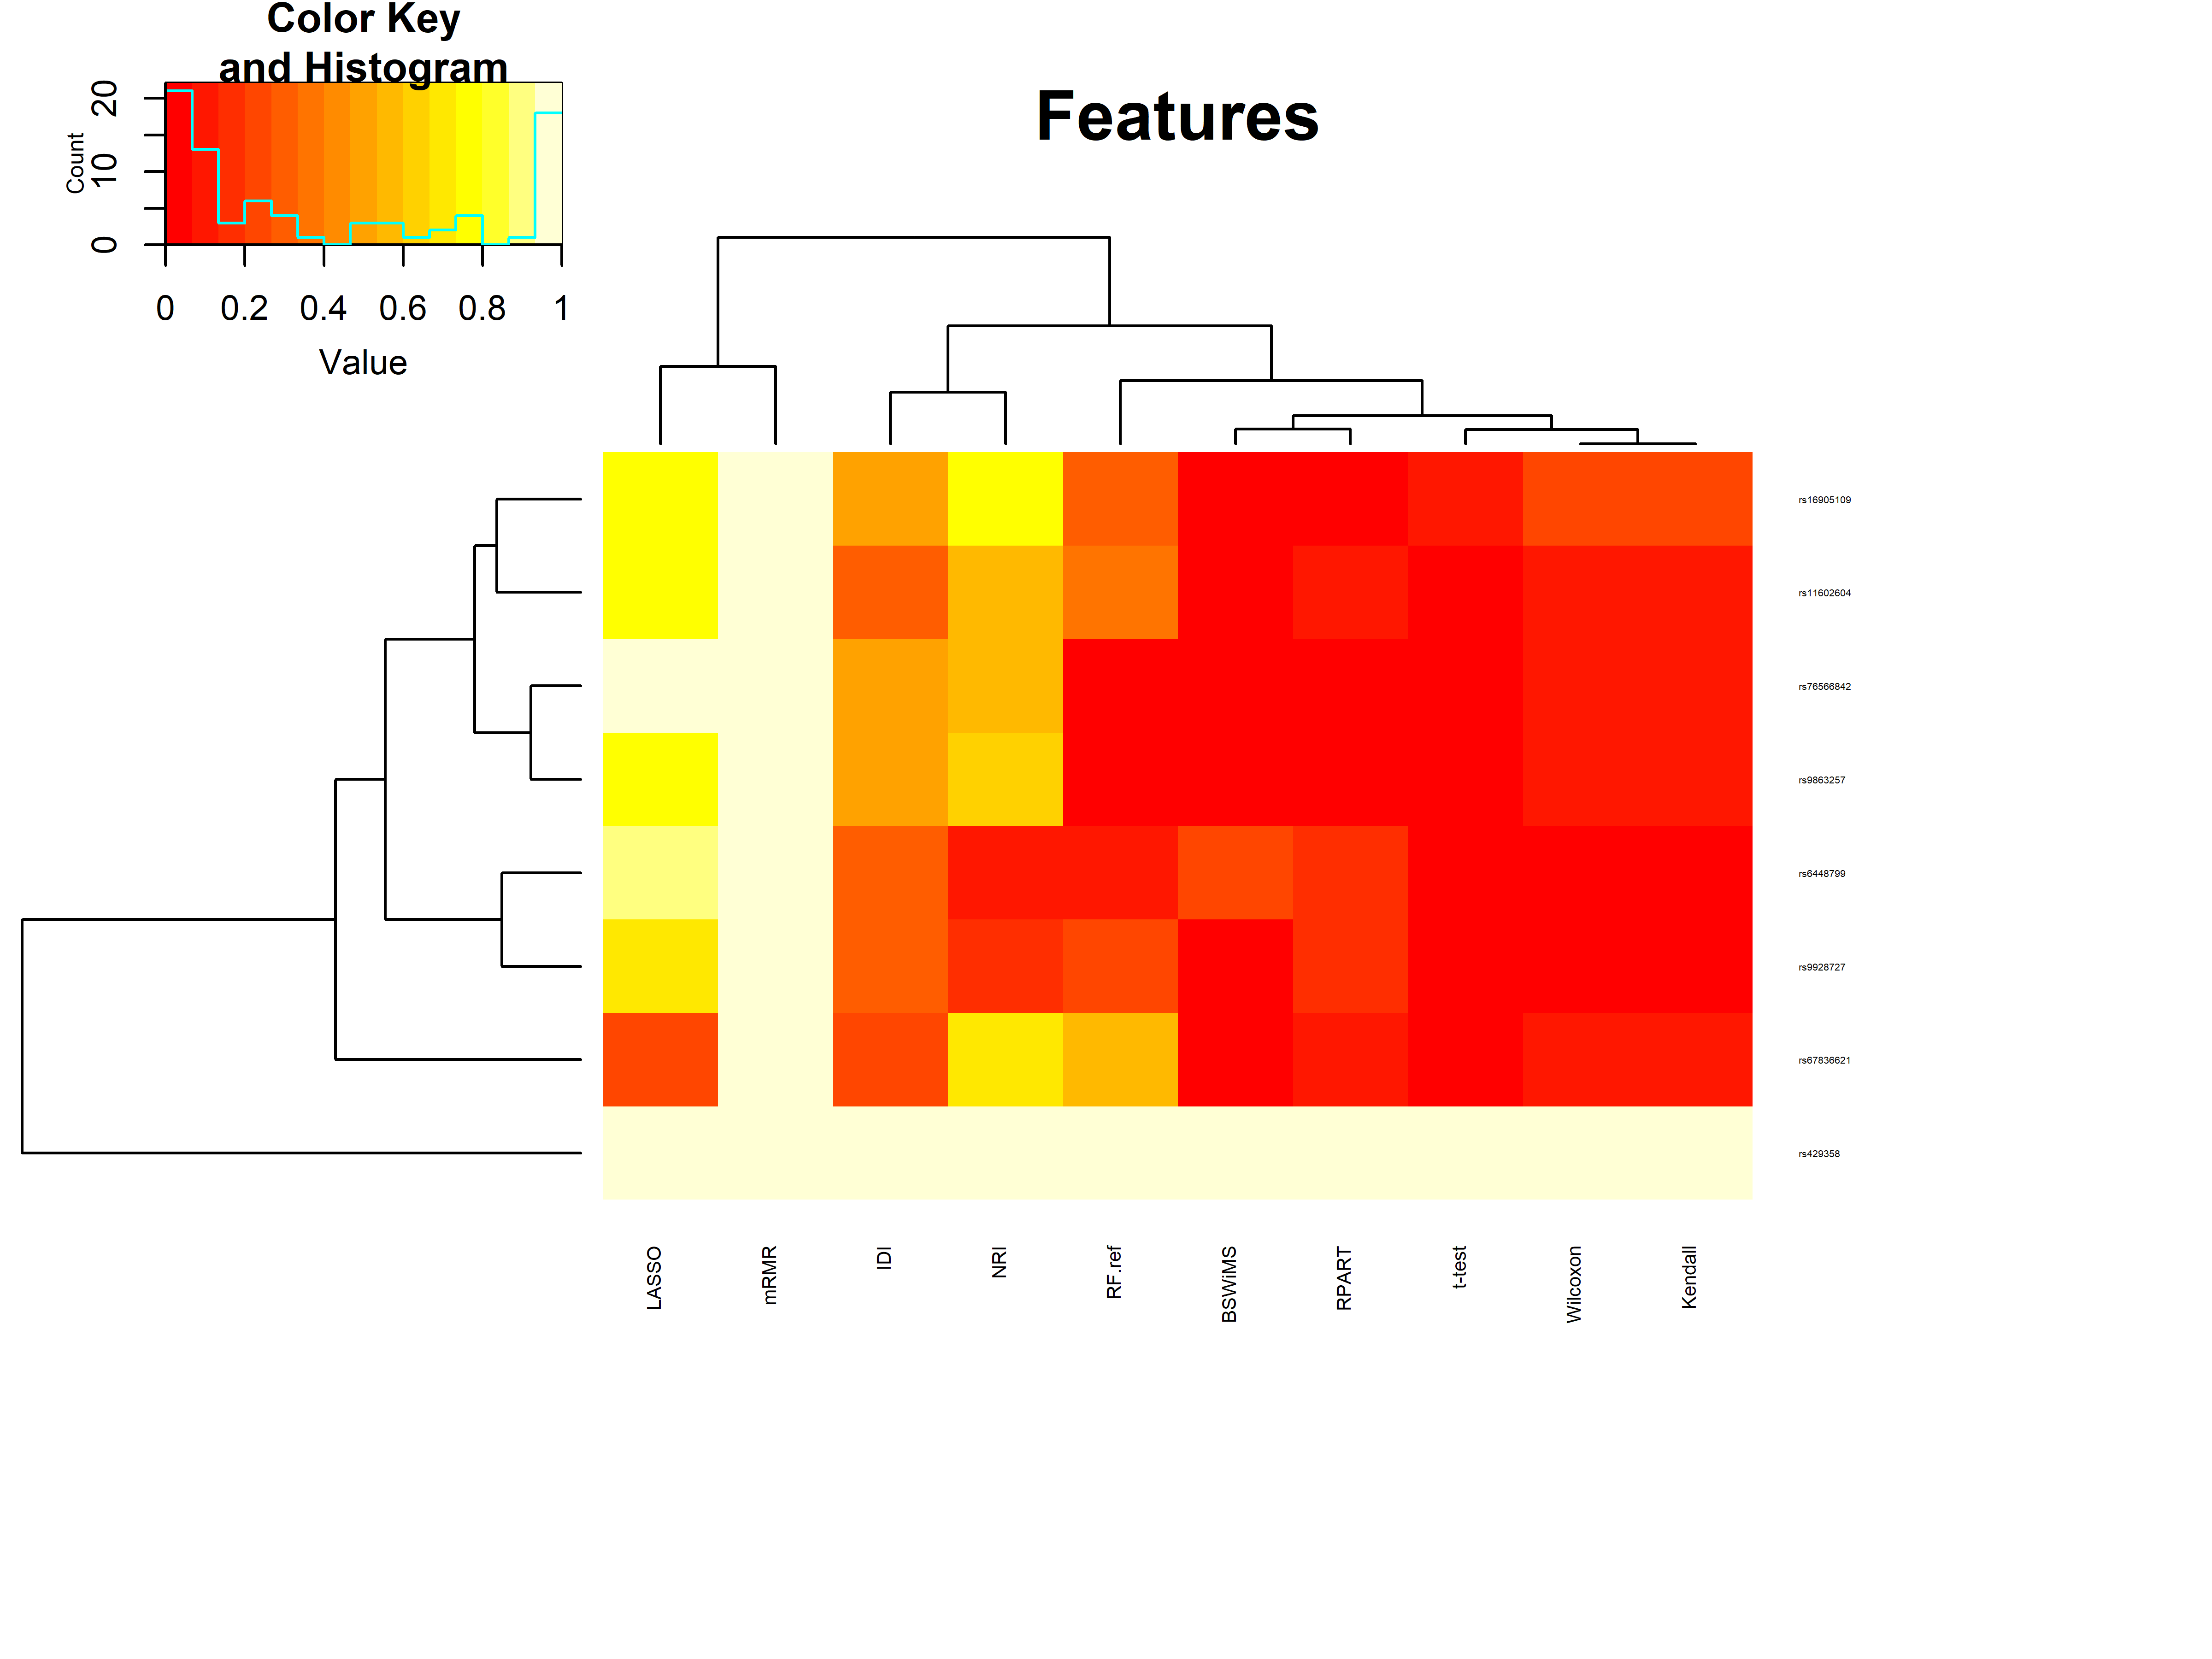
\includegraphics[width=4in]{images/results/fresaSNPs.png}}
\caption{{\bf SNPs chosen more than 10\% of the time as features of the FRESA.CAD Benchmark} 
Heatmap of the main SNPs being chosen across all the classifiers. The Y axis are the main SNPs being selected while the X axis represents the different classifiers of the FRESA.CAD Benchmarking with the complete ADNI dataset for the Cross-validation and using the top 2,500 SNPs as input}
\label{fig20}
\end{figure}
 
 
To further analyze the top candidates Table 1 contains the results of the 8 most important SNPs that are found (The only ones selected by more than 10\% of the models. Most of them have a quite high significance according to the Wilcoxon test when doing Univariate Analysis. The APOE $\epsilon4$ gene definitely gives a very strong predictive power, and the remaining genes are then used to further improve the model. One note: The ROC AUC value per SNP is not directly comparable to previous ROC AUC values shown before due to the calculation procedure, as it will be further shown in the next analysis. Also, while some have a better Wilcoxon result that does not necessarily relate to a higher classification power or vice-versa, as it happens with rs11602604. The results seem to prove the current knowledge that APOE $\epsilon4$ is the main factor with other SNPs complementing with small effects, thus it makes sense that models always select it. And to complement it as the other results also show how the models with more SNPs slightly outperform the smaller models

\begin{table}[ht!]
    \begin{center}
        \begin{tabular}{|c|c|c|c|}
        \hline
        \textbf{SNP}   &  \textbf{ROC AUC} &  \textbf{WILCOX} &  \textbf{FREQ} \\ \hline
rs429358   &	0.6961 &	0       &	1.000 \\ \hline
rs67836621  &	0.5815 &	8e-04   &	0.298 \\ \hline
rs9928727	&	0.5787 &	9e-04   &	0.269 \\ \hline
rs11602604	&	0.5783 &	3e-04   &	0.321 \\ \hline
rs6448799	&	0.5751 &	6e-04   &	0.288 \\ \hline
rs16905109	&	0.5484 &	0.0011  &	0.383 \\ \hline
rs76566842	&	0.534  &	0.1619  &	0.327 \\ \hline
rs9863257	&	0.5321 &	0.1955  &	0.323 \\ \hline
        \end{tabular}
    \end{center}
  \caption{Top SNPs selected as important features for the full ADNI Dataset}
  \label{topsnps}
\end{table}

\newpage
The second analysis to perform is on the reduced validation dataset without samples from the IGAP using the top 1,000 SNPs. As before, this has the problem of being a small sample size. Contrasting the previous results are the ROC Curves from this dataset as shown in Figure 4.19 and Figure 4.20. The results are much lower, in the order of 0.50\~0.60. In this case only BSWiMS, RPART and the Ensemble give useful predictions. This shows again the complexity of the given problem with a small, unbalanced dataset for validation due to independent from the statistical analysis and reinforces the results from previous analysis.

 \begin{figure}[!ht]
\centerline{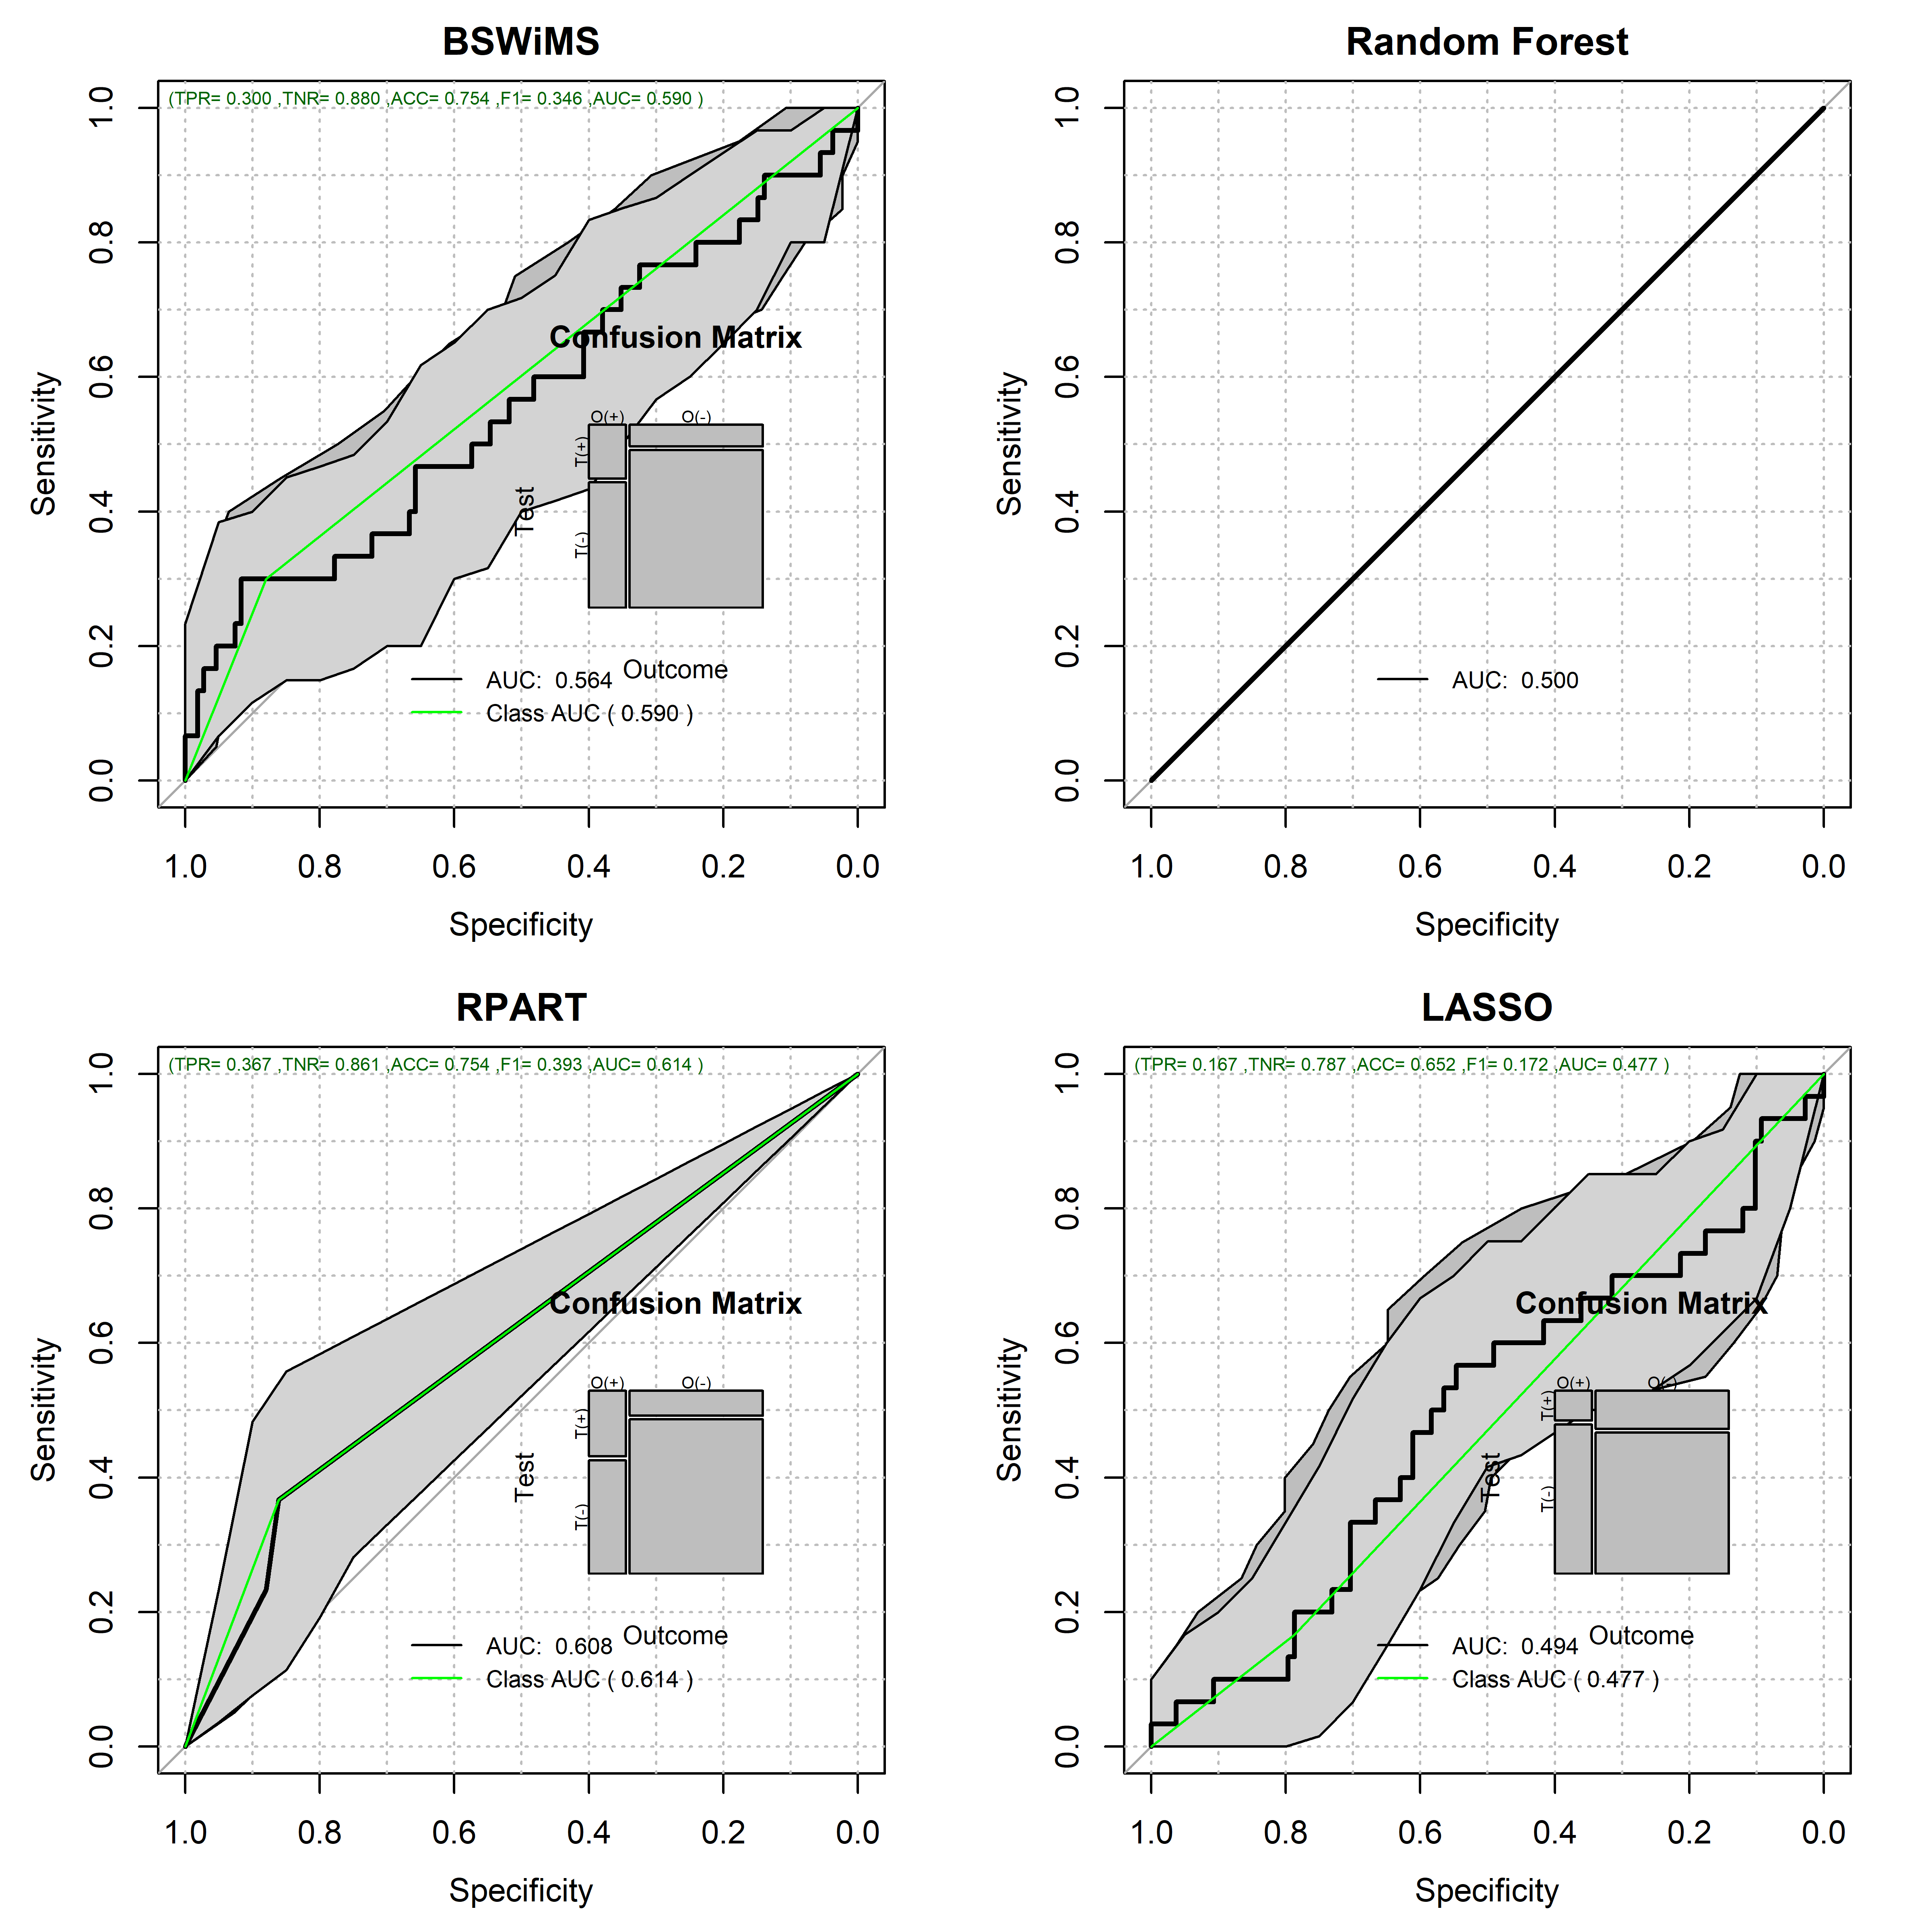
\includegraphics[width=3in]{images/results/fresaCurves1Val.png}}
\caption{{\bf Validation ROC Curves for the FRESA.CAD Benchmarking Classifiers} 
ROC Curves obtained using BSWiMS, Random Forest, RPART and LASSO of the FRESA.CAD Benchmarking with the validation dataset for the Cross-validation and using the top 1,000 SNPs as input}
\label{fig24}
\end{figure}

 \begin{figure}[!ht]
\centerline{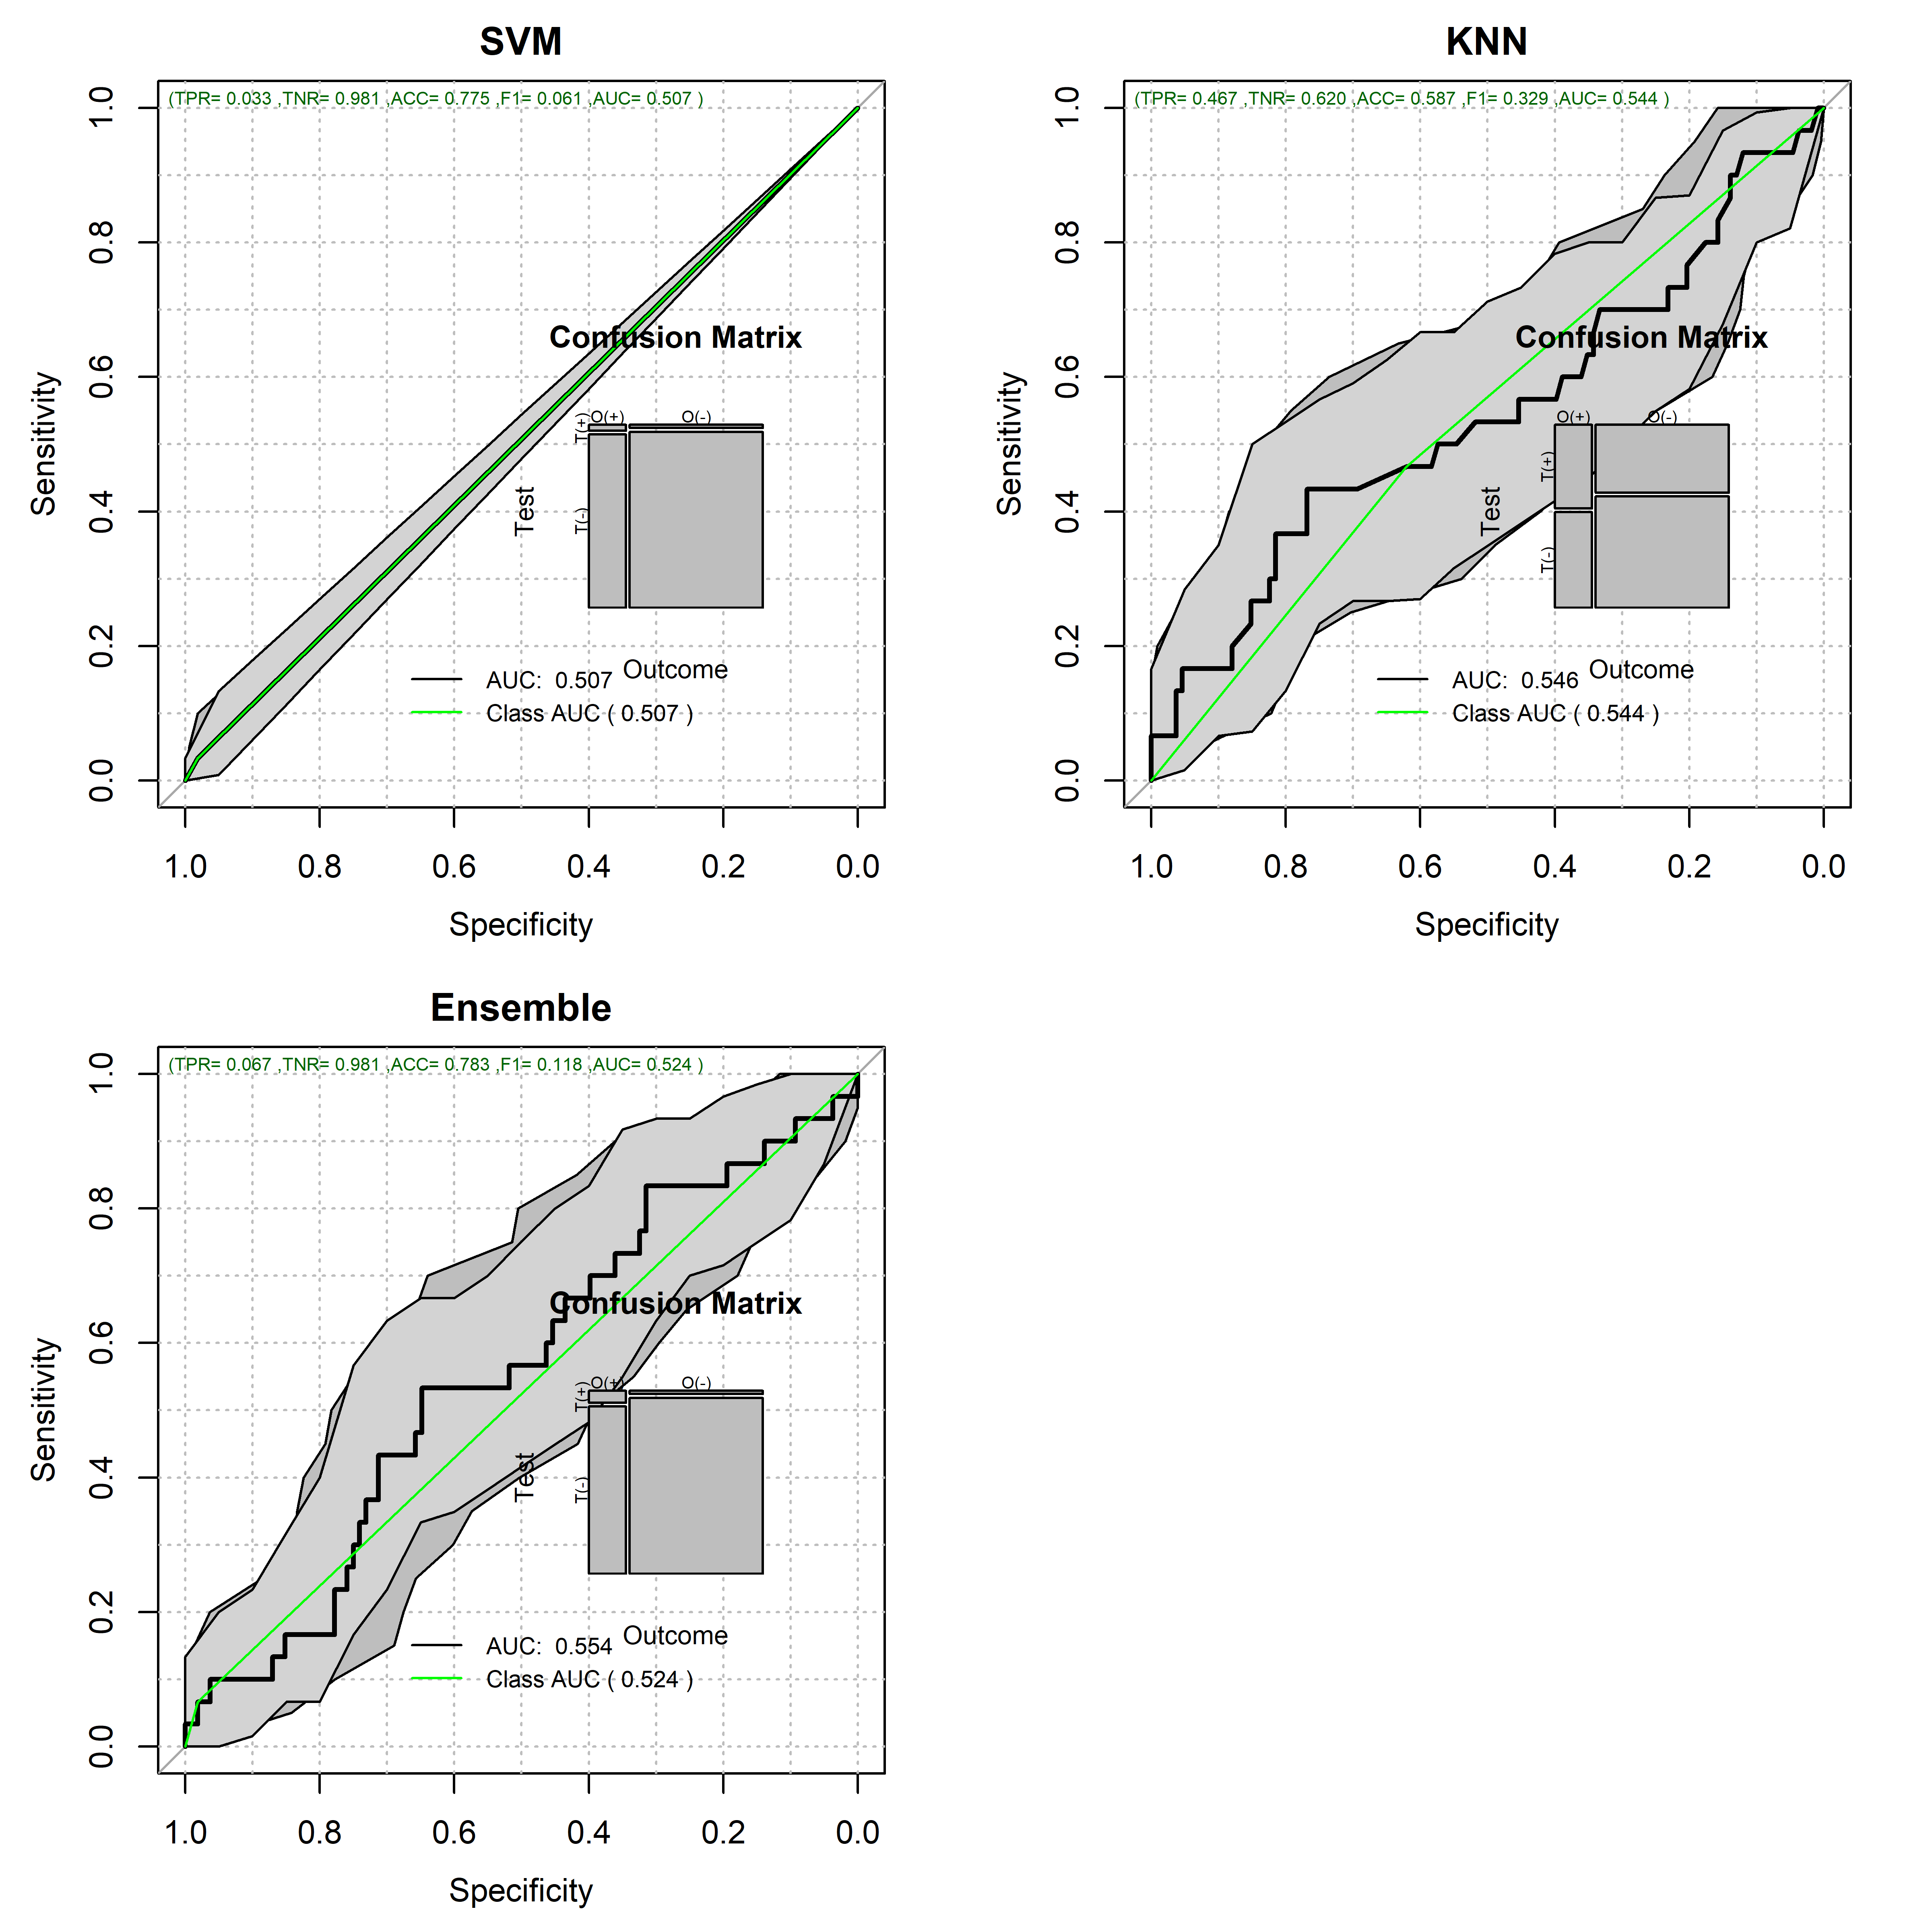
\includegraphics[width=3in]{images/results/fresaCurves2Val.png}}
\caption{{\bf Validation ROC Curves for the FRESA.CAD Benchmarking Classifiers (Continued)} 
ROC Curves obtained using SVM, KNN and the Ensemble of the FRESA.CAD Benchmarking with the validation dataset for the Cross-validation and using the top 1,000 SNPs as inputs}
\label{fig25}
\end{figure}

Figure 4.21 and 4.22 reinforce this by showing the different metrics. As seen the accuracy tends to be quite high, but this is due to the class unbalance. Thus the Balanced error and the ROC give better metrics.  BSWiMS and RPART are shown to have the lowest Balanced Error and the best ROC AUC scores, followed by the Ensemble. Thus for this sub problem either model would be better than the Ensemble in contrast to the previous Analysis. An important detail to notice is the larger confidence intervals, as the dataset has a lower number of features this confidence interval is higher and as such it could be possible that all models perform quite equally when tested outside outside of this dataset. The same happens with the filter combinations, where it can be seen that there is no clear filter better than the rest with certainty, although Naive Bayes tends to show better results than the others.

 \begin{figure}[!ht]
\centerline{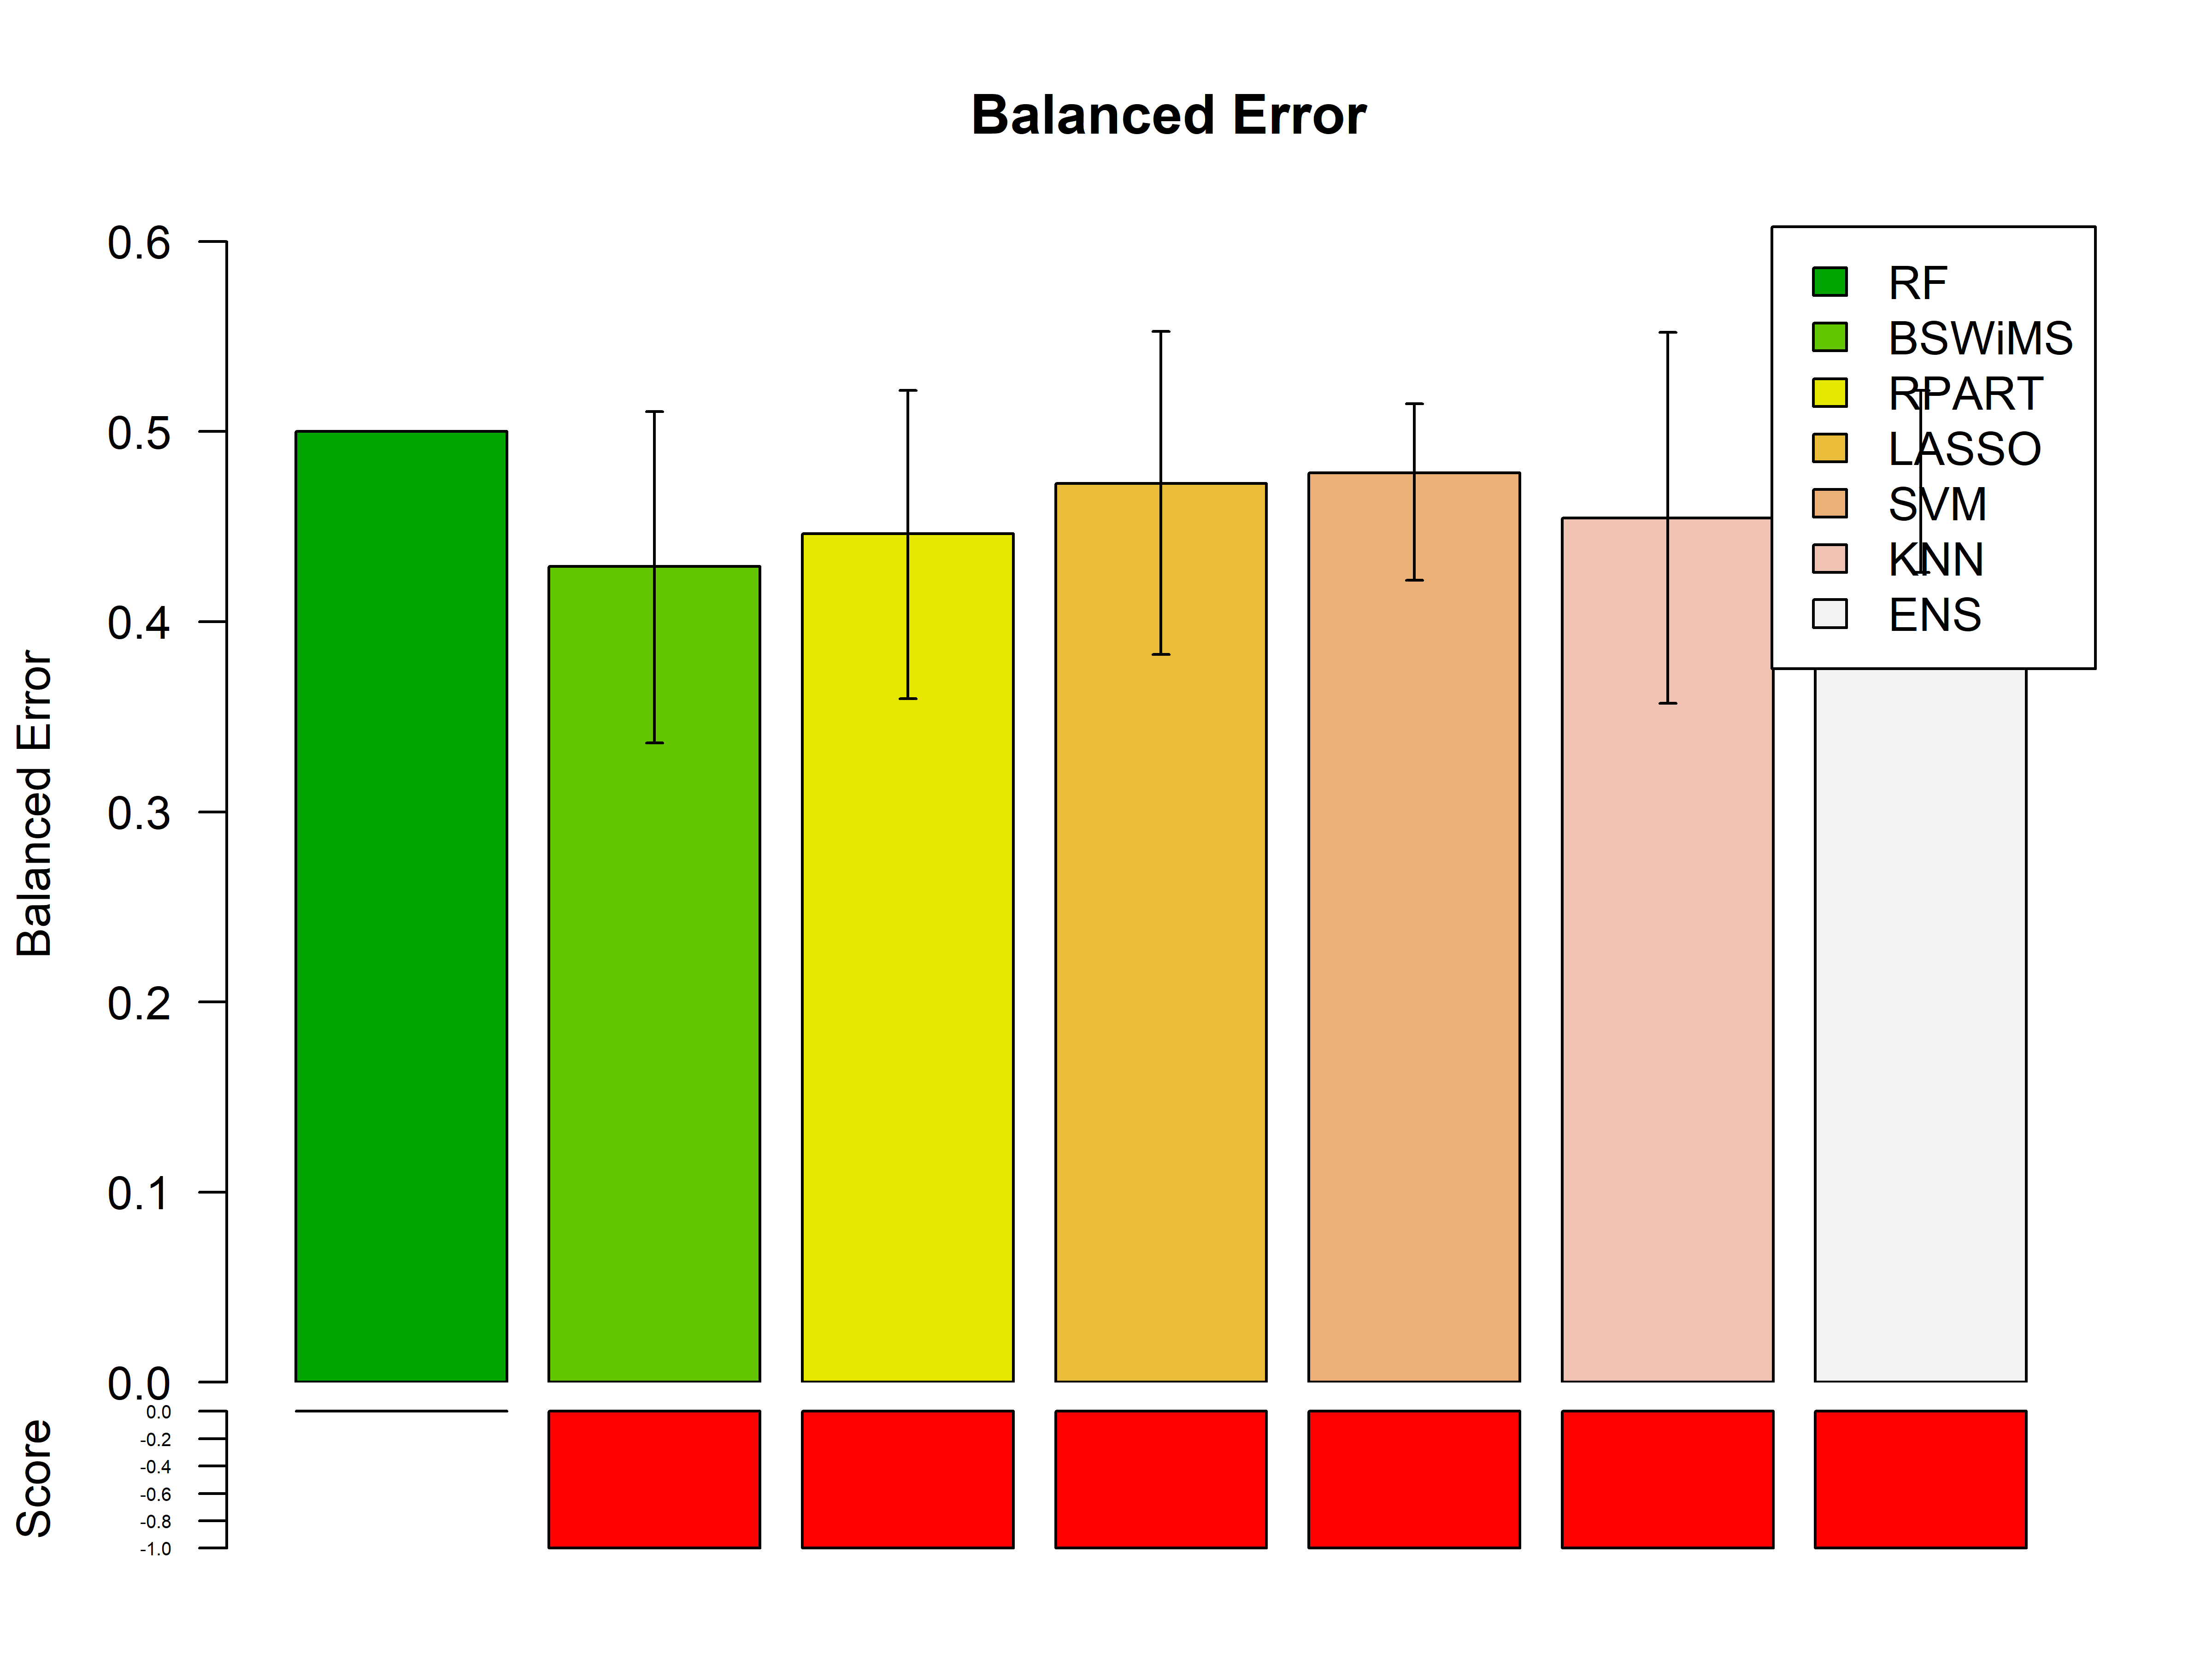
\includegraphics[width=5in,height=2in]{images/results/fresaBEVal.png}}
\centerline{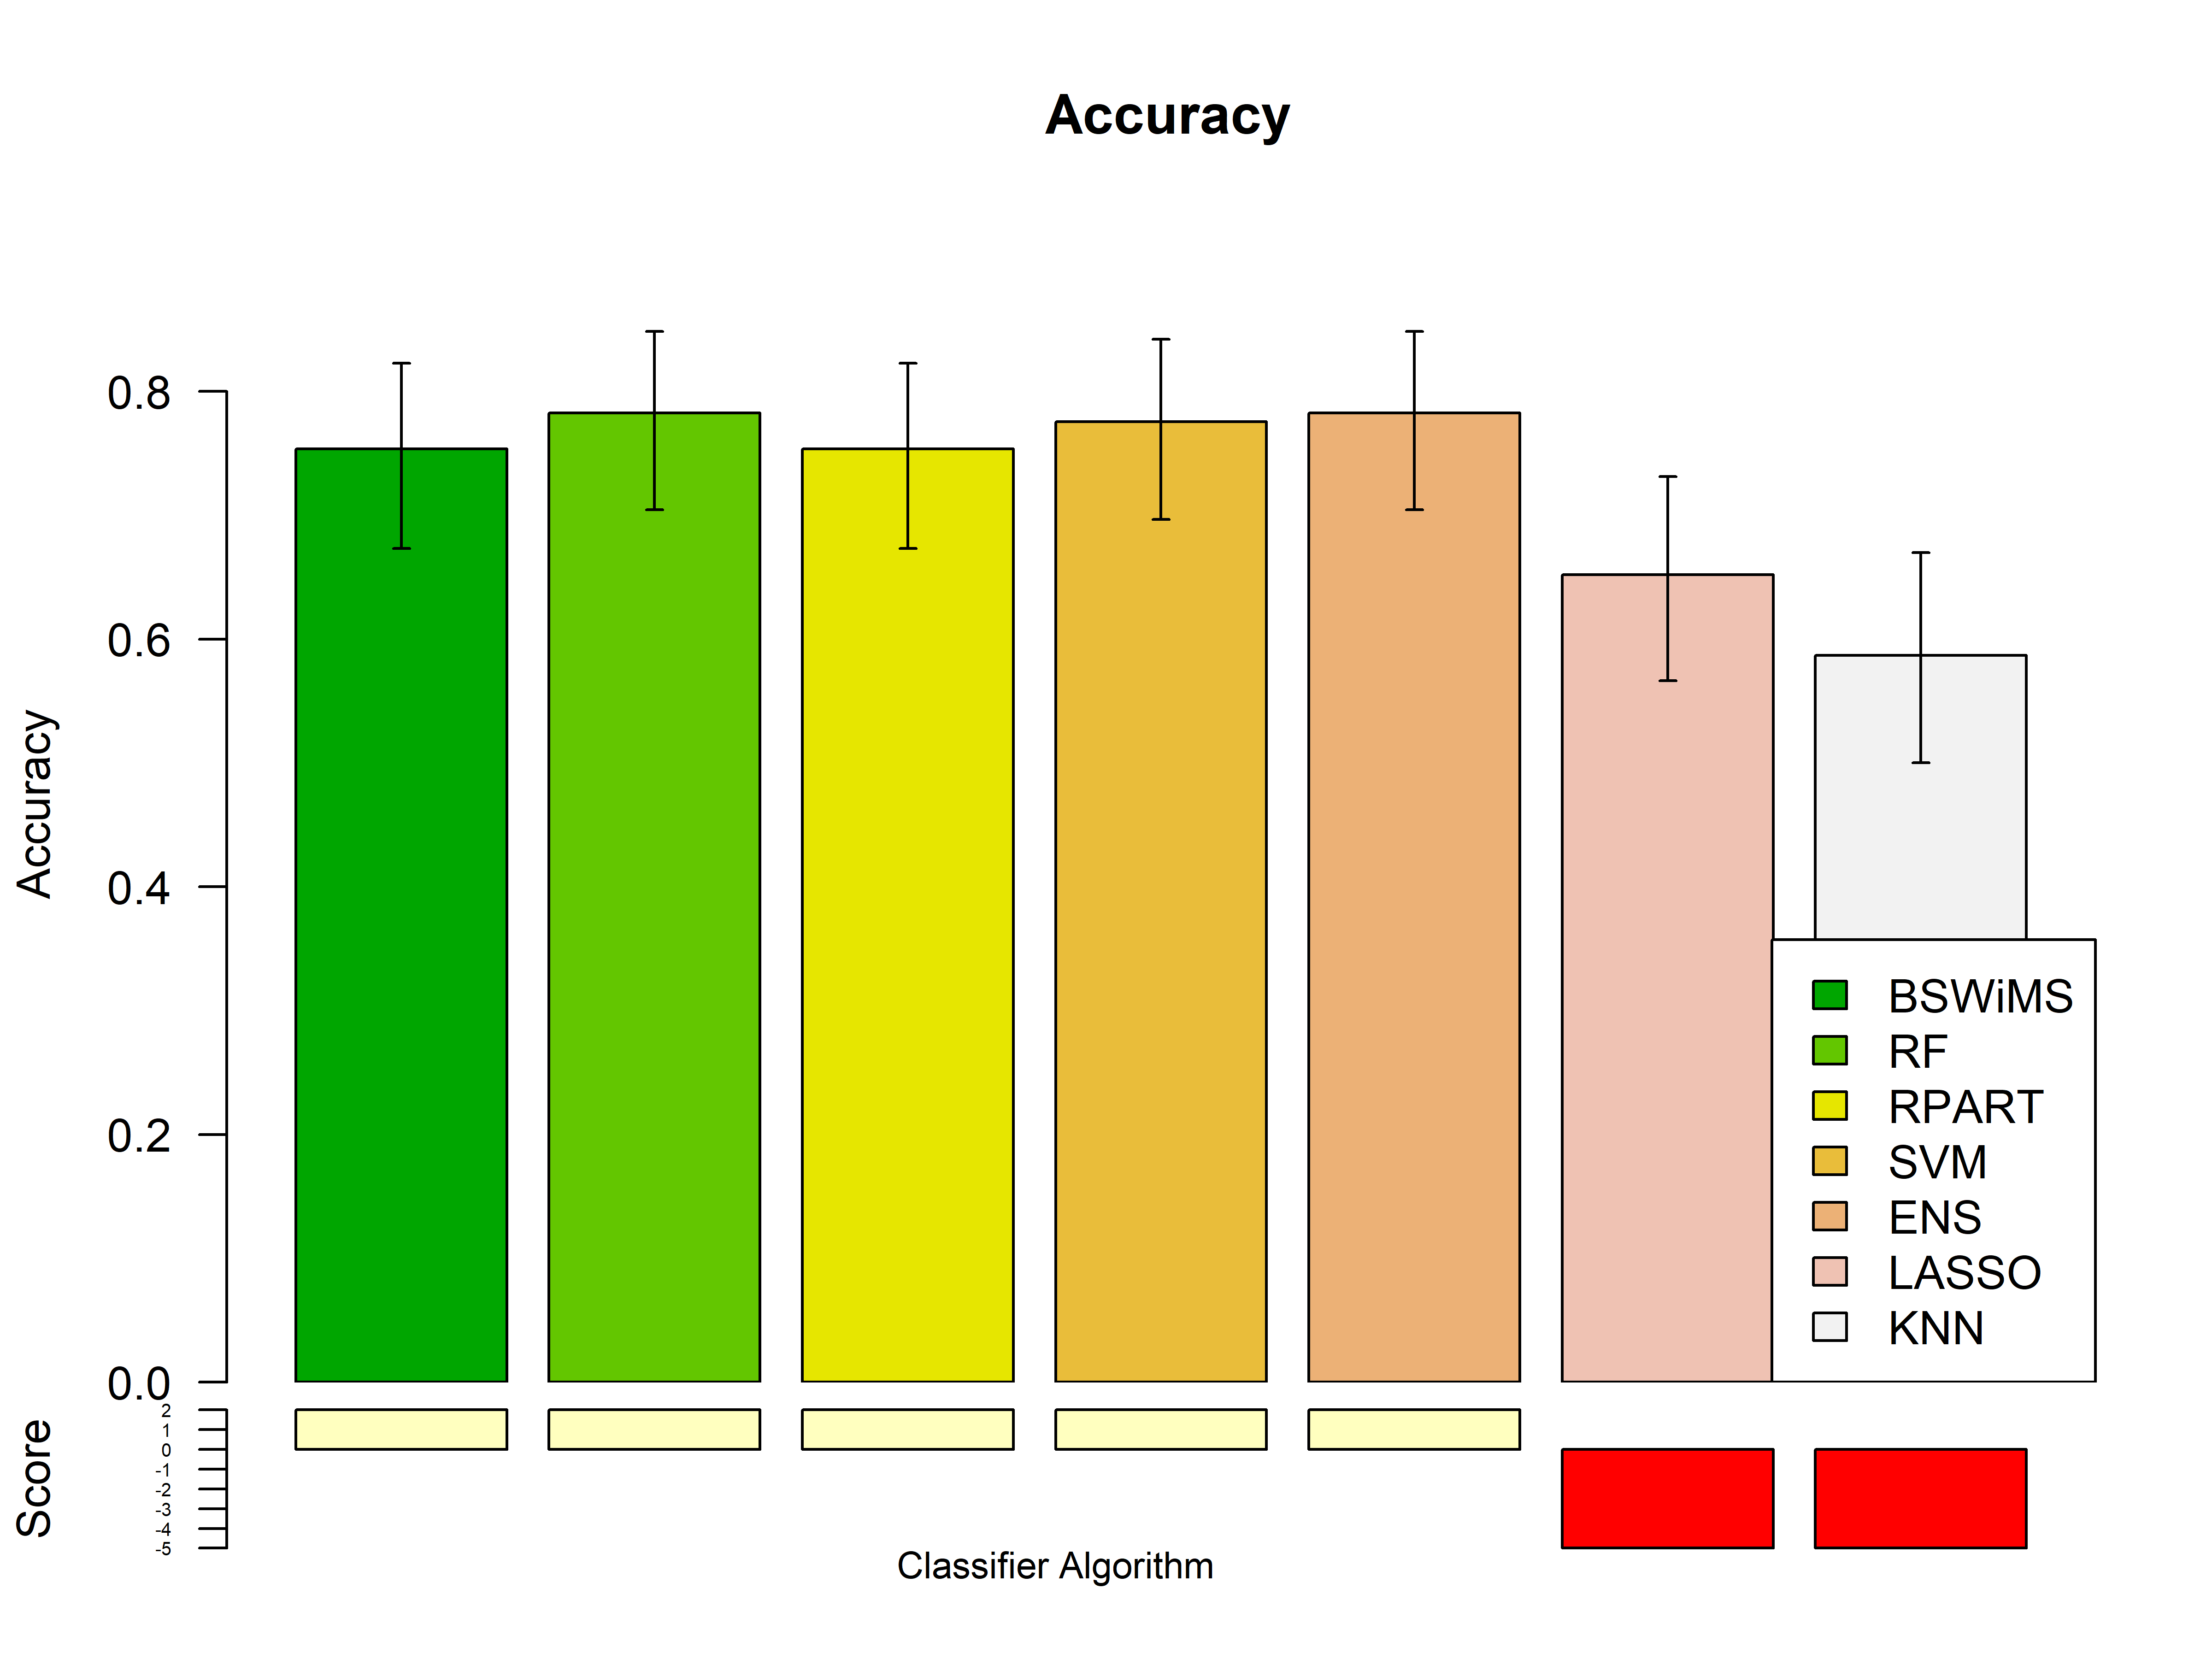
\includegraphics[width=5in,height=2in]{images/results/fresaAccVal.png}}
\centerline{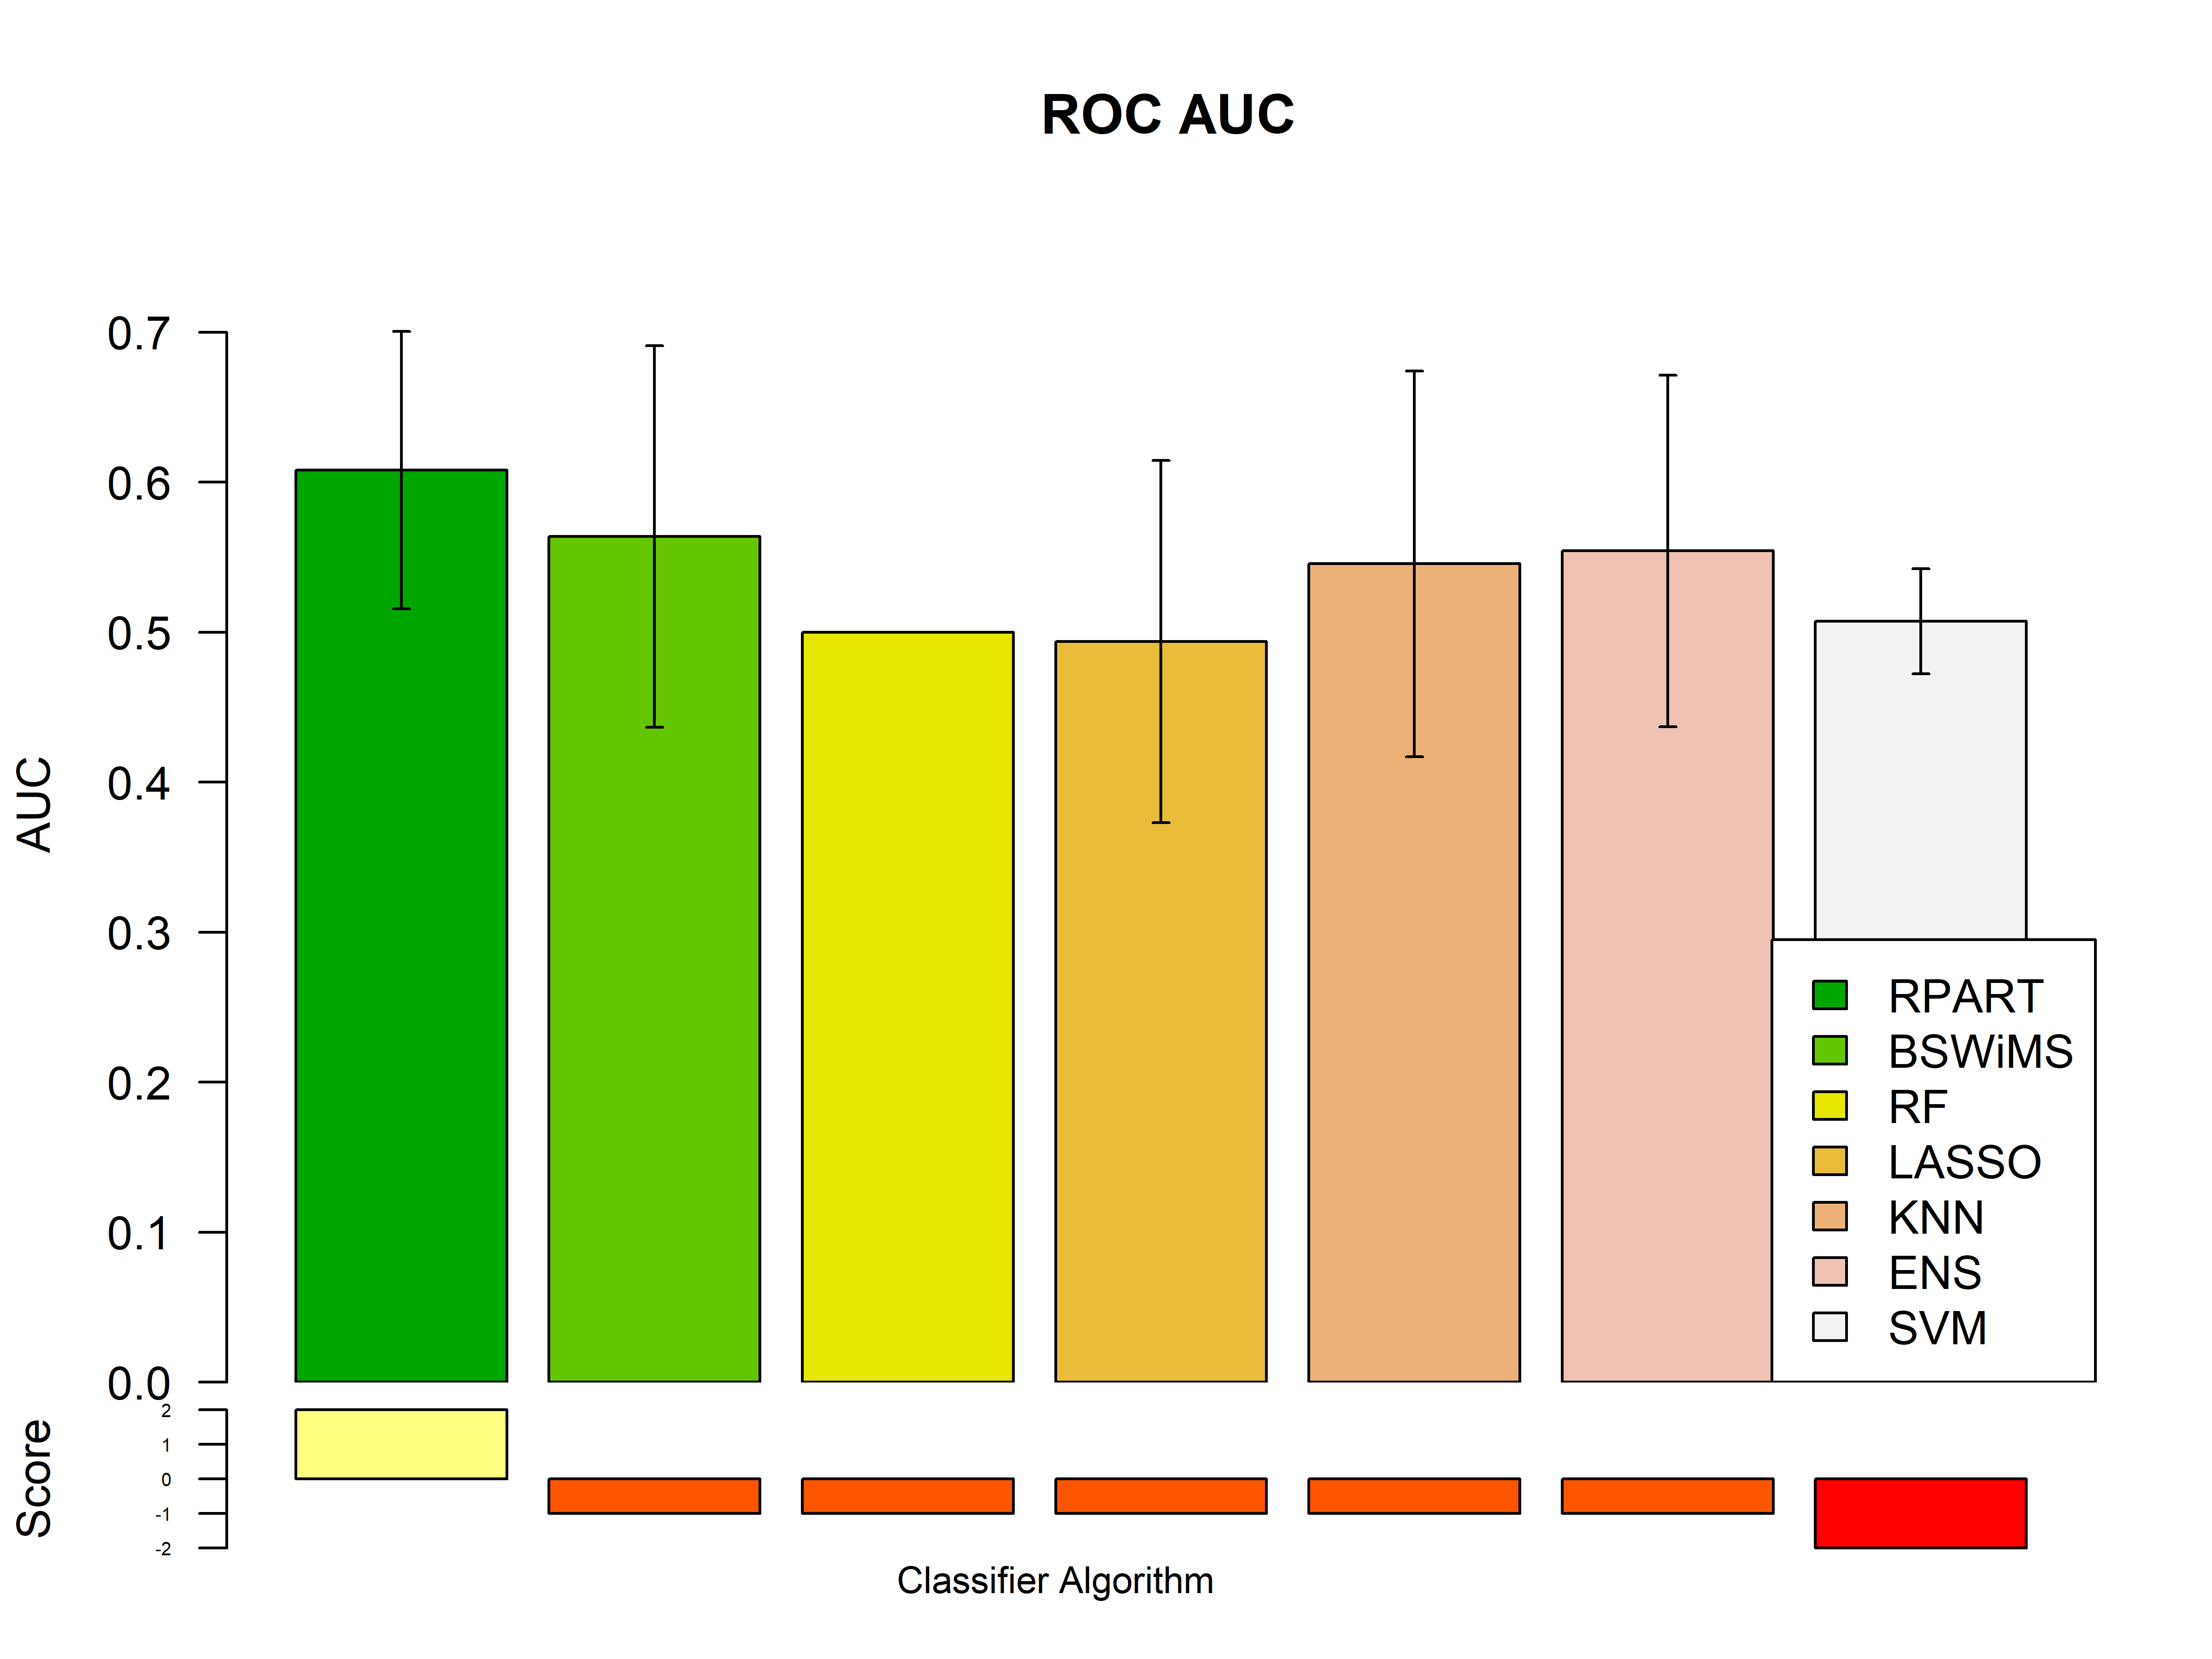
\includegraphics[width=5in,height=2in]{images/results/fresaAUCVal.png}}
\caption{{\bf Validation Balanced Error, Accuracy and AUC of the FRESA.CAD Benchmark classifiers} 
Comparison between the Balanced Error, Accuracy and AUC Score obtained using the different classification methods of the FRESA.CAD Benchmarking with the validation dataset for the Cross-validation and using the top 1,000 SNPs as input}
\label{fig26}
\end{figure}

   
\begin{figure}[!ht]
\centerline{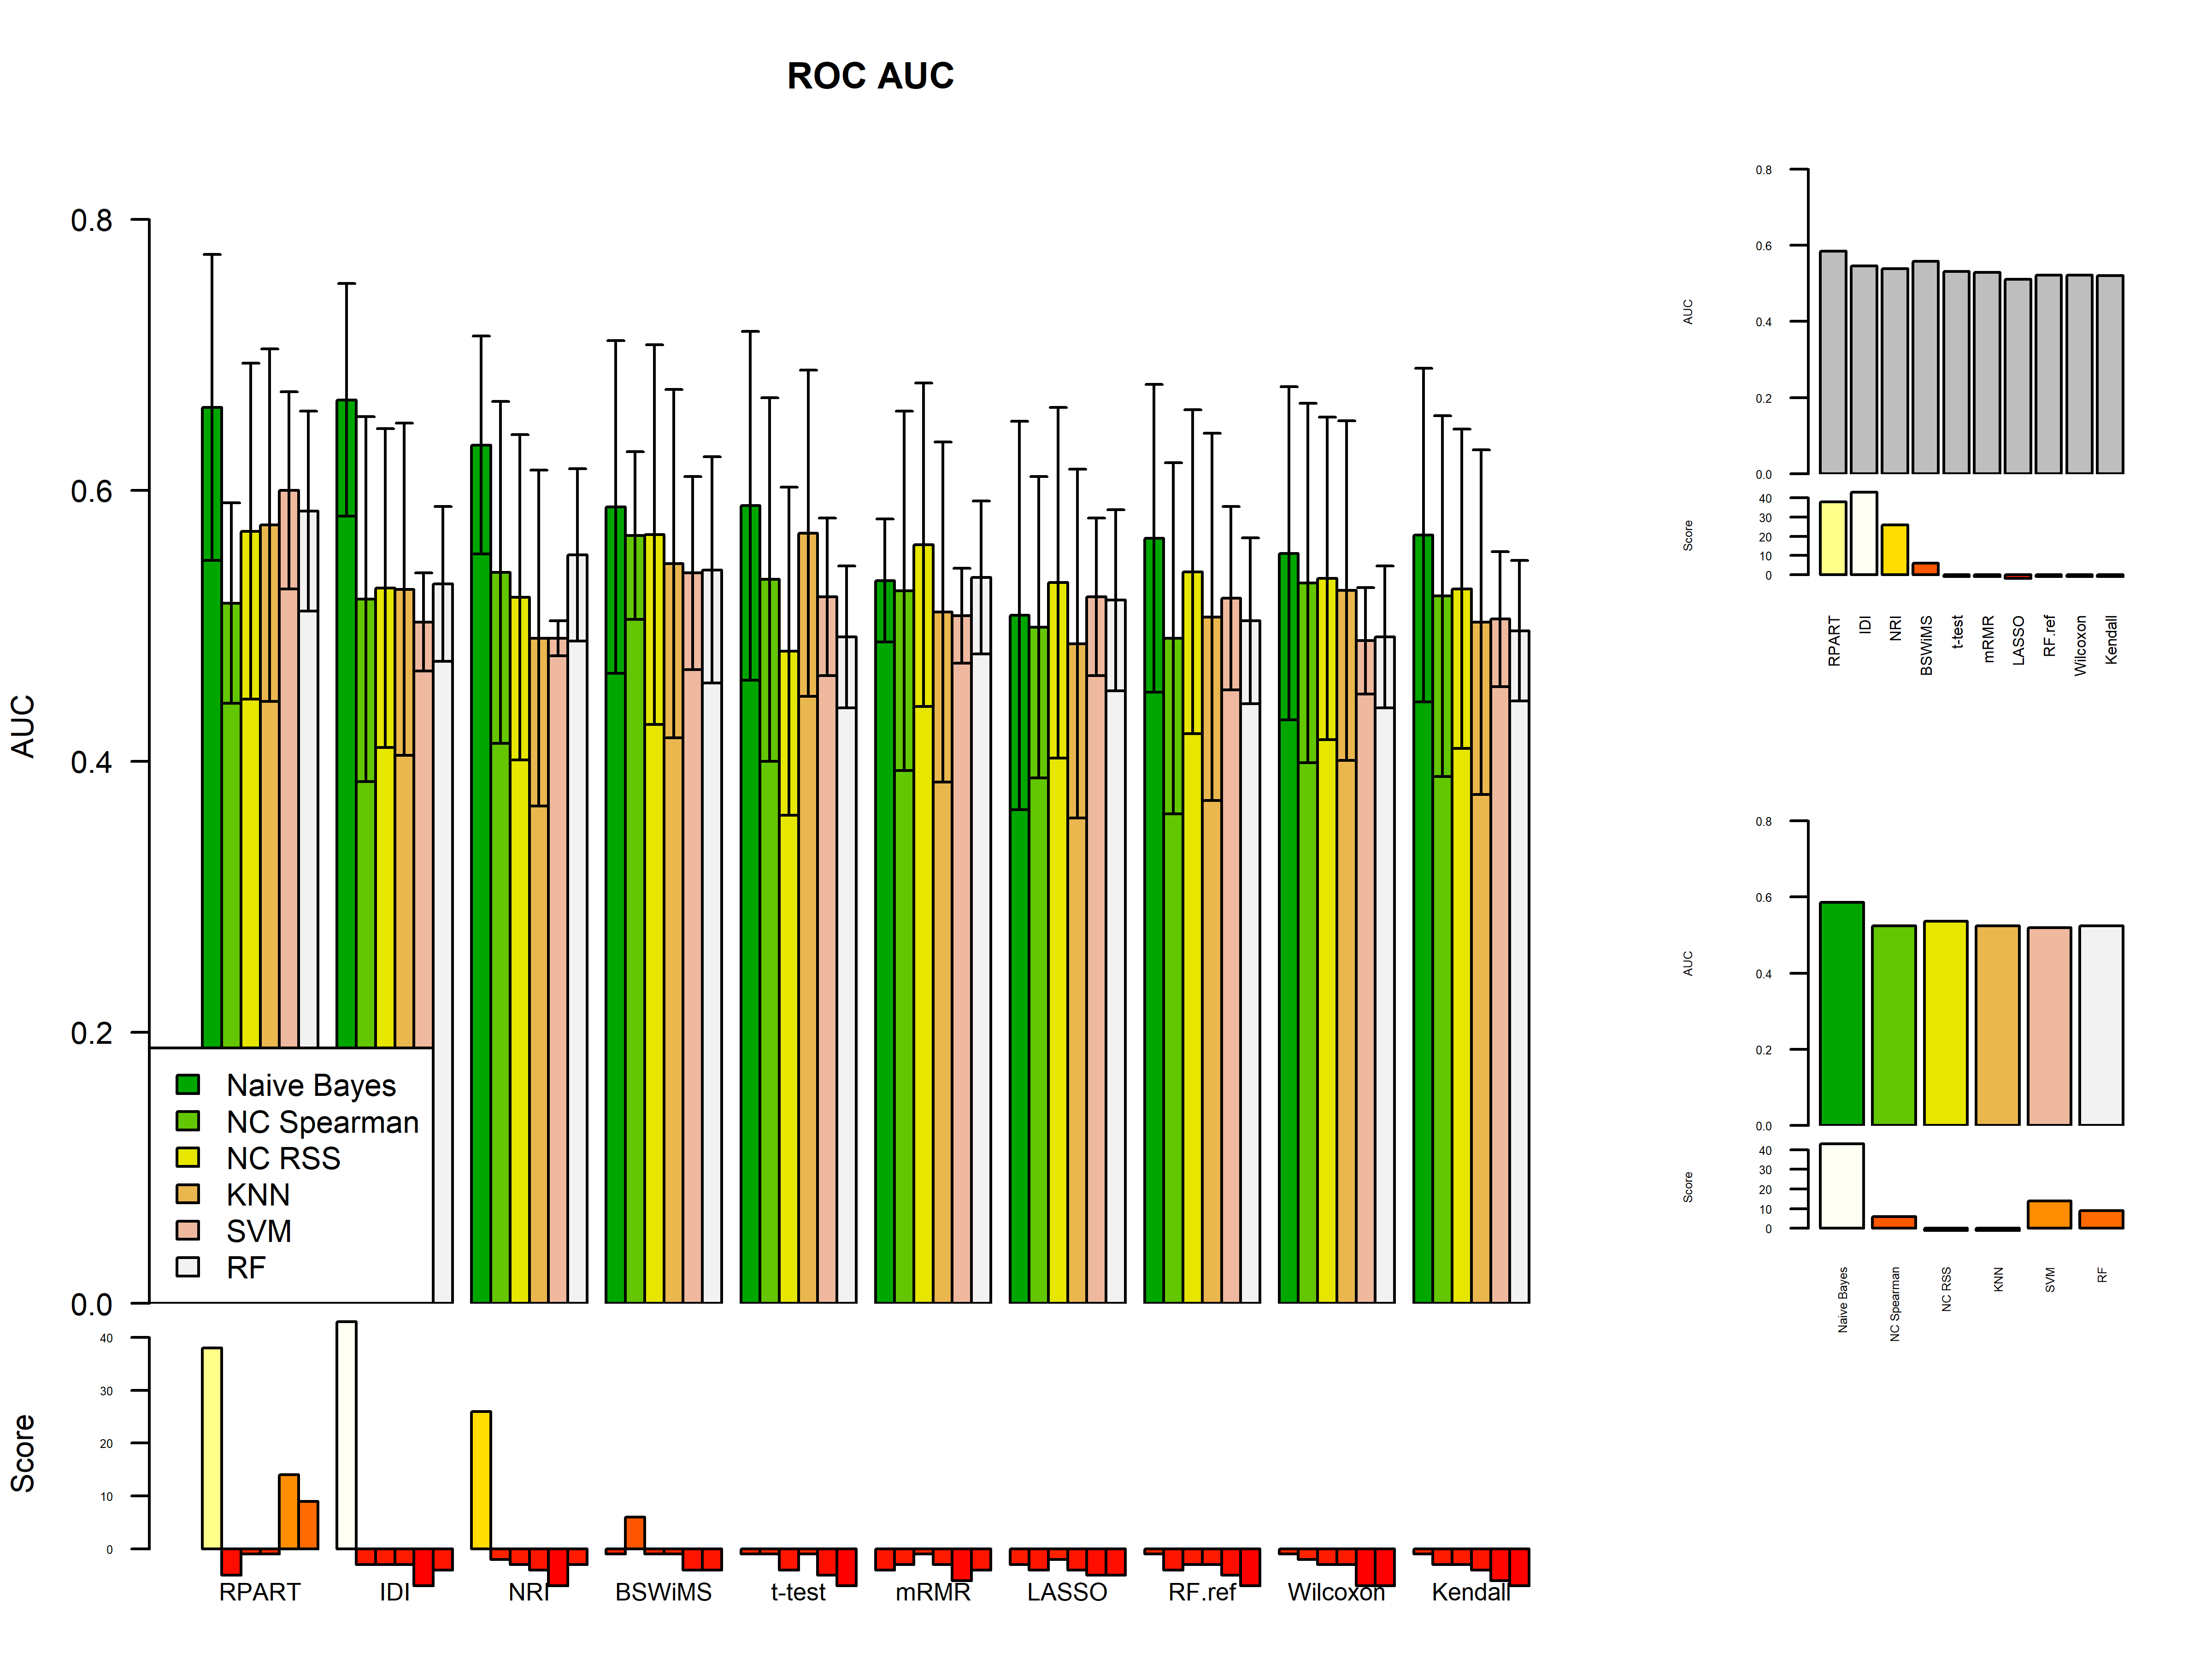
\includegraphics[width=5in,height=2in]{images/results/fresaConcVal.png}}
\centerline{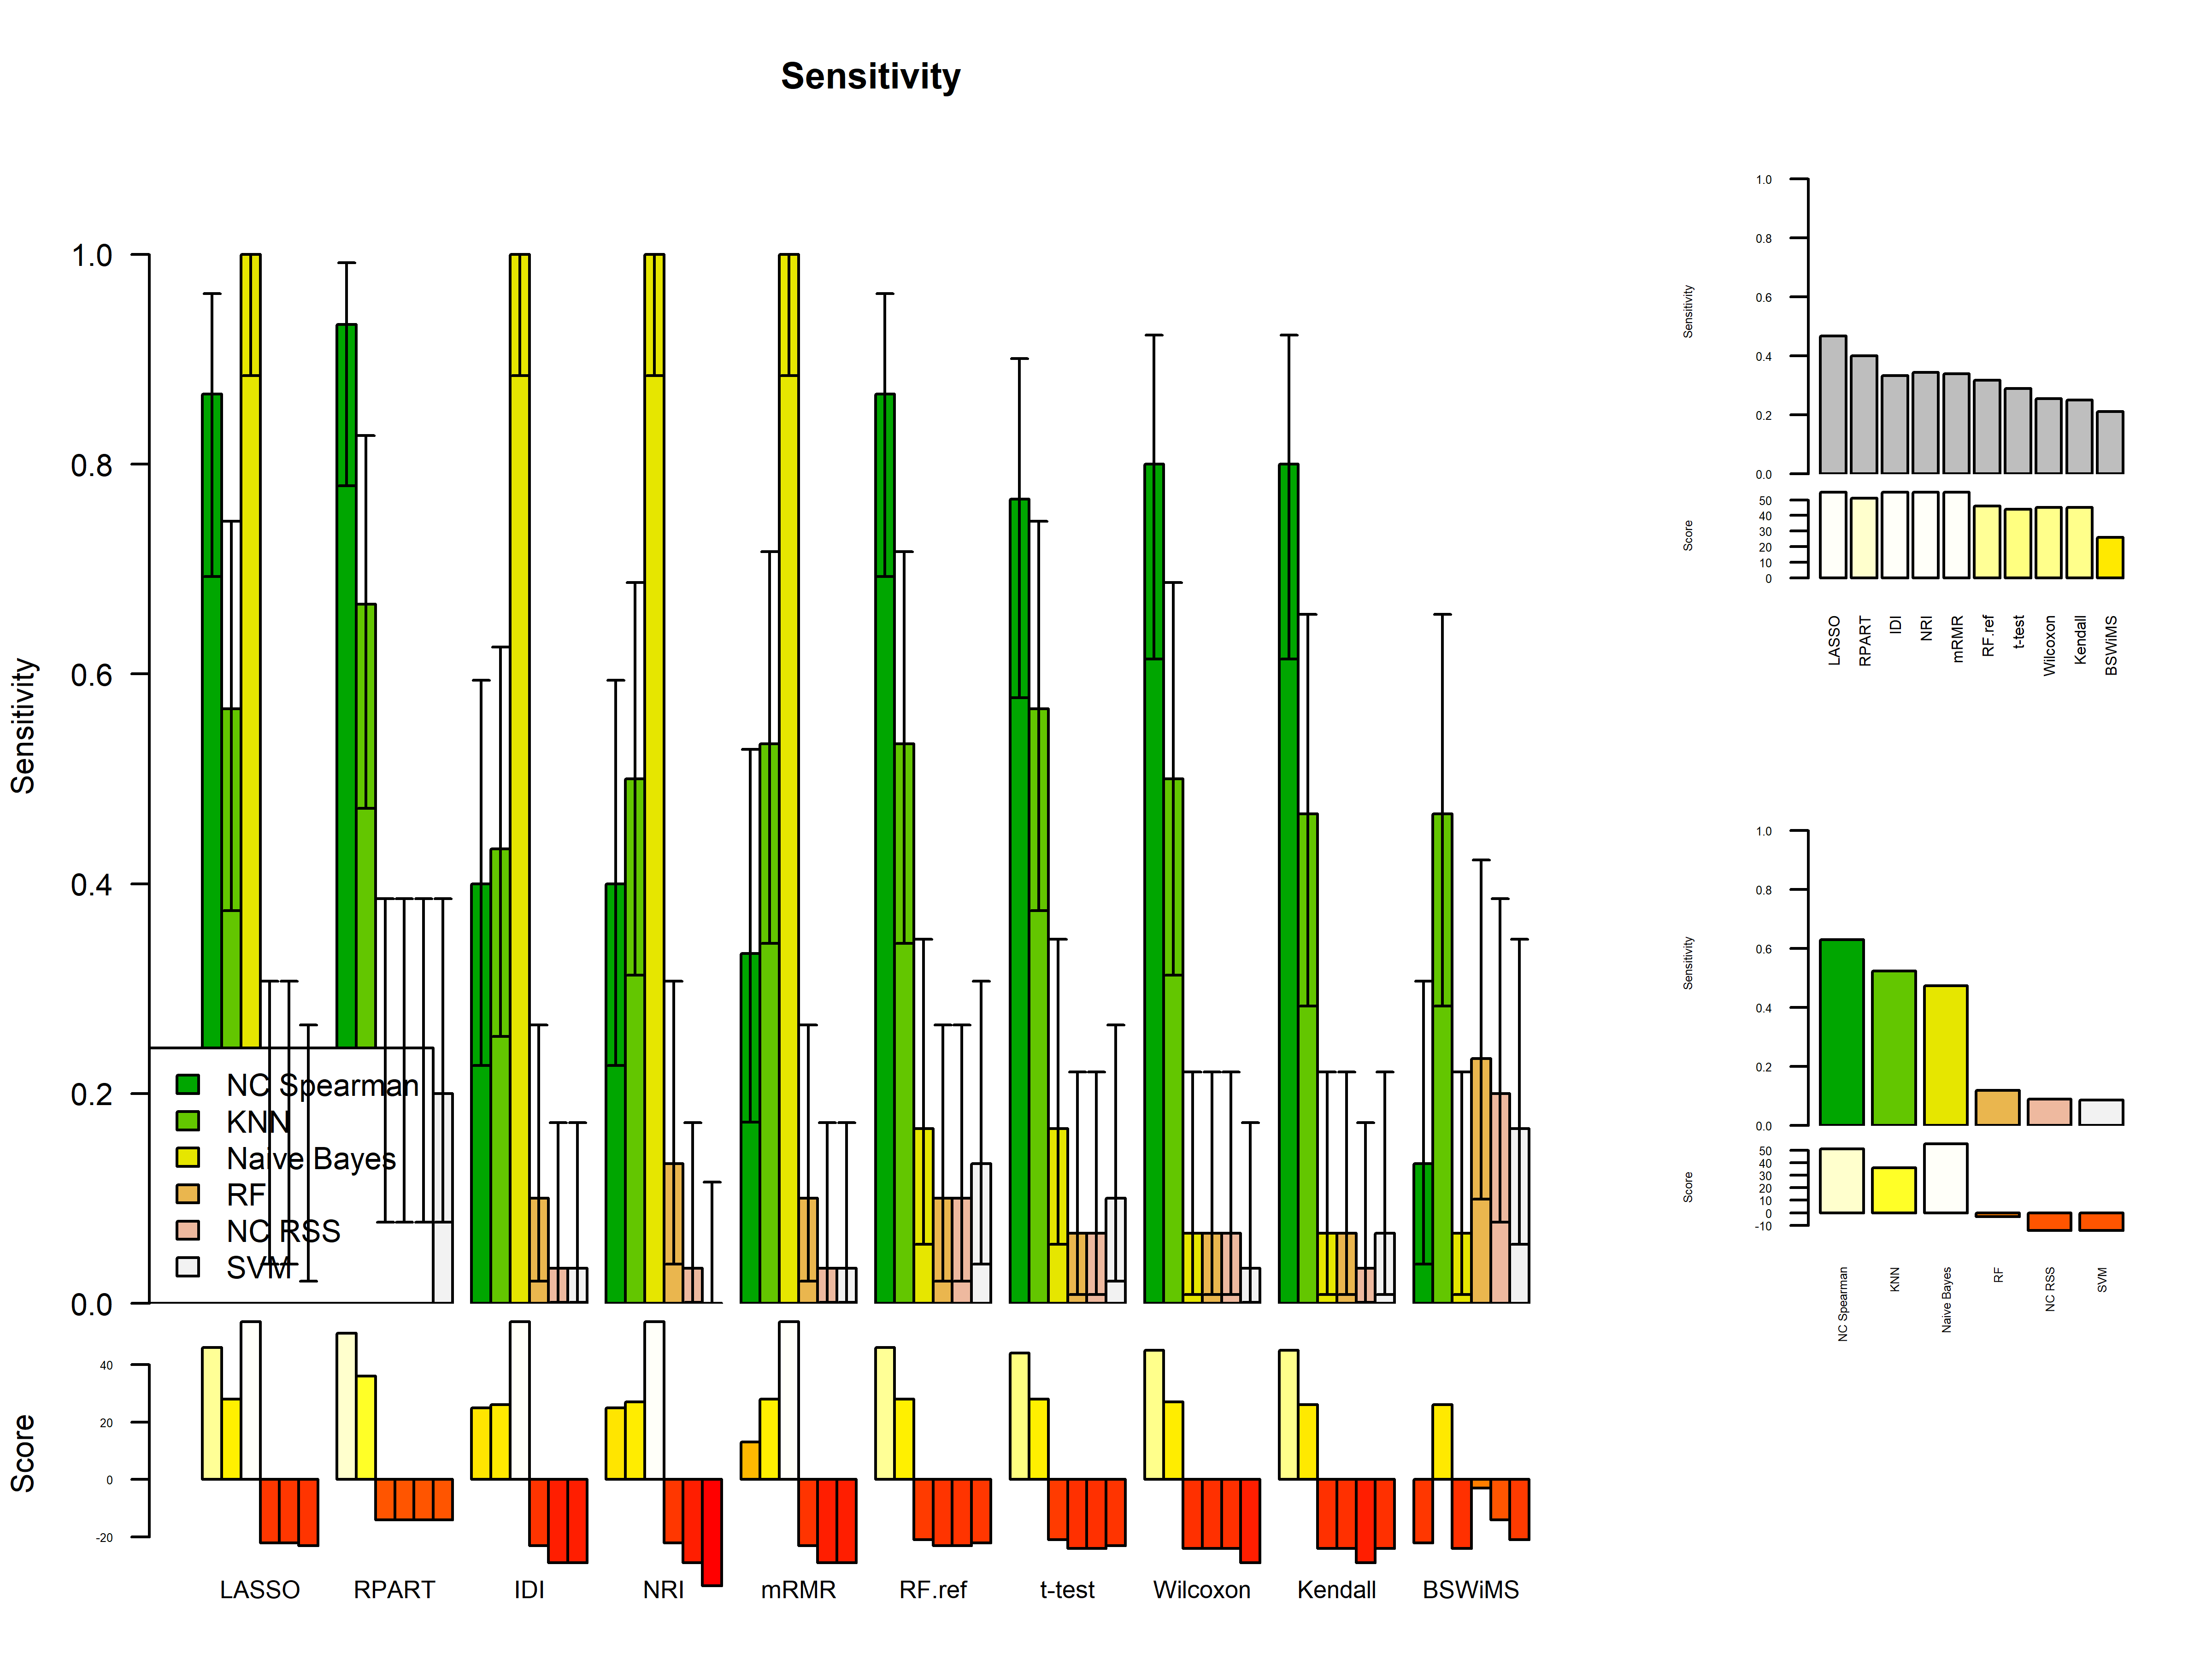
\includegraphics[width=5in,height=2in]{images/results/fresaSensVal.png}}
\centerline{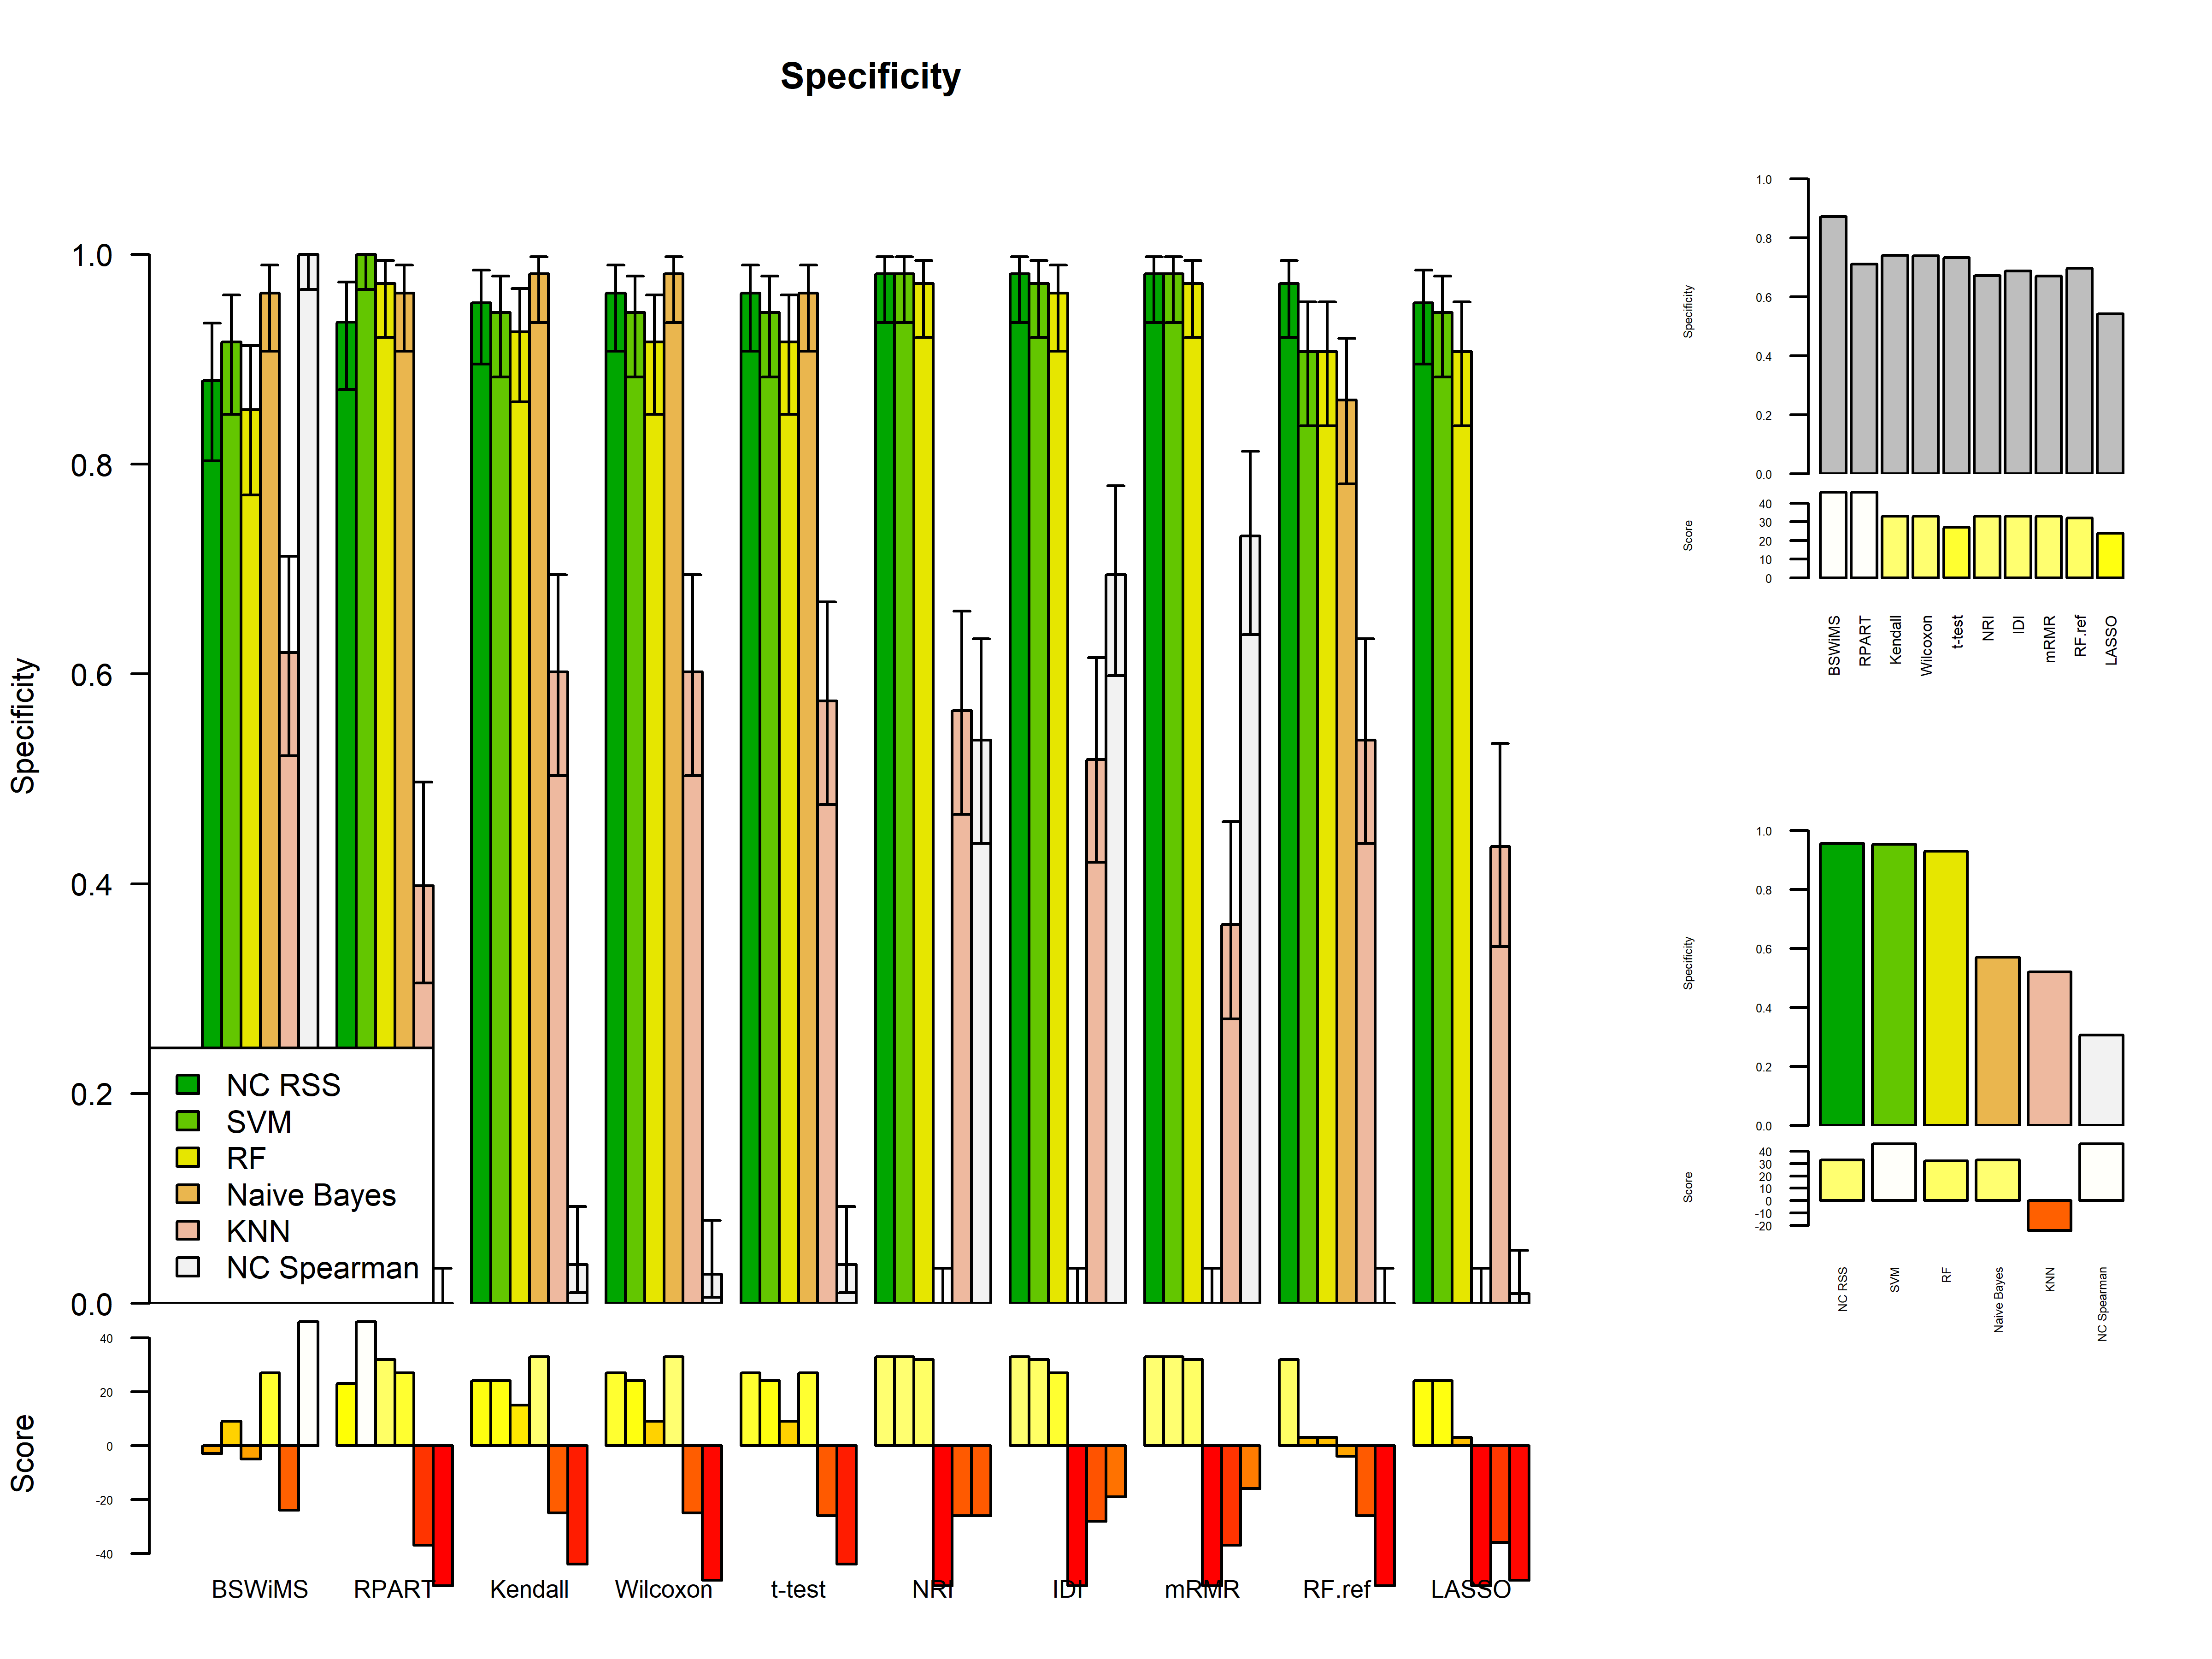
\includegraphics[width=5in,height=2in]{images/results/fresaSpecVal.png}}
\caption{{\bf Validation ROC AUC, Sensitivity and Specificity of the FRESA.CAD Filter combinations} 
Comparison the ROC AUC, Sensitivity and Specificity Score obtained using the different combinations of classification methods plus filters of the FRESA.CAD Benchmarking with the validation dataset for the Cross-validation and using the top 1,000 SNPs as input}
\label{fig22}
\end{figure}
\clearpage
When performing the Meta-Analysis to detect candidate SNPs a much different situation happens than before. As shown in Figure 4.23 there are much more SNPs being selected with a frequency higher than 0.1, which could be interpreted as having less certainty of the SNPs that provide a stronger classification probability. Table 2 seems to back this too, as there are multiple . Coincidentally, the SNPs selected previously are not the same ones as before. APOE $\epsilon4$ is definitely the top marker again, but only rs6448799 appears on both besides APOE $\epsilon4$, thus leading to believe that the SNPs being selected could be either statistical coincidences due to the small amount of samples, or behaving differently now that there is no IGAP information leakage. RPART also appears to not include APOE $\epsilon4$ and still achieve good results, which is certainly odd. As described before, the ROC AUC scores are higher than the actual results obtained in the experiment by far, which reinforces the reason why these scores are not equivalent to the previous ones.
\begin{figure}[!ht]
\centerline{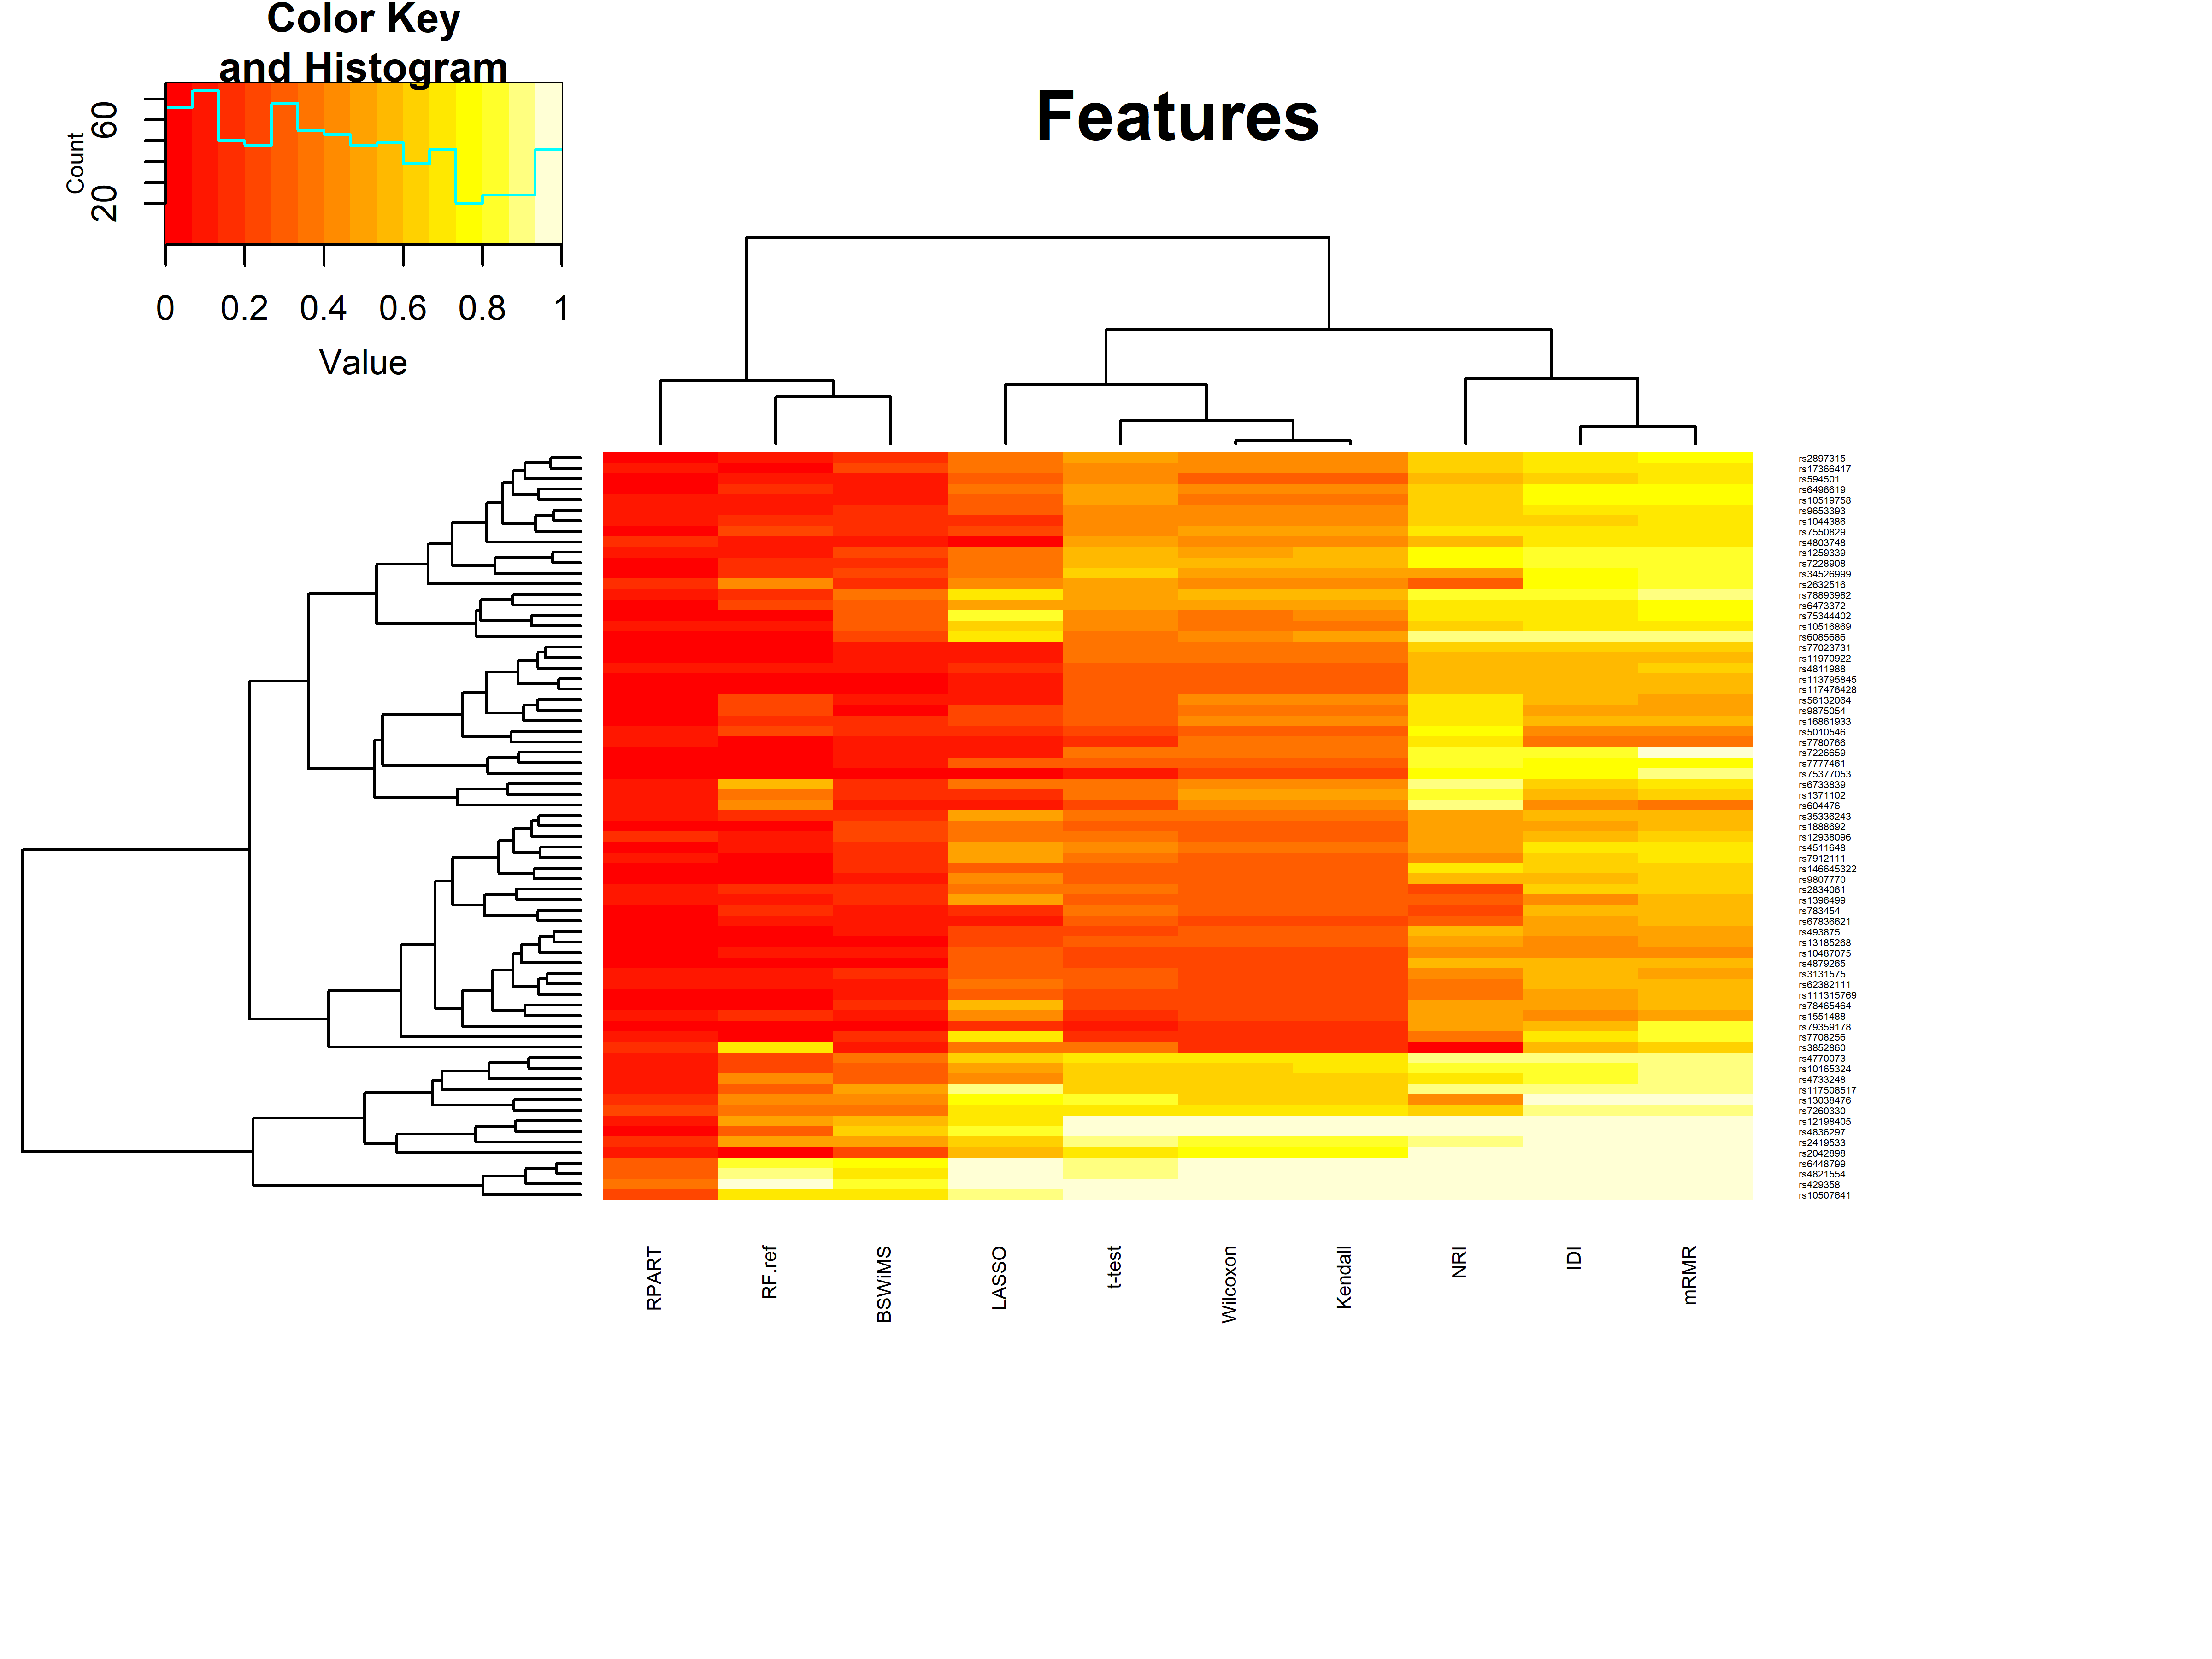
\includegraphics[width=4in]{images/results/fresaSNPsVal.png}}
\caption{{\bf Validation SNPs chosen more than 10\% of the time as features of the FRESA.CAD Benchmark} 
Heatmap of the main SNPs being chosen across all the classifiers. The Y axis are the main SNPs being selected while the X axis represents the different classifiers of the FRESA.CAD Benchmarking with the validation dataset for the Cross-validation and using the top 1,000 SNPs as input}
\label{fig23}
\end{figure}

\begin{table}[ht!]
    \begin{center}
        \begin{tabular}{|c|c|c|c|}
        \hline
        \textbf{SNP}   &  \textbf{ROC AUC} &  \textbf{WILCOX} &  \textbf{FREQ} \\ \hline
rs429358   &	0.684 &	0.0436 &	0.91 \\ \hline
rs6448799  &	0.6614 &	0 &	0.815 \\ \hline
rs4821554	&	0.6537 &	1e-04 &	0.874 \\ \hline
rs7260330	&	0.6383 &	0.0027 &	0.667 \\ \hline
rs10507641	&	0.637 &	0 &	0.797 \\ \hline
rs4733248	&	0.6349 &	0.0052 &	0.581 \\ \hline
rs13038476	&	0.6318 &	0 &	0.627 \\ \hline
rs2419533	&	0.6304 &	0.0013 &	0.716 \\ \hline
rs34526999	&	0.6228 &	0.025 &	0.445 \\ \hline
rs2632516	&	0.6185 &	0.02 &	0.387 \\ \hline
        \end{tabular}
    \end{center}
  \caption{Top  SNPs selected as important features for the Validation dataset}
  \label{topsnps2}
\end{table}

\clearpage
\section{LDPred-funct}

The results of the LDPred-funct are not very interesting. As an intermediate metric the $h^2$ score is calculated, which in rough terms  gives the heritability of the disease, in this case the result is a value of 0.06 based on the IGAP statistics which basically means that the heritability component of the disease statistically found is not very high, this result is consistent with other analysis done previously. As a contrast, the phenotype height is shown to be 0.58 in the LDPred-funct paper.

LDPred-funct then returns an $r^2$ value of 0.025. A more layman representation is to say that the PRS calculated by LDPred-funct can explain 42\% of the expected heritability limit, and that the method can explain 3\% of the variance shown in the disease. This is a low value and is also represented in the Polygenic Risk Score. When using it to classify between cases and controls the PRS assigns every sample in the ADNI validation dataset as a case. This means that the ROC score is 0.50 and for classification purposes is not useful.

Now, this result and low heritability calculation are at odds with the APOE $\epsilon4$ statistics. This result is mainly due to the small size of the validation dataset as well as the complexity of Alzheimer's Disease in terms of genetic heritability. It could be that with a much larger validation dataset or using a larger summary statistic for Alzheimer would give more accurate results. Additionally, as the diagnosis of Alzheimer's is post-mortem the summary statistics could also be skewed. But the values obtained are consistent with the results of other complex diseases such as Type 2 Diabetes, Cron's Disease and Schizophrenia \cite{Consortium2009}, which further reinforces the point that AD is highly complex, polygenic and multifactorial.

\section{Discussion}


Previous research on the early detection of late-onset Alzheimer's disease have relied on a variety of clinical biomarkers for disease prediction \cite{Alexiou2017}. The efficacy of experimental treatments and palliative interventions rely heavily on the early detection of the disease \cite{Dufouil2018}. Unfortunately, clinical biomarkers such as beta amyloid and tau proteins are correlated with disease progression. Therefore, their usefulness for the early detection of the disease remains controversial.

The etiology of LOAD is likely to be motivated by both environmental and genetic components. However, the genetic component seems to a major determinant as the heritability of the disease has been estimated to be $\sim$ 80\% \cite{Raghavan2017}. Therefore, genetic testing hold the potential to provided sufficiently accurate predictions of the disease using genetic data exclusively. Unfortunately, the genetic variants with associations with LOAD discovered by GWAS studies are only capable to explain a fraction of this genetic component (33\%). Therefore, methodologies that account for this missing heritability are required to achieve better predictions \cite{Escott015} \cite{Escott2017}.

In this thesis, it is proposed the use of deep neural networks and machine learning  for predicting late-onset Alzheimer's disease from genetic data. This Thesis' hypothesis postulated that the use of a large number of genetic variants would allow us to improve the classification performance of the proposed model. It is expected of the deep learning model to create hierarchical features with the potential to account for the missing heritability of the disease.

Experimental results indicate that classification performance of $\sim$ 65\% AUC can be achieved with the proposed model. In comparison, the use of the APOE $\epsilon4$ gene with the ADNI dataset gives a predictive score of 0.61\% ~ 0.62\% on the Cross-Validation and 56\% ~64\% on the Split Validation depending on the method. Most importantly, the experiments reported here suggest that an increasing number of genetic variants as predictors hold the potential to contribute to improve the predictive capabilities of the proposed model providing that a sufficiently large number of samples are available. 


The deep learning models in particular suffered from overfitting the training data in the experiments (and obtaining a score of 98\%~100\%). Through the use of dropout, normalization and regularization this was controlled but the main way overfitting can be avoided is through the use of a larger sample size . The deep learning models consist of a large number of possible parameters, and as such with a low number of samples the tendency to overfit is larger. By increasing the size of the dataset the overfitting problem will reduce and the model will have a lower variance. Furthermore, another issue with the current dataset is that the number of predictors\/features outnumber the number of samples. This creates a problem where each individual feature could present low variance within the samples to be of statistical use. 

In the majority of experiments reported here, random forest produced better results that deep learning models possibly because of these issues. However, according to empirical observations on the performance of deep learning models in these experiments (especially the simulations) , it is expected the latter to outperform the former as more data becomes available. In general, deep learning models have shown to scale the performance better than other machine learning models with increasing amounts of data \cite{Goodfellow2016}.

\newpage
Simulated models of purely genetic diseases tend to show the models perform as expected, by analyzing a greater number of markers as well as a greater number of samples they are able to obtain better performance. The models were never able to learn with perfect accuracy the underlying causes for the simulated disease, which is to be expected considering that the disease is spread out through 12,000 genes. This could also show what is happening with other diseases, where the factors could be even greater. This does show the value of Machine Learning for Genomic analysis and specifically the importance of using big datasets that can give the full spectrum of information usable to predict precisely.

Data-augmentation in turn did not give results informative enough to validate its use on the first case with using the full dataset, although for the case where only the independent validation set was used by doing Data Augmentation the models were able to perform better than the models where there existed no data augmentation. This could be either because the number of validation data versus the training data is too low and by doing the Data-Augmentation the data set increases sufficiently to increase the performance, or because the validation samples are sufficiently different in terms of gene distribution that the learned features are not useful in the testing set. The second idea is supported by the results obtained in the meta-analysis using FRESA.CAD. 

For the case of the models tested with the FRESA.CAD Benchmark the Ensemble method is able to explain 70\% of the expected genetic component for the given full ADNI Cohort. It can also be seen that the different methods selected as features SNPs which have been reported in the literature to have a correlation with Alzheimer, thus showing that the algorithm is consistent with the results previously found and has a medical basis. The reduced cohort for the independent validation score would then just explain 33\% of the genetic variation, but this could be due to the balance problem as well as the low data set size. The FRESA.CAD Benchmark seems to be a promising tool for Genomics analysis and finding candidate markers.
 
 LDPred-funct was found to have results that were lacking in predictive power but which are slightly consistent with other reported complex diseases. This validates yet again with another approach the difficulty being faced with predicting Alzheimer's Disease. The results on small datasets appear to show that for small samples or test sets the Machine Learning models are better in the prediction task than more statistical approaches to the disease. Given much larger datasets one could expect the LDPred-funct algorithm to perform better than most machine learning algorithms.
 \newpage
 LOAD prediction is a challenging problem. In effect, the etiology and the genetic architecture of the disease remain unexplained. Moreover, accurate diagnosis of the disease is still an open problem. Therefore, labeled datasets including confirmatory diagnosis are not currently available. This data would be critical for the construction of accurate predictive models. Further research and development of models could open avenues to increase the certainty of the diagnosis that could in the long run increase the precision of predictive models.

In addition, it is unclear whether or not there are useful genetic variants that account for the transition from mild cognitive impairment to LOAD. According to recent studies, currently available LOAD polygenic scores are not capable to predict mild cognitive impairment to LOAD progression \cite{Lacour2016}. Therefore, alternative models are also required for the accurate prediction of disease progression.